% Options for packages loaded elsewhere
\PassOptionsToPackage{unicode}{hyperref}
\PassOptionsToPackage{hyphens}{url}
\PassOptionsToPackage{dvipsnames,svgnames*,x11names*}{xcolor}
%
\documentclass[
  lualatex,ja=standard,jafont=noto-otf]{bxjsreport}
\usepackage{lmodern}
\usepackage{amssymb,amsmath}
\usepackage{ifxetex,ifluatex,ifpdf,ifthen}
\ifnum 0\ifxetex 1\fi\ifluatex 1\fi=0 % if pdftex
  \usepackage[T1]{fontenc}
  \usepackage[utf8]{inputenc}
  \usepackage{textcomp} % provide euro and other symbols
\else % if luatex or xetex
  \usepackage{unicode-math}
  \defaultfontfeatures{Scale=MatchLowercase}
  \defaultfontfeatures[\rmfamily]{Ligatures=TeX,Scale=1}
  \setmonofont[]{Ricty Discord}
\fi

% japanese font setting
% if the preset is specified
\ifxetex
  \usepackage{xeCJKfntef}
\fi
\ifluatex
  \usepackage{luatexja}
  \usepackage[,noto-otf]{luatexja-preset}
\fi

  \IfFileExists{pxrubrica.sty}{\usepackage{pxrubrica}}{}
\ifluatex
  \ltjsetparameter{%
    jacharrange={-2,-3},
    alxspmode={`/,allow},
    alxspmode={`#,allow},
    alxspmode={92,allow}
  }
\fi


% Use upquote if available, for straight quotes in verbatim environments
\IfFileExists{upquote.sty}{\usepackage{upquote}}{}
\ifpdf
  \IfFileExists{microtype.sty}{% use microtype if available
    \usepackage[]{microtype}
    \UseMicrotypeSet[protrusion]{basicmath} % disable protrusion for tt fonts
  }{}
\fi
\makeatletter
\@ifundefined{KOMAClassName}{% if non-KOMA class
  \IfFileExists{parskip.sty}{%
    \usepackage{parskip}
  }{% else
    \setlength{\parindent}{0pt}
    \setlength{\parskip}{6pt plus 2pt minus 1pt}}
}{% if KOMA class
  \KOMAoptions{parskip=half}}
\makeatother
\usepackage{xcolor}
\IfFileExists{xurl.sty}{\usepackage{xurl}}{} % add URL line breaks if available
\IfFileExists{bookmark.sty}{\usepackage{bookmark}}{\usepackage{hyperref}}
\hypersetup{
  pdftitle={knitr: Rによる美麗で柔軟そして高速な動的レポート生成},
  pdfauthor={著者: Xie, Yihui (谢益辉); 翻訳者: Katagiri, Satoshi (片桐 智志)},
  colorlinks=true,
  linkcolor=blue,
  filecolor=Maroon,
  citecolor=blue,
  urlcolor=magenta,
  pdfcreator={LaTeX via pandoc}}
\urlstyle{same} % disable monospaced font for URLs
\usepackage{color}
\usepackage{fancyvrb}
\newcommand{\VerbBar}{|}
\newcommand{\VERB}{\Verb[commandchars=\\\{\}]}
\DefineVerbatimEnvironment{Highlighting}{Verbatim}{commandchars=\\\{\}}
% Add ',fontsize=\small' for more characters per line
\usepackage{framed}
\definecolor{shadecolor}{RGB}{248,248,248}
\newenvironment{Shaded}{\begin{snugshade}}{\end{snugshade}}
\newcommand{\AlertTok}[1]{\textcolor[rgb]{0.94,0.16,0.16}{#1}}
\newcommand{\AnnotationTok}[1]{\textcolor[rgb]{0.56,0.35,0.01}{\textbf{\textit{#1}}}}
\newcommand{\AttributeTok}[1]{\textcolor[rgb]{0.77,0.63,0.00}{#1}}
\newcommand{\BaseNTok}[1]{\textcolor[rgb]{0.00,0.00,0.81}{#1}}
\newcommand{\BuiltInTok}[1]{#1}
\newcommand{\CharTok}[1]{\textcolor[rgb]{0.31,0.60,0.02}{#1}}
\newcommand{\CommentTok}[1]{\textcolor[rgb]{0.56,0.35,0.01}{\textit{#1}}}
\newcommand{\CommentVarTok}[1]{\textcolor[rgb]{0.56,0.35,0.01}{\textbf{\textit{#1}}}}
\newcommand{\ConstantTok}[1]{\textcolor[rgb]{0.00,0.00,0.00}{#1}}
\newcommand{\ControlFlowTok}[1]{\textcolor[rgb]{0.13,0.29,0.53}{\textbf{#1}}}
\newcommand{\DataTypeTok}[1]{\textcolor[rgb]{0.13,0.29,0.53}{#1}}
\newcommand{\DecValTok}[1]{\textcolor[rgb]{0.00,0.00,0.81}{#1}}
\newcommand{\DocumentationTok}[1]{\textcolor[rgb]{0.56,0.35,0.01}{\textbf{\textit{#1}}}}
\newcommand{\ErrorTok}[1]{\textcolor[rgb]{0.64,0.00,0.00}{\textbf{#1}}}
\newcommand{\ExtensionTok}[1]{#1}
\newcommand{\FloatTok}[1]{\textcolor[rgb]{0.00,0.00,0.81}{#1}}
\newcommand{\FunctionTok}[1]{\textcolor[rgb]{0.00,0.00,0.00}{#1}}
\newcommand{\ImportTok}[1]{#1}
\newcommand{\InformationTok}[1]{\textcolor[rgb]{0.56,0.35,0.01}{\textbf{\textit{#1}}}}
\newcommand{\KeywordTok}[1]{\textcolor[rgb]{0.13,0.29,0.53}{\textbf{#1}}}
\newcommand{\NormalTok}[1]{#1}
\newcommand{\OperatorTok}[1]{\textcolor[rgb]{0.81,0.36,0.00}{\textbf{#1}}}
\newcommand{\OtherTok}[1]{\textcolor[rgb]{0.56,0.35,0.01}{#1}}
\newcommand{\PreprocessorTok}[1]{\textcolor[rgb]{0.56,0.35,0.01}{\textit{#1}}}
\newcommand{\RegionMarkerTok}[1]{#1}
\newcommand{\SpecialCharTok}[1]{\textcolor[rgb]{0.00,0.00,0.00}{#1}}
\newcommand{\SpecialStringTok}[1]{\textcolor[rgb]{0.31,0.60,0.02}{#1}}
\newcommand{\StringTok}[1]{\textcolor[rgb]{0.31,0.60,0.02}{#1}}
\newcommand{\VariableTok}[1]{\textcolor[rgb]{0.00,0.00,0.00}{#1}}
\newcommand{\VerbatimStringTok}[1]{\textcolor[rgb]{0.31,0.60,0.02}{#1}}
\newcommand{\WarningTok}[1]{\textcolor[rgb]{0.56,0.35,0.01}{\textbf{\textit{#1}}}}
% for compatible with kableExtra package functions.
\usepackage{longtable,booktabs,dcolumn}
%\usepackage{longtable,booktabs,dcolumn,array,multirow,wrapfig,float,colortbl,pdflscape,tabu,threeparttable,threeparttablex,makecell}
% Correct order of tables after \paragraph or \subparagraph
\usepackage{etoolbox}
\makeatletter
\patchcmd\longtable{\par}{\if@noskipsec\mbox{}\fi\par}{}{}
\makeatother
% Allow footnotes in longtable head/foot
\IfFileExists{footnotehyper.sty}{\usepackage{footnotehyper}}{\usepackage{footnote}}
\makesavenoteenv{longtable}
\usepackage{graphicx,grffile}
\makeatletter
\def\maxwidth{\ifdim\Gin@nat@width>\linewidth\linewidth\else\Gin@nat@width\fi}
\def\maxheight{\ifdim\Gin@nat@height>\textheight\textheight\else\Gin@nat@height\fi}
\makeatother
% Scale images if necessary, so that they will not overflow the page
% margins by default, and it is still possible to overwrite the defaults
% using explicit options in \includegraphics[width, height, ...]{}
\setkeys{Gin}{width=\maxwidth,height=\maxheight,keepaspectratio}
% Set default figure placement to htbp
\makeatletter
\def\fps@figure{htbp}
\makeatother
\setlength{\emergencystretch}{3em} % prevent overfull lines
\providecommand{\tightlist}{%
  \setlength{\itemsep}{0pt}\setlength{\parskip}{0pt}}
\setcounter{secnumdepth}{5}


% compatible mukti-columns macro
% by "R Markdown Cookbook" Sec. 5.8
\newenvironment{cols}[1][]{}{}
\newenvironment{col}[1]{\begin{minipage}{#1}\ignorespaces}{%
\end{minipage}
\ifhmode\unskip\fi
\aftergroup\useignorespacesandallpars}
\def\useignorespacesandallpars#1\ignorespaces\fi{%
#1\fi\ignorespacesandallpars}
\makeatletter
\def\ignorespacesandallpars{%
\@ifnextchar\par
{\expandafter\ignorespacesandallpars\@gobble}%
{}%
}
\makeatother
%-------


% ---- XeLaTeX 専用のあれ ----
\ifxetex
  \usepackage{letltxmacro}
  \setlength{\XeTeXLinkMargin}{1pt}
  \LetLtxMacro\SavedIncludeGraphics\includegraphics
  \def\includegraphics#1#{% #1 catches optional stuff (star/opt. arg.)
    \IncludeGraphicsAux{#1}%
  }%
  \newcommand*{\IncludeGraphicsAux}[2]{%
    \XeTeXLinkBox{%
      \SavedIncludeGraphics#1{#2}%
    }%
  }%
\fi

% ---- custom blocks ----
\makeatletter
\newenvironment{kframe}{%
\medskip{}
\setlength{\fboxsep}{.8em}
 \def\at@end@of@kframe{}%
 \ifinner\ifhmode%
  \def\at@end@of@kframe{\end{minipage}}%
  \begin{minipage}{\columnwidth}%
 \fi\fi%
 \def\FrameCommand##1{\hskip\@totalleftmargin \hskip-\fboxsep
 \colorbox{shadecolor}{##1}\hskip-\fboxsep
     % There is no \\@totalrightmargin, so:
     \hskip-\linewidth \hskip-\@totalleftmargin \hskip\columnwidth}%
 \MakeFramed {\advance\hsize-\width
   \@totalleftmargin\z@ \linewidth\hsize
   \@setminipage}}%
 {\par\unskip\endMakeFramed%
 \at@end@of@kframe}
\makeatother

\makeatletter
\@ifundefined{Shaded}{
}{\renewenvironment{Shaded}{\begin{kframe}}{\end{kframe}}}
\makeatother


% --- custom blocks ---

% ---- redefine quote format as modern
\setlength{\fboxsep}{.8em}
\usepackage{framed}
\definecolor{quotebarcolor}{rgb}{0.2,0.2,0.2}
\renewenvironment{quote}{\def\FrameCommand{{\color{quotebarcolor}{\vrule width 3pt}}\hspace{10pt}}\MakeFramed{\advance\hsize-\width\FrameRestore}}{\endMakeFramed}
% ----
% ---- tcolobox settings by the Cookbook Sec.9.6.2
\usepackage{tcolorbox}
% \newenvironment{blackbox}{\definecolor{shadecolor}{rgb}{0, 0, 0}\color{white}\begin{shaded}}{\end{shaded}}
% \newtcolorbox{blackbox}{colback=black,colframe=orange,coltext=white,boxsep=5pt,arc=4pt}
\newtcolorbox{greyblock}{colback=gray!20,colframe=orange,coltext=black,boxsep=5pt,arc=4pt}
\newenvironment{infobox}[1]{\begin{itemize}\renewcommand{\labelitemi}{\raisebox{-.7\height}[0pt][0pt]{%
  {\setkeys{Gin}{width=3em,keepaspectratio}\includegraphics{_latex/_img/#1}}}}
  \setlength{\fboxsep}{1em}
  \begin{greyblock}
  \item
  }{\end{greyblock}\end{itemize}
}
% ----

% for block/block2 engine
\newenvironment{memo}{\begin{infobox}{memo}}{\end{infobox}}
\newenvironment{caution}{\begin{infobox}{caution}}{\end{infobox}}
\newenvironment{important}{\begin{infobox}{important}}{\end{infobox}}
\newenvironment{tip}{\begin{infobox}{tip}}{\end{infobox}}
\newenvironment{warning}{\begin{infobox}{warning}}{\end{infobox}}
% ---- custom block over ----

% --- for soft wrapping in code block
\usepackage{fvextra}
\DefineVerbatimEnvironment{Highlighting}{Verbatim}{commandchars=\\\{\},breaklines,breakanywhere}
% ----

% ---- font style-changing macro for convenient ----
\ifdefined\mcfamily
  \newcommand{\textserif}[1]{{\rmfamily\mcfamily #1}}
\else
  \newcommand{\textserif}[1]{{\rmfamily #1}}
\fi
\ifdefined\gtfamily
  \newcommand{\textsans}[1]{{\sffamily\gtfamily #1}}
\else
  \newcommand{\textsans}[1]{{\sffamily #1}}
\fi
% ----

% ---- user-defined preamble here ----
% ---- user-defined preamble over ----

\usepackage[style=jauthoryear,natbib=true]{biblatex}


\title{\textbf{knitr}: Rによる美麗で柔軟そして高速な動的レポート生成}
\author{著者: Xie, Yihui (谢益辉) \and 翻訳者: Katagiri,
Satoshi\footnote{twitter@\href{https://twitter.com/ill_identified}{ill\_identified}}
(片桐 智志)}
\date{ver. 1.6 (2022/02/19 00:40:13 JST, 本家最終更新時刻:
\href{https://github.com/rbind/yihui/tree/master/content/knitr}{2022/01/25
16:17:20 JST})}
\usepackage{bxtexlogo}
\colorlet{shadecolor}{gray!20}

\usepackage{fmtcount}
\ifdefined\theFancyVerbLine\renewcommand{\theFancyVerbLine}{\small \padzeroes[2]{\decimal{FancyVerbLine}}}\fi % adjust row number position
\IfFileExists{bxcoloremoji.sty}{\usepackage{bxcoloremoji}}{}




\begin{document}
\maketitle

{
\hypersetup{linkcolor=}
\setcounter{tocdepth}{2}
\tableofcontents
}
\hypertarget{knitr}{%
\chapter*{knitr}\label{knitr}}
\addcontentsline{toc}{chapter}{knitr}

\begin{infobox}{important}
本稿は
\href{https://creativecommons.org/licenses/by-nc-sa/4.0/deed.ja}{CC
BY-NC-SA 4.0 (クリエイティブ・コモンズ 表示 - 非営利 - 継承 4.0
国際)ライセンス} で提供されています. Yihui 氏によるオリジナルは
\url{https://yihui.org/knitr/} で読むことができます.

This is an unofficial Japanese translation of Yihui's \textbf{knitr}
documentation, which is licensed under
\href{https://creativecommons.org/licenses/by-nc-sa/4.0/}{CC BY-NC-SA
4.0}. The original documentation by Yihui is
\href{https://yihui.org/knitr/}{here}.

\end{infobox}

\href{https://creativecommons.org/licenses/by-nc-sa/4.0/deed.ja}{\includegraphics{./7051e470f21a5ffaacd91435e622cbb2e1382765.png}}

\begin{infobox}{tip}
\textbf{訳注}: Yihui
氏のサイトの一連のドキュメントはかなり以前から氏のブログ投稿として断続的に更新されてきたものを編纂しているため,
内容の重複した記述がいくつかありますし, RStudio および R Markdown
が普及している現在では, やや out-of-date な記述も見られます (現在では
Sweave はあまり使いません). そのため,
\textbf{サイドバーの目次から辿れるページ,
およびそれらでリンクされているページ以外は重要度が低いと見なし,
翻訳していません}. 同様の理由から「用例」も一部を除き翻訳していません
(\textbf{共同翻訳者は常に歓迎します}:
\url{https://github.com/Gedevan-Aleksizde/knitr-doc-ja}).

しかしながら翻訳時の \textbf{knitr} および R Markdown
に関する日本語の情報流通を鑑みるに,
非常に有用なドキュメントであると翻訳者は確信しています.
それぞれのトピックがどの環境を想定したものなのか,
よく確認してご覧ください.

\end{infobox}

\hypertarget{ux6982ux8981}{%
\section*{概要}\label{ux6982ux8981}}
\addcontentsline{toc}{section}{概要}

\textbf{knitr} パッケージは R
を使用した透明な動的なレポート作成エンジンとしてデザインされ,
長年にわたって存在した Sweave
の問題を解決するとともに他のアドオンパッケージの機能を統合しています
(\textbf{knitr} ≈ Sweave + cacheSweave + pgfSweave + weaver +
\texttt{animation::saveLatex} + \texttt{R2HTML::RweaveHTML} +
\texttt{highlight::HighlightWeaveLatex} + 0.2 * brew + 0.1 *
SweaveListingUtils + その他).

\href{https://amzn.com/1498716962}{}

\begin{itemize}
\tightlist
\item
  透明性とはユーザーが入力と出力に完全にアクセスできることを意味します.
  例えば R ターミナル上では \texttt{1\ +\ 2} は \texttt{{[}1{]}\ 3}
  を出力しますが, \textbf{knitr}によってユーザーは \texttt{1\ +\ 2} を
  LaTeX の \texttt{\textbackslash{}begin\{verbatim\}} と
  \texttt{\textbackslash{}end\{verbatim\}} や, HTML タグ
  \texttt{\textless{}div\ class="rsource"\textgreater{}} と
  \texttt{\textless{}/div\textgreater{}} の間に出力したりできますし,
  \texttt{{[}1{]}\ 3} を \texttt{\textbackslash{}begin\{Routput\}} と
  \texttt{\textbackslash{}end\{Routput\}} の間に出力できたりします.
  詳細は \ref{hooks} 章『フック』を参照してください.
\item
  \textbf{knitr} は R コードを
  Rターミナル上で実行した場合でもユーザーの意図する結果と一致することを目指しています.
  例えば \texttt{qplot(x,\ y)} でそのままグラフを出力できます
  (\texttt{print()} は不要です) し,
  デフォルトでコードチャンク内の\textbf{全ての}プロットが出力されます.
\item
  \textbf{\texttt{pgfSweave}} や \textbf{\texttt{cacheSweave}}
  といったパッケージは有用な機能を Sweave に提供しました (高品質な tikz
  のグラフィックとキャッシュ) が, \textbf{knitr}
  はこの実装をより簡単にしました.
\item
  \textbf{knitr} のデザインによってあらゆる言語 (例: R, Python, awk)
  が入力可能となり,
  あらゆるマークアップ言語の形式で出力が可能となりました (例: LaTeX,
  HTML, Markdown, AsciiDoc, reStructuredText).
\end{itemize}

このパッケージは \href{https://github.com/yihui/knitr}{GitHub}
上で開発されており,
インストール手順と\protect\hyperlink{FAQs}{FAQ}もここで参照できます.
\href{https://github.com/yihui/knitr\#readme}{パッケージの README}
も確認してください. このサイトは \textbf{knitr}
の完全なドキュメントとして提供されており,
\protect\hyperlink{manual}{メインマニュアル},
\protect\hyperlink{graphics}{グラフィックス},
\protect\hyperlink{examples}{用例},
\href{https://github.com/yihui/knitr-examples}{knitr-examples}
を閲覧することができます. さらに統合的な参考資料としては,
\href{https://github.com/yihui/knitr-book}{knitr book} (邦訳未刊行)
をご覧ください.

\hypertarget{ux30e2ux30c1ux30d9ux30fcux30b7ux30e7ux30f3}{%
\section*{モチベーション}\label{ux30e2ux30c1ux30d9ux30fcux30b7ux30e7ux30f3}}
\addcontentsline{toc}{section}{モチベーション}

Sweave の拡張の難しいところは \textbf{\texttt{utils}}
パッケージから大量のコードをコピーする必要があることでした
(\texttt{SweaveDrivers.R} のコードは700行を超えています).
そしてこれは上述の2つのパッケージ両方での作業です.
コードをコピーペーストしたら, パッケージ開発者は R
の公式バージョンの変更にとても慎重に対応せねばなりません ---
うんざりする仕事だとは思いませんか. \textbf{knitr} パッケージでは sweave
の処理の全行程を小規模な管理しやすい関数群へとモジュール化したため,
喜ばしいことにメンテナンスも機能拡張も容易になりました (例えば簡単に
HTML への対応もできるようになりました). その一方で \textbf{knitr}
は多くのビルトイン機能を持ちますが,
パッケージの機能のコア部分をハックする必要のないようになっています.
そして, Sweave のマニュアルの FAQ の項目にあったいくつかの問題は,
\textbf{knitr} は直接解決することができます.

\begin{quote}
旧態依然とした態度をプログラム構造へと変えましょう.
「我々の主な仕事は何をすべきかコンピュータに教えることである」と考えるのをやめ,
むしろ「人間に対してコンピュータにさせたかったことを説明する」ように注力することです

--- ドナルド E. クヌース 『文芸的プログラミング』, 1984
\end{quote}

\hypertarget{ux7279ux5fb4}{%
\section*{特徴}\label{ux7279ux5fb4}}
\addcontentsline{toc}{section}{特徴}

本パッケージのアイディアは他のパッケージから借用し, いくつか
(キャッシュなど) は異なる形で再実装されています.
以下にパッケージの特徴をいくつか挙げます:

\begin{itemize}
\tightlist
\item
  \textbf{信頼性の高い}出力: バックエンドで
  \href{https://cran.rstudio.com/package=evaluate}{\textbf{\texttt{evaluate}}}
  を使用することで, \textbf{knitr} においてあらゆるコードは,
  結果のプリント, グラフのプロットそして警告・メッセージ・エラーでさえ,
  R ターミナルでするのと同様に書き出されます.
  (厳密にプログラミングする場合, これらは無視するべきではありません.
  特に警告は).

  \begin{itemize}
  \tightlist
  \item
    \textbf{\texttt{ggplot2}} や \textbf{\texttt{lattice}}
    のようなグリッドベースのグラフィックパッケージでは,
    ユーザーはしばしば \texttt{print()} を書くのを忘れてしまう,
    これは些細な問題です. 実際に R ターミナルで出力する時に
    \texttt{print()} は不要ですから. \textbf{knitr}
    ではあなたが意図したとおりの結果を得ることができます.
  \end{itemize}
\item
  キャッシュ機能の組み込み: \textbf{\texttt{cacheSweave}} のようですが,
  しかし \textbf{knitr} ではキャッシュの保存や遅延読み込みのため base R
  の関数を直接使い,
  そして最も顕著な違いはキャッシュされたチャンクは依然として出力もできることです
  (\textbf{\texttt{cacheSweave}} ではキャッシュされたチャンクは.
  \texttt{print()} を明示的に書いたとしても何も出力しませんが,
  \textbf{knitr} はキャッシュされても通常通り出力します).
\item
  R コードの整形: R コードの自動整形に
  \href{https://yihui.org/formatr/}{\textbf{formatR}}
  パッケージが使用されます (長い行の折り返し,
  スペースとインデントの追加, など). これは \texttt{keep.source=FALSE}
  としてもコメントが犠牲になることはありません.
\item
  20 を超えるグラフィックデバイスを直接サポートしています.
  チャンクオプションに
  \texttt{dev=\textquotesingle{}CairoPNG\textquotesingle{}} と書けば,
  すぐさま \href{https://cran.rstudio.com/package=Cairo}{\textbf{Cairo}}
  パッケージの \texttt{CairoPNG()} に切り替えることができますし,
  \texttt{dev=\textquotesingle{}tikz\textquotesingle{}} なら
  \href{https://cran.rstudio.com/package=tikzDevice}{\textbf{tikzDevice}}
  パッケージの \texttt{tikz()} に切り替えられます.
  これ以上簡単にすることなどできないでしょう? これらの組み込みのデバイス
  (正確に言うならラッパー) は単位にインチを使用しています.
  ビットマップでもです (ピクセルは \texttt{dpi}
  オプションに基づいて変換されます. デフォルトは 72 です).
\item
  グラフィックスにおけるさらなる柔軟性:

  \begin{itemize}
  \tightlist
  \item
    出力の幅と高さをさらに指定することが出来ます (\texttt{fig.width}
    はグラフィックデバイスのオプションで, \texttt{out.width}
    は文書に出力する際のものです. たとえば LaTeX なら
    \texttt{out.width=\textquotesingle{}.8\textbackslash{}\textbackslash{}textwidth\textquotesingle{}}
    とします.)
  \item
    グラフの位置も再調整できます.
    グラフが生成された位置に正確に掲載することも,
    チャンクとまとめて表示することもできます
    (\texttt{fig.show=\textquotesingle{}hold\textquotesingle{}}
    オプションを使用してください).
  \item
    最後のグラフだけ欲しいというのでない限り
    (\texttt{fig.keep=\textquotesingle{}last\textquotesingle{}}
    オプションを使用してください),
    コードチャンクごとに複数のグラフが保存されます.
  \end{itemize}
\item
  R コードはコードチャンクに直接書くだけでなく, 他の R
  スクリプトファイルから読み込むこともでき,
  文書を書きながらコードを実行するのが簡単になりました (特に LyX
  で有益です).
\item
  パワーユーザーのために, さらなるカスタマイズが可能になっています.

  \begin{itemize}
  \tightlist
  \item
    Rコードをパースする際に正規表現は拒否されます. つまり,
    \texttt{\textless{}\textless{}\textgreater{}\textgreater{}=},
    \texttt{@}, \texttt{\textbackslash{}Sexpr\{\}}
    などを使う必要はありません.
    もしやりたいのなら任意のパターンを使用できます. 例:
    \texttt{\%\%\ begin.rcode}, \texttt{\%\%\ end.rcode}.
  \item
    フック (hook) は出力の制御を拒否します.
    例えばエラーメッセージを赤い太字で表示したいとしたら,
    ソースコードをイタリック体で表示したいとしたら,
    フック機能をコードの実行前および実行語に定義することが出来ます.
    フック機能はこのパッケージの力を無限に拡大する可能性を持ちます.
    (例えば, アニメーションとか, rgl 3D プロットとか\ldots)
  \end{itemize}
\end{itemize}

多くの取り組みが,
デフォルトでの美しい出力と可読性の向上をもたらしています.
例えばコードチャンクはシンタックスハイライトされて表示され, LaTeX
ではさらに (\href{https://www.ctan.org/pkg/framed}{\textbf{framed}}
パッケージを使うことで) 薄灰色の背景色がつきます.
そのため他のテキストよりやや目立って表示されます. 読書体験はきっと
\texttt{verbatim} や \texttt{Verbatim}
環境を使うよりも良いものとなります. プロンプトで表示される先頭の
\texttt{\textgreater{}} や \texttt{+}
はデフォルトでは\textbf{出力されません} (\texttt{prompt=TRUE}
で表示することもできます). このような記号はコードに割り込んでくるので,
コードをコピーして自分で実行する際に非常に不便であり,
ドキュメントを読む時にまったくもって迷惑していました (訳注:
\textbf{とてもよくわかる}).

\hypertarget{ux8b1dux8f9e}{%
\section*{謝辞}\label{ux8b1dux8f9e}}
\addcontentsline{toc}{section}{謝辞}

Sweave, \textbf{\texttt{pgfSweave}}, \textbf{\texttt{cacheSweave}},
\textbf{\texttt{brew}}, \textbf{\texttt{decumar}},
\textbf{\texttt{R2HTML}}, \textbf{tikzDevice},
\textbf{\texttt{highlight}}, \textbf{\texttt{digest}},
\textbf{\texttt{evaluate}}, \textbf{\texttt{roxygen2}}, そしてもちろん,
R の開発者に対し,
多くのひらめきとツールをもたらしてくれたことに感謝します.
多くのベータテスターによる
\href{https://github.com/yihui/knitr/issues}{フィードバック}
に心から感謝します. 本パッケージは \textbf{documar}
のデザインに基づいて始まりました.

\hypertarget{foas}{%
\section*{FOAS}\label{foas}}
\addcontentsline{toc}{section}{FOAS}

\textbf{knitr} が \href{http://www.foastat.org/}{Foundation for Open
Access Statistics} (FOAS) の協力のもとで開発されたことを誇りに思います.
FOAS はフリーウェア, オープンアクセス,
統計学における再現可能な研究を推進するという世界規模の課題を持った非営利の公益法人です.

\hypertarget{options}{%
\chapter{オプション}\label{options}}

チャンクオプションとパッケージオプションについて

オリジナルのページ: \url{https://yihui.org/knitr/options/}

オリジナルの更新日: 2020-06-30

\begin{center}\rule{0.5\linewidth}{0.5pt}\end{center}

\begin{infobox}{tip}
このドキュメントでは \textbf{knitr} 全般の機能を紹介しており,
\texttt{Rnw} や \texttt{Rhtml} の仕様についても言及しています. R
Markdown でも \textbf{knitr} の機能は使われますが, R Markdown
独自の中間処理によって,
最終的な出力がここで説明されているものと異なる可能性がある点に注意してお読みください.

\end{infobox}

\textbf{knitr} パッケージはソースコード, テキスト, グラフ,
チャンクで使用するプログラミング言語といった,
コードチャンクのコンポネントのほとんど全部をカスタマイズするための多くのオプションを提供します.
\texttt{knit}
処理のカスタマイズをパッケージレベルでカスタマイズするオプションもあります.
この章では \textbf{knitr}
で使用できる全てのチャンクオプションとパッケージオプションを解説します.
以下のリスト中で,
オプションのデフォルト値になっているものはカッコ内に表記しています.

\hypertarget{chunk-options}{%
\section{チャンクオプション一覧}\label{chunk-options}}

チャンクオプションはチャンクのヘッダに書きます.
チャンクヘッダの構文は文書フォーマットがなんであるかに依存します. 例えば
\texttt{.Rnw} ファイル (R + LaTeX) であれば,
\texttt{\textless{}\textless{}\ \textgreater{}\textgreater{}=}
という記号の中に書きます. \texttt{.Rmd} ならば, チャンクヘッダは
\texttt{\textasciigrave{}\textasciigrave{}\textasciigrave{}\{r\}}
内に書きます. 以下の例は主に \texttt{.Rmd} (R Markdown) の場合ですが,
ほとんどのチャンクオプションはどのフォーマットでも使用可能です.

チャンクオプションは以下のように \texttt{タグ名=値}
という形式で書きます.

\begin{verbatim}
```{r, my-chunk, echo=FALSE, fig.height=4, dev='jpeg'}
```
\end{verbatim}

\textbf{チャンクラベル}は特殊なチャンクオプションです (例: 先ほどの例の
\texttt{my-chunk} がそれにあたります).
これは唯一のタグが不要なチャンクオプションです (つまり,
値のみ書くことになります). もし \texttt{タグ名=値}
の形式で書きたいのならば, チャンクオプション名の \texttt{label}
を明示的に使うこともできます.

\begin{verbatim}
```{r label="my-chunk"}
```
\end{verbatim}

各チャンクのラベルは文書内において一意であることが前提です.
特にキャッシュとグラフのファイル名はチャンクラベルで紐付けているため重要です.
ラベルのないチャンクは \texttt{unnamed-chunk-i}
という形式でラベル名が割り当てられます. \texttt{i}
は順に整数が割り当てられます.

文書全体のチャンクオプションのデフォルト値を変更するために
\texttt{knitr::opts\_chunk\$set()} を使うことができます.
例えば以下のようなチャンクを文書の冒頭に書きます.

\begin{verbatim}
```{r, setup, include=FALSE}
knitr::opts_chunk$set(
  comment = '', fig.width = 6, fig.height = 6
)
```
\end{verbatim}

チャンクオプションの豆知識をいくつか掲載します.

\begin{enumerate}
\def\labelenumi{\arabic{enumi}.}
\tightlist
\item
  チャンクヘッダは1行で書かねばなりません. 改行してはいけません.
\item
  チャンクラベルとファイルパスにスペース, ピリオド \texttt{.},
  アンダースコア \texttt{\_} を使用するのは避けましょう.
  セパレータが必要ならば, ハイフン \texttt{-} の使用を推奨します. 例えば
  \texttt{setup-options} はラベル名として望ましいですが
  \texttt{setup.options} や \texttt{chunk\ 1} は良くありません.
  \texttt{fig.path\ =\ \textquotesingle{}figures/mcmc-\textquotesingle{}}
  はパス名として良いですが,
  \texttt{fig.path\ =\ \textquotesingle{}markov\ chain/monte\ carlo\textquotesingle{}}
  は良くありません.
\item
  全てのオプションの値は \textbf{R
  の構文として適切でなければなりません}.
  チャンクオプションを関数の引数のように考えると良いでしょう.
\end{enumerate}

\begin{itemize}
\tightlist
\item
  例えば \textbf{character}
  型をとるオプションは引用符で囲まなければなりません. 例:
  \texttt{results\ =\ \textquotesingle{}asis\textquotesingle{}} や
  \texttt{out.width\ =\ \textquotesingle{}\textbackslash{}\textbackslash{}textwidth\textquotesingle{}}.
  ただしリテラルのバックスラッシュは二重のバックスラッシュが必要なことを忘れないでください.
\item
  理論上はチャンクラベルもまた引用符で囲む必要がありますが,
  利便性のため書かなくとも自動で引用符が追加されます (例:
  \texttt{\textasciigrave{}\textasciigrave{}\textasciigrave{}\{r,\ 2a\}\textasciigrave{}\textasciigrave{}\textasciigrave{}}
  は
  \texttt{\textasciigrave{}\textasciigrave{}\textasciigrave{}\{r,\ label=\textquotesingle{}2a\textquotesingle{}\}\textasciigrave{}\textasciigrave{}\textasciigrave{}}
  として扱われます).
\item
  R のコードとして有効なものである限り,
  いくらでも複雑な構文を書くことができます.
\end{itemize}

チャンクオプションの書き方の別の方法として, コードチャンクの本文内に
\texttt{\#\textbar{}} の後に書くことができます. 例えば以下のように.

\begin{verbatim}
```{r}
#| my-chunk, echo = FALSE, fig.width = 10,
#| fig.cap = "This is a long long
#|   long long caption."
plot(cars)
```
\end{verbatim}

チャンクオプションとコードの間を1行開けるかどうかは任意です.
この記法はオプションの改行が許容されます.
好きなだけ改行してオプションを書くことができます.
同じオプションが本文とチャンクヘッダ
(\texttt{\textasciigrave{}\textasciigrave{}\textasciigrave{}\{\}}
の内側) の両方で指定された場合, 前者が後者を上書きします. チャンク内では
\texttt{\textless{}タグ\textgreater{}:\ \textless{}値\textgreater{}}
のような YAML 式の記法でオプションを書くこともできます. 通常は,
1行毎に1つづつオプションを書かねばなりません. 例えば以下のように.

\begin{verbatim}
```{r}
#| echo: false
#| fig.width: 10
```
\end{verbatim}

YAML 記法を選択した場合, 生の R の式ではなく YAML
の値として有効なものを書かねばなりません.

以下では \texttt{オプション}: (\texttt{デフォルト値}; 値の型)
という形式で, \textbf{knitr}
で使えるチャンクオプションのリストを掲載します.

\hypertarget{evaluate}{%
\subsection{コード評価関連}\label{evaluate}}

\begin{itemize}
\tightlist
\item
  \textbf{\texttt{eval}}: (\texttt{TRUE}; \texttt{logical} または
  \texttt{numeric}).: コードチャンクを評価するかどうか. どの R
  の評価式を評価するかを選ぶために \texttt{numeric}
  のベクトルを使用することもできます. 例: \texttt{eval=c(1,\ 3,\ 4)}
  ならば1つ目, 3つ目, そして4つ目の評価式を評価し,
  \texttt{eval\ =\ -(4:5)} は 4, 5つ目の式以外の全てを評価します.
\end{itemize}

\hypertarget{text-output}{%
\subsection{テキストの出力関連}\label{text-output}}

\begin{itemize}
\tightlist
\item
  \textbf{\texttt{echo}}: (\texttt{TRUE}; \texttt{logical} または
  \texttt{numeric}).: 出力される文書にソースコードを表示するかどうか.
  「表示」「隠す」に対応する \texttt{TRUE}/\texttt{FALSE} に加え, どの R
  の評価式を表示するかを選ぶために \texttt{numeric}
  のベクトルを使用することもできます. 例: \texttt{echo=2:3} は 2,
  3番めの評価式を表示し, \texttt{echo\ =\ -4}
  は4番目だけを非表示にします.
\item
  \texttt{results}:
  (\texttt{\textquotesingle{}markup\textquotesingle{}};
  \texttt{character})
  実行結果のテキストの部分をどう表示するかを制御します.
  このオプションは通常のテキスト出力にのみ影響することに注意してください
  (警告・メッセージ・エラーは適用範囲外です).
  取りうる値は次のとおりです.

  \begin{itemize}
  \tightlist
  \item
    \texttt{markup}:
    出力の文書フォーマットに応じて適切な環境でテキスト出力をマークアップします.
    例えば R Markdown ならば \texttt{"{[}1{]}\ 1\ 2\ 3"} が
    \textbf{knitr} によって以下のように加工されます. この場合,
    \texttt{results=\textquotesingle{}markup\textquotesingle{}} は囲み
    (\texttt{\textasciigrave{}\textasciigrave{}\textasciigrave{}})
    付きのコードブロックとして出力されることを意味します.
  \end{itemize}

\begin{verbatim}
```
[1] 1 2 3
```
\end{verbatim}

  \begin{itemize}
  \tightlist
  \item
    \texttt{asis}: テキスト出力を「そのまま」書き出します. つまり,
    生の結果テキストをマークアップ一切なしでそのまま文書に書き出します.
  \end{itemize}

\begin{verbatim}
```{r, results='asis'}
cat("I'm raw **Markdown** content.\n")
```
\end{verbatim}

  \begin{itemize}
  \tightlist
  \item
    \textbf{\texttt{hold}}: チャンクと flush
    の全てのテキスト出力をチャンクの末尾に固定します.
  \item
    \textbf{\texttt{hide}} (または \texttt{FALSE}):
    テキスト出力を表示しません.
  \end{itemize}
\item
  \texttt{collapse}: (\texttt{FALSE}; \texttt{logical}) 可能であれば,
  ソースと出力をつなげて1つのブロックにするかどうかです
  (デフォルトではソースと出力はそれぞれ独立したブロックです).
  このオプションは Markdown 文書でのみ有効です.
\item
  \textbf{\texttt{warning}}: (\texttt{TRUE}; \texttt{logical}).: 警告文
  (\texttt{warning()} で出力されるテキスト) を保存するかどうかです.
  \texttt{FALSE} の場合, 全ての警告文は文書に出力されず,
  代わりにコンソールに書き出されます.
  警告文の一部を選ぶインデックスとして, \texttt{numeric}
  型のベクトルを指定することもできます.
  この場合のインデックスの数値は「何番目の警告文を表示するか」を参照する
  (例: \texttt{3} はこのチャンクから投げられた3番目の警告文を意味します)
  ものであって, 「何番目の R
  コードの警告文の出力を許可するか」ではないことに注意してください.
\item
  \textbf{\texttt{error}}: (\texttt{TRUE}; \texttt{logical}).: エラー文
  (\texttt{stop()} で出力される文です) を保持するかどうかです.
  デフォルトの \texttt{TRUE} では,
  \textbf{コード評価はエラーが出ても停止しません!}
  エラー時点で停止させたい場合はこのオプションを \texttt{FALSE}
  に指定してください. \textbf{R Markdown ではこのデフォルト値は
  \texttt{FALSE} に変更されていることに注意}してください.
  チャンクオプションに \texttt{include=FALSE} がある場合,
  起こりうるエラーを見落とさないように, \textbf{knitr}
  はエラー時点で停止するようになります.
\item
  \textbf{\texttt{message}}: (\texttt{TRUE}; \texttt{logical}).:
  \texttt{message()} が出力するメッセージ文を (\texttt{warning}
  オプションと同様に) 表示するかどうかです.
\item
  \textbf{\texttt{include}}: (\texttt{TRUE}; \texttt{logical}).:
  出力する文書にチャンクの出力を含めるかどうかです. \texttt{FALSE}
  ならばなにも書き出されませんが, コードの評価はなされ,
  チャンク内にプロット命令があるのならグラフのファイルも生成されます.
  よってこの図をそれ以降で任意に挿入することもできます.
\item
  \textbf{\texttt{strip.white}}: (\texttt{TRUE}; \texttt{logical}).:
  出力時にソースコードの冒頭と末尾から空白行を除去するかどうかです.
\item
  \textbf{\texttt{class.output}}: (\texttt{NULL}; \texttt{character}).:
  テキストの出力ブロックに追加するクラス名のベクトル. このオプションは R
  Markdown で HTML を出力する際にのみ機能します. 例えば
  \texttt{class.output\ =\ c(\textquotesingle{}foo\textquotesingle{},\ \textquotesingle{}bar\textquotesingle{})}
  はテキスト出力が
  \texttt{\textless{}pre\ class="foo\ bar"\textgreater{}\textless{}/pre\textgreater{}}
  で囲まれたブロックとして書き出されます.
\item
  \textbf{\texttt{class.message}}/\textbf{\texttt{class.warning}}/\textbf{\texttt{class.error}}:
  (\texttt{NULL}; \texttt{character})・: \texttt{class.output} と同様に,
  R Markdown においてそれぞれ メッセージ文, 警告文,
  エラー文のブロックに対してクラス名を与えます. \texttt{class.source}
  もまた同様にソースコードのブロックに対して適用されます.
  ``\protect\hyperlink{code-decoration}{コードの装飾}''
  のセクションを参照してください.
\item
  \textbf{\texttt{attr.output}}/\textbf{\texttt{attr.message}}/\textbf{\texttt{attr.warning}}/\textbf{\texttt{attr.error}}:
  (\texttt{NULL}; \texttt{character}).: 上記の \texttt{class.*}
  オプション群と同様に, Pandoc に対してコードブロックの属性を指定します.
  つまり \texttt{class.*} は \texttt{attr.*} の特殊ケースです. 例:
  \texttt{class.source\ =\ \textquotesingle{}numberLines\textquotesingle{}}
  は
  \texttt{attr.source\ =\ \textquotesingle{}.numberLines\textquotesingle{}}
  と等価ですが, \texttt{attr.source} は任意の値を取ることができます.
  例えば,
  \texttt{attr.source\ =\ c(\textquotesingle{}.numberLines\textquotesingle{},\ \textquotesingle{}startFrom="11"\textquotesingle{})}.
\item
  \textbf{\texttt{render}}: (\texttt{knitr::knit\_print};
  \texttt{function(x,\ options,\ ...)}).:
  チャンクで表示される値に対して適用する関数です. 関数の第1引数には
  (\texttt{x}) はチャンクの各評価式が評価された結果が与えられます.
  このチャンクのチャンクオプションがリストとして第二引数
  \texttt{opstions} に与えられます.
  この関数は文字列を返すことを想定しています. 詳細は package vignette
  (\texttt{vignette(\textquotesingle{}knit\_print\textquotesingle{},\ package\ =\ \textquotesingle{}knitr\textquotesingle{})})
  を参照してください.
\item
  \textbf{\texttt{split}}: (\texttt{FALSE}; \texttt{logical}).:
  出力ブロックを分割したファイルに書き出すかどうか. LaTeX ならば
  \texttt{\textbackslash{}input\{\}} で読み込み, HTML ならば
  \texttt{\textless{}iframe\textgreater{}\textless{}/iframe\textgreater{}}
  タグで読み込まれます. このオプションは \texttt{.Rnw}, \texttt{.Rtex}
  そして \texttt{.Rhtml} でのみ機能します.
\end{itemize}

\hypertarget{code-decoration}{%
\subsection{コードの装飾関連}\label{code-decoration}}

\begin{itemize}
\item
  \texttt{tidy}: (\texttt{FALSE}) R コードを整形するかどうかです.
  他の有効な値は次のとおりです.

  \begin{itemize}
  \tightlist
  \item
    \texttt{TRUE}
    (\texttt{tidy\ =\ \textquotesingle{}formatR\textquotesingle{}}
    と等価です): 整形のために \texttt{formatR::tidy\_source()}
    を呼び出します.
  \item
    \texttt{\textquotesingle{}styler\textquotesingle{}}:
    コード整形のために \texttt{styler::style\_text()} を呼び出します.
  \item
    整形されたコードを返す, \texttt{function(code,\ ...)\ \{\}}
    という形式の任意の関数.
  \item
    整形が失敗した場合, 元の R コードは変更されません
    (警告は表示されます).
  \end{itemize}
\item
  \texttt{tidy.opts}: (\texttt{NULL}; \texttt{list}) \texttt{tidy}
  オプションで指定した関数へのオプション引数のリストです. 例えば
  \texttt{tidy.opts\ =\ list(blank\ =\ FALSE,\ width.cutoff\ =\ 60)} は
  \texttt{tidy\ =\ \textquotesingle{}formatR\textquotesingle{}}
  に対して空白行を削除し各行が60文字におさまるように改行しようとします.
\item
  \texttt{prompt}: (\texttt{FALSE}; \texttt{logical}) R
  コードにプロンプト記号 (\texttt{\textgreater{}} など)
  を付けるかどうかです. \texttt{?base::options} ヘルプページの
  \texttt{prompt} と \texttt{continue} を参照してください.
  プロンプト記号の追加は, 読者がコードをコピーするのを難しくさせるため,
  \texttt{prompt=FALSE} のほうが良い選択であることに留意してください.
  エンジンが \texttt{R} 以外の場合,
  このオプションはうまく機能しないことがあります (issue
  \href{https://github.com/yihui/knitr/issues/1274}{\#1274}).
\item
  \textbf{\texttt{comment}}:
  (\texttt{\textquotesingle{}\#\#\textquotesingle{}};
  \texttt{character}).: テキスト出力の各行の先頭文字です.
  デフォルトでは, コメントアウトできるよう \texttt{\#\#}
  となっているので,
  読者は文書から任意の範囲をそのままコピーしても出力部分は無視されるのでそのまま実行することができます.
  \texttt{comment\ =\ \textquotesingle{}\textquotesingle{}}
  を指定することで, デフォルトの \texttt{\#\#} は除去されます.
\item
  \textbf{\texttt{highlight}}: (\texttt{TRUE}; \texttt{logical}).:
  ソースコードをシンタックスハイライトするかどうかです\footnote{訳注: R
    Markdown ではさらに, YAML
    フロントマターで適用するハイライトのテーマ名を指定できます}.
\item
  \textbf{\texttt{class.source}}: (\texttt{NULL}; \texttt{character}).:
  出力された文書のソースコードブロックのクラス名です.
  出力ブロックに対して機能する \texttt{class.output} をはじめとする
  \texttt{class.*} シリーズと同様です.
\item
  \textbf{\texttt{attr.source}}: (\texttt{NULL}; \texttt{character}).:
  ソースコードブロックの属性です. \texttt{attr.output} などの
  \texttt{attr.*} シリーズと同様です.
\item
  \begin{itemize}
  \tightlist
  \item
    \texttt{lang}: (\texttt{NULL}; \texttt{character})
    コードチャンクの言語名です.
    デフォルトでは言語名はエンジン名と同じです. 例: \texttt{r}.
    このオプションは主に Markdown
    ベースの文書出力でシンタックスハイライトするためのものです.
  \end{itemize}
\item
  \texttt{size}:
  (\texttt{\textquotesingle{}normalsize\textquotesingle{}};
  \texttt{character}) \texttt{.Rnw}
  使用時のチャンクサイズのフォントサイズです. 指定可能なサイズは
  \href{https://www.overleaf.com/learn/latex/Font_sizes,_families,_and_styles}{overleaf
  のヘルプページ (英語)} を参照してください\footnote{訳注:
    \texttt{\textbackslash{}normalsize}, \texttt{\textbackslash{}Large},
    \texttt{\textbackslash{}LARGE} など LaTeX
    で指定できるフォントサイズを表すマクロのことを指しています}.
\item
  \textbf{\texttt{background}}:
  (\texttt{\textquotesingle{}\#F7F7F7\textquotesingle{}};
  \texttt{character}).: \texttt{.Rnw}
  使用時のチャンクブロックの背景色です\footnote{訳注: R Markdown
    では背景色は CSS や \texttt{class.output}
    などで設定する必要があります. 詳細は R Markdown Cookbook
    などを参照してください}.
\item
  \textbf{\texttt{indent}}: (\texttt{character}).:
  チャンクの出力で各行に追加する文字です. 典型的には空白と同義です.
  このオプションは読み込み専用を想定しており, 値は \textbf{knitr}
  が文書を読み込む際に設定されます. 例えば以下のチャンクでは,
  \texttt{indent} は空白文字2個です\footnote{訳注: R Markdown の場合は
    \textbf{knitr} 以外の中間処理があるため,
    必ずしもこのルールを守りません}.

\begin{verbatim}
```{r indent-example, echo=2}
set.seed(42)
rnorm(10)
```
\end{verbatim}

  \hypertarget{options-cache}{%
  \subsection{キャッシュ関連}\label{options-cache}}
\item
  \textbf{\texttt{cache}}: (\texttt{FALSE}; \texttt{logical}).:
  コードチャンクのキャッシュを取るかどうかです.
  初回の実行またはキャッシュが存在しない場合は通常通り実行され,
  結果がデータセットが保存され (\texttt{.rdb}, \texttt{.rdx}
  ファイルなど), それ以降でコードチャンクが評価されることがあれば,
  以前保存されたこれらのファイルからこのチャンクの結果を読み出します.
  ファイル名がチャンクラベルと R コードの MD5
  ハッシュ値で一致する必要があることに注意してください.
  つまりチャンクになんらかの変更がある度に異なる MD5
  ハッシュ値が生成されるため, キャッシュはその度に無効になります. 詳細は
  \protect\hyperlink{cache}{キャッシュの解説} を参考にしてください.
\item
  \textbf{\texttt{cache.path}}:
  (\texttt{\textquotesingle{}cache/\textquotesingle{}};
  \texttt{character}).:
  生成したキャッシュファイルの保存場所を指定します. R Markdown
  ではデフォルトでは入力ファイルの名前に基づきます. 例えば
  \texttt{INPUT.Rmd} の \texttt{FOO}
  というラベルのチャンクのキャッシュは \texttt{INPUT\_cache/FOO\_*.*}
  というファイルパスに保存されます.
\item
  \textbf{\texttt{cache.vars}}: (\texttt{NULL}; \texttt{character}).:
  キャッシュデータベースに保存される変数名のベクトルを指定します.
  デフォルトではチャンクで作られた全ての変数が識別され保存されますが,
  変数名の自動検出はロバストではないかもしれませんし,
  保存したい変数を選別したい場合もあるかもしれないので,
  保存したい変数を手動選択することもできます.
\item
  \textbf{\texttt{cache.globals}}: (\texttt{NULL}; \texttt{character}).:
  このチャンクで作成されない変数の名前のベクトルを指定します.
  このオプションは主に \texttt{autodep\ =\ TRUE}
  オプションをより正確に動作させたいときに使います. チャンク \texttt{B}
  で使われているグローバル変数が チャンク \texttt{A}
  のローカル変数として使われているときなど.
  グローバル変数の自動検出に失敗した際に使う場合,
  こにオプションを使って手動でグローバル変数の名前を指定してください
  (具体例として issue
  \href{https://github.com/yihui/knitr/issues/1403}{\#1403}
  を参照してください). さらに, \texttt{cache.globals\ =\ FALSE} は,
  変数がグローバルかローカルかにかかわらず,
  コードチャンク内のすべての変数を検出することを意味します.
\item
  \textbf{\texttt{cache.lazy}}: (\texttt{TRUE}; logical).: 遅延読み込み
  \texttt{lazyLoad()} を使うか, 直接 \texttt{load()}
  でオブジェクトを読み込むかを指定します.
  非常に大きなオブジェクトに対しては,
  遅延読み込みは機能しないかもしれません. よってこの場合は
  \texttt{cache.lazy\ =\ FALSE} が望ましいかもしれません (issue
  \href{https://github.com/yihui/knitr/issues/572}{\#572}
  を参照してください).
\item
  \textbf{\texttt{cache.comments}}: (\texttt{NULL}; \texttt{logical}).:
  \texttt{FALSE} の場合, R
  コードチャンク内のコメントを書き換えてもキャッシュが無効になりません.
\item
  \textbf{\texttt{cache.rebuild}}: (\texttt{FALSE}; \texttt{logical}).:
  \texttt{TRUE} の場合,
  キャッシュが有効であってもチャンクのコードの再評価を行います.
  このオプションはキャッシュの無効化の条件を指定したいときに有用です.
  例えば \texttt{cache.rebuild\ =\ !file.exists("some-file")} とすれば
  \texttt{some-file}
  が存在しないときにチャンクが評価されキャッシュが再構成されます (issue
  \href{https://github.com/yihui/knitr/issues/238}{\#238} を参照).
\item
  \textbf{\texttt{dependson}}: (\texttt{NULL}; \texttt{character} または
  \texttt{numeric}).:
  このチャンクが依存しているチャンクのラベル名を文字ベクトルで指定します.
  このオプションはキャッシュされたチャンクでのみ適用されます.
  キャッシュされたチャンク内のオブジェクトは,
  他のキャッシュされたチャンクに依存しているかもしれず,
  他のチャンクの変更に合わせてこのチャンクも更新する必要があるかもしれません.

  \begin{itemize}
  \tightlist
  \item
    \texttt{dependson} に \texttt{numeric} ベクトルを与えた場合,
    それはチャンクラベルのインデックスを意味します. 例えば
    \texttt{dependson\ =\ 1}
    ならばこの文書の1番目のチャンクに依存することを意味し,
    \texttt{dependson\ =\ c(-1,\ -2)} は直前の2つのチャンクを意味します
    (負のインデックスは現在のチャンクからの相対的な位置を表します).
  \item
    \texttt{opts\_chunk\$set()}
    によってグローバルにチャンクオプションを設定した場合,
    このオプションは機能しません.
    ローカルなチャンクオプションとして設定しなければなりません.
  \end{itemize}
\item
  \textbf{\texttt{autodep}}: (\texttt{FALSE}; \texttt{logical}).:
  グローバル変数を検出することでチャンク間の依存関係を分析するかどうかを指定します
  (あまり信頼できません). よって, \texttt{dependson}
  を明示的に指定する必要はありません.
\end{itemize}

\hypertarget{plots}{%
\subsection{グラフ関連}\label{plots}}

\begin{itemize}
\tightlist
\item
  \textbf{\texttt{fig.path}}:
  (\texttt{\textquotesingle{}figure/\textquotesingle{}};
  \texttt{character}).: 図の保存ファイルパスを生成する際の接尾語.
  \texttt{fig.path} とチャンクラベルを連結したものがフルパスになります.
  \texttt{figure/prefix-} のようにディレクトリ名が含まれて,
  それが存在しない場合はディレクトリが作成されます.
\item
  \textbf{\texttt{fig.keep}}:
  (\texttt{\textquotesingle{}high\textquotesingle{}};
  \texttt{character}).: グラフをどのように保存するかです.
  可能な値は次のとおりです.

  \begin{itemize}
  \tightlist
  \item
    \texttt{high}: 高水準プロットのみ保存
    (低水準の変更は全て高水準プロットに統合されます).
  \item
    \texttt{none}: 全て破棄します.
  \item
    \texttt{all}: 全てのプロットを保存します
    (低水準プロットでの変更は新しいグラフとして保存されます).
  \item
    \texttt{first}: 最初のプロットのみ保存します.
  \item
    \texttt{last}: 最後のプロットのみ保存します.
  \item
    数値ベクトルを指定した場合,
    その値は保存する低水準プロットのインデックスとなります.
    低水準プロットとは \texttt{lines()} や \texttt{points()}
    などの関数によるグラフ描画のことです. \texttt{fig.keep}
    についてより理解するには次のようなチャンクを考えてください.
    通常はこれで2つのグラフを出力します
    (\texttt{fig.keep\ =\ \textquotesingle{}high\textquotesingle{}}
    を指定したので).
    \texttt{fig.keep\ =\ \textquotesingle{}none\textquotesingle{}}
    としたなら, いかなるグラフも保存されません.
    \texttt{fig.keep\ =\ \textquotesingle{}all\textquotesingle{}}
    ならば, 4 つのグラフとして保存されます.
    \texttt{fig.keep\ =\ \textquotesingle{}first\textquotesingle{}}
    ならば \texttt{plot(1)} によって作成されたグラフが保存されます.
    \texttt{fig.keep\ =\ \textquotesingle{}last\textquotesingle{}},
    なら, 最後の10本の垂線を描画したグラフが保存されます.
  \end{itemize}

\begin{Shaded}
\begin{Highlighting}[numbers=left,,]
\FunctionTok{plot}\NormalTok{(}\DecValTok{1}\NormalTok{) }\CommentTok{\# 高水準プロット}
\FunctionTok{abline}\NormalTok{(}\DecValTok{0}\NormalTok{, }\DecValTok{1}\NormalTok{) }\CommentTok{\# 低水準の作図}
\FunctionTok{plot}\NormalTok{(}\FunctionTok{rnorm}\NormalTok{(}\DecValTok{10}\NormalTok{)) }\CommentTok{\# 高水準プロット}
\CommentTok{\# ループ内での複数の低水準作図 (R 評価式としては1つ)}
\ControlFlowTok{for}\NormalTok{ (i }\ControlFlowTok{in} \DecValTok{1}\SpecialCharTok{:}\DecValTok{10}\NormalTok{) \{}
  \FunctionTok{abline}\NormalTok{(}\AttributeTok{v =}\NormalTok{ i, }\AttributeTok{lty =} \DecValTok{2}\NormalTok{)}
\NormalTok{\}}
\end{Highlighting}
\end{Shaded}
\item
  \textbf{\texttt{fig.show}}:
  (\texttt{\textquotesingle{}asis\textquotesingle{}};
  \texttt{character}).: グラフをどのように表示し, 配置するかです.
  可能な値は次のとおりです.

  \begin{itemize}
  \tightlist
  \item
    \texttt{asis}: グラフが生成された場所にそのまま出力します (R
    ターミナルで実行した場合とおなじように).
  \item
    \texttt{hold}: 全てのグラフをまとめてチャンクの最後に出力します.
  \item
    \texttt{animate}: チャンクに複数のグラフがある場合,
    連結して1つのアニメーションにします.
  \item
    \texttt{hide}: グラフをファイルに保存しますが, 出力時は隠します.
  \end{itemize}
\item
  \textbf{\texttt{dev}}: (LaTeX の場合は
  \texttt{\textquotesingle{}pdf\textquotesingle{}}\footnote{訳注:
    \texttt{pdf} は日本語表示に向いていないため, \texttt{cairo\_pdf}
    などを利用することをおすすめします}, HTML/Markdown の場合は
  \texttt{\textquotesingle{}png\textquotesingle{}};
  \texttt{character}).:
  グラフをファイルに保存する際のグラフィックデバイスです. base R および,
  \textbf{\texttt{Cairo}}, \textbf{\texttt{cairoDevice}},
  \textbf{\texttt{svglite}}, \textbf{\texttt{ragg}}, \textbf{tikzDevice}
  パッケージの提供するデバイスに対応しています. デバイスの例:
  \texttt{pdf}, \texttt{png}, \texttt{svg}, \texttt{jpeg},
  \texttt{tiff}, \texttt{cairo\_pdf}, \texttt{CairoJPEG},
  \texttt{CairoPNG}, \texttt{Cairo\_pdf}, \texttt{Cairo\_png},
  \texttt{svglite}, \texttt{ragg\_png}, \texttt{tikz}, など.
  有効なデバイスの一覧は \texttt{names(knitr:::auto\_exts)}
  を参照してください. また, \texttt{function(filename,\ width,\ height)}
  という引数を定義した関数名を文字列で与えることでも指定できます.
  画像サイズの単位は \textbf{常にインチ}です.
  ビットマップであってもインチで指定したものがピクセルに変換されます.
\end{itemize}

チャンクオプション \texttt{dev}, \texttt{fig.ext}, \texttt{fig.width},
\texttt{fig.height}, \texttt{dpi} はベクトルを与えられます
(長さが足りない場合は再利用されます). 例えば
\texttt{dev\ =\ c(\textquotesingle{}pdf\textquotesingle{},\ \textquotesingle{}png\textquotesingle{})}
は1つのグラフに対して 1つづつ \texttt{PDF} と \texttt{PNG}
ファイルを作成します.

\begin{itemize}
\tightlist
\item
  \textbf{\texttt{dev.args}}: (\texttt{NULL}; \texttt{list}).:
  グラフィックデバイスに与える追加の引数です. 例えば
  \texttt{dev.args\ =\ list(bg\ =\ \textquotesingle{}yellow\textquotesingle{},\ pointsize\ =\ 10)}
  を \texttt{dev\ =\ \textquotesingle{}png\textquotesingle{}}
  に与えられます. 特定のデバイスに依存するオプション
  (詳細はそれぞれのデバイスのドキュメントを確認してくだささい).
  \texttt{dev} に複数のデバイスが指定されている場合は \texttt{dev.args}
  を引数のリストをさらにリストでくくることになるでしょう.
  それぞれの引数リストが対応するデバイスに与えられます. 例:
  \texttt{dev\ =\ c(\textquotesingle{}pdf\textquotesingle{},\ \textquotesingle{}tiff\textquotesingle{}),\ dev.args\ =\ list(pdf\ =\ list(colormodel\ =\ \textquotesingle{}cmyk\textquotesingle{},\ useDingats\ =\ TRUE),\ tiff\ =\ list(compression\ =\ \textquotesingle{}lzw\textquotesingle{}))}.
\item
  \textbf{\texttt{fig.ext}}: (\texttt{NULL}; \texttt{character}).:
  出力するグラフのファイル拡張子です. \texttt{NULL}
  ならばグラフィックデバイスに応じて自動決定されます. 詳細は
  \texttt{knitr:::auto\_exts} を確認してください.
\item
  \textbf{\texttt{dpi}}: (\texttt{72}; \texttt{numeric}).
  ビットマップデバイスに対する DPI (インチ毎ドット,
  \texttt{dpi\ *\ inches\ =\ pixels}) です.
\item
  \textbf{\texttt{fig.width}}, \textbf{\texttt{fig.height}}: (いずれも
  \texttt{7}; \texttt{numeric}).: グラフの幅と高さです.
  単位はインチです. グラフィックデバイスに与えられます.
\item
  \textbf{\texttt{fig.asp}}: (\texttt{NULL}; \texttt{numeric}).:
  グラフのアスペクト比, つまり 高さ/幅 の比です. \texttt{fig.asp}
  が指定された場合, 高さ (\texttt{fig.height}) は
  \texttt{fig.width\ *\ fig.asp} によって自動設定されます.
\item
  \textbf{\texttt{fig.dim}}: (\texttt{NULL}; \texttt{numeric}).:
  \texttt{fig.width} と \texttt{fig.height}
  を指定する長さ2の数値のベクトルです. 例: \texttt{fig.dim\ =\ c(5,\ 7)}
  は \texttt{fig.width\ =\ 5,\ fig.height\ =\ 7} の省略形です.
  \texttt{fig.asp} と \texttt{fig.dim} が指定された場合,
  \texttt{fig.asp} は無視されます (警告文が出力されます).
\item
  \textbf{\texttt{out.width}}, \textbf{\texttt{out.height}}:
  (\texttt{NULL}; \texttt{character}).: 出力時の画像の幅と高さです.
  実体としての幅と高さである \texttt{fig.width} と \texttt{fig.height}
  とは異なります.
  つまりグラフは文書に表示される際にスケールが調整されます.
  出力フォーマットに応じて,
  これら2つのオプションはそれぞれ特殊な値を取ることができます. 例えば
  LaTeX ならば \texttt{.8\textbackslash{}\textbackslash{}linewidth},
  \texttt{3in}, \texttt{8cm} などと指定でき, HTML ならば \texttt{300px}
  と指定できます. \texttt{.Rnw} ならば \texttt{out.width}
  のデフォルト値は \texttt{\textbackslash{}\textbackslash{}maxwidth}
  に変更され, その値は \protect\hyperlink{framed}{framed のページ}
  で書いたように定義されます. 例えば
  \texttt{\textquotesingle{}40\%\textquotesingle{}}
  のようにパーセンテージで指定もでき, これは LaTeX では
  \texttt{0.4\textbackslash{}linewidth} に置き換えられます.
\item
  \textbf{\texttt{out.extra}}: (\texttt{NULL}; \texttt{character}).:
  図の表示に関するその他のオプションです. LaTeX で出力する場合は
  \texttt{\textbackslash{}includegraphics{[}{]}}
  に挿入される任意の文字に対応し (例:
  \texttt{out.extra\ =\ \textquotesingle{}angle=90\textquotesingle{}}
  ならば図の90度回転), HTML なら
  \texttt{\textless{}img\ /\textgreater{}} に挿入されます (例:
  \texttt{out.extra\ =\ \textquotesingle{}style="border:5px\ solid\ orange;"\textquotesingle{}}).
\item
  \textbf{\texttt{fig.retina}}: (\texttt{1}; \texttt{numeric}).:
  このオプションは HTML で出力する際にのみ適用されます.
  \href{https://ja.wikipedia.org/wiki/Retina\%E3\%83\%87\%E3\%82\%A3\%E3\%82\%B9\%E3\%83\%97\%E3\%83\%AC\%E3\%82\%A4}{Retina
  ディスプレイ} に対して画像サイズを調整する比率
  (多くの場合は2を指定します) です. チャンクオプションの \texttt{dpi} を
  \texttt{dpi\ *\ fig.retina} で, \texttt{out.width} を
  \texttt{fig.width\ *\ dpi\ /\ fig.retina} で計算します. 例えば
  \texttt{fig.retina\ =\ 2} なら, 画像の物理サイズが2倍となり,
  その表示サイズは半分になります.
\item
  \textbf{\texttt{resize.width}}, \textbf{\texttt{resize.height}}:
  (\texttt{NULL}; \texttt{character}).: LaTeX で出力する際に
  \texttt{\textbackslash{}resizebox\{\}\{\}} コマンドで使われます.
  これら2つのオプションは Tikz
  グラフィックスをリサイズしたい場合のみ必要になります.
  それ以外に通常使うことはありません. しかし \textbf{tikzDevice}
  の開発者によれば, 他の箇所のテキストとの一貫性のため, Tikz
  グラフィックスはリサイズを想定していません. 値の1つでも \texttt{NULL}
  ならば, \texttt{!} が使用されます (この意味がわからない方は
  \textbf{graphicx} のドキュメントを読んでください).
\item
  \textbf{\texttt{fig.align}}:
  (\texttt{\textquotesingle{}default\textquotesingle{}};
  \texttt{character}).: 出力時の画像の位置揃え (アラインメント) です.
  可能な値は \texttt{default}, \texttt{left}, \texttt{right},
  \texttt{center} です. \texttt{default}
  は位置について特に何も調整しません.
\item
  \textbf{\texttt{fig.link}}: (\texttt{NULL}; \texttt{character})
  画像に与えるリンク.
\item
  \textbf{\texttt{fig.env}}:
  (\texttt{\textquotesingle{}figure\textquotesingle{}};
  \texttt{character}).: 画像に使われる LaTeX 環境. 例えば
  \texttt{fig.env\ =\ \textquotesingle{}marginfigure\textquotesingle{}}
  ならば \texttt{\textbackslash{}begin\{marginfigure\}} で囲まれます.
  このオプションの使用は \texttt{fig.cap} が指定されいることが条件です.
\item
  \textbf{\texttt{fig.cap}}: (\texttt{NULL}; \texttt{character}).:
  図のキャプションです.
\item
  \textbf{\texttt{fig.alt}}: (\texttt{NULL}; \texttt{character}) HTML
  出力時の図の \texttt{\textless{}img\textgreater{}} タグの \texttt{alt}
  属性に使う代替テキストです. デフォルトでは,
  代替テキストが与えられた場合チャンクオプション \texttt{fig.cap}
  には代替テキストが使われます.
\item
  \textbf{\texttt{fig.scap}}: (\texttt{NULL}; \texttt{character}).:
  図の短縮キャプションです. 出力が LaTeX の場合のみ意味をなします.
  短縮キャプションは \texttt{\textbackslash{}caption{[}{]}}
  コマンドに挿入され, 大抵の場合は PDF
  出力時の「図一覧」で表示される見出しとして使われます.
\item
  \textbf{\texttt{fig.lp}}:
  (\texttt{\textquotesingle{}fig:\textquotesingle{}};
  \texttt{character}).;
  図の相互参照に使われるラベル\footnote{訳注:
    チャンクラベルと混同しないでください}の接頭語で,
  \texttt{\textbackslash{}label\{\}} コマンドに挿入されます.
  実際のラベルはこの接頭語とチャンクラベルを連結して作られます.
  例えば図のラベルが
  \texttt{\textasciigrave{}\textasciigrave{}\textasciigrave{}\{r,\ foo-plot\}}
  will be ならば, デフォルトでは図のラベルは \texttt{fig:foo-plot}
  になります.
\item
  \textbf{\texttt{fig.pos}}:
  (\texttt{\textquotesingle{}\textquotesingle{}}; \texttt{character}).:
  LaTeX の \texttt{\textbackslash{}begin\{figure\}{[}{]}} に使われる,
  画像の位置調整オプション\footnote{訳注: LaTeX
    では通常は図の位置は調整されますが,
    \texttt{fig.pos=\textquotesingle{}H\textquotesingle{}}
    ならばその位置で固定されます}を指定します.
\item
  \textbf{\texttt{fig.subcap}}: (\texttt{NULL}).: subfigures
  のためのキャプションです. 複数のグラフが1つのチャンクにあり, かつ
  \texttt{fig.subcap} も \texttt{fig.cap} is \texttt{NULL} である場合,
  \texttt{\textbackslash{}subfloat\{\}} が個別の画像の表示に使われます
  (この場合はプリアンブルに
  \texttt{\textbackslash{}usepackage\{subfig\}} と書く必要があります).
  具体例は
  \href{https://github.com/yihui/knitr-examples/blob/master/067-graphics-options.Rnw}{067-graphics-options.Rnw}
  を参照してください.
\item
  \textbf{\texttt{fig.ncol}}: (\texttt{NULL}; \texttt{integer}).
  subfigure の数です.
  例えば\href{https://github.com/yihui/knitr/issues/1327\#issuecomment-346242532}{この
  issue} を見てください (\texttt{fig.ncol} も \texttt{fig.sep} も LaTeX
  でのみ機能します).
\item
  \textbf{\texttt{fig.sep}}: (\texttt{NULL}; \texttt{character}).:
  subfigures どうしの間に挿入されるセパレータを指定する文字ベクトルです.
  \texttt{fig.ncol} が指定された場合, デフォルトでは \texttt{fig.sep} に
  N 個ごとに \texttt{\textbackslash{}newline} が挿入されます (\texttt{N}
  は列の数です). 例えば \texttt{fig.ncol\ =\ 2} ならばデフォルトは
  \texttt{fig.sep\ =\ c(\textquotesingle{}\textquotesingle{},\ \textquotesingle{}\textquotesingle{},\ \textquotesingle{}\textbackslash{}\textbackslash{}newline\textquotesingle{},\ \textquotesingle{}\textquotesingle{},\ \textquotesingle{}\textquotesingle{},\ \textquotesingle{}\textbackslash{}\textbackslash{}newline\textquotesingle{},\ \textquotesingle{}\textquotesingle{},\ ...)}
  となります.
\item
  \textbf{\texttt{fig.process}}: (\texttt{NULL}; \texttt{function}).:
  画像ファイルに対する後処理の関数です.
  関数は画像のファイルパスを引数として,
  挿入したい新しい画像のファイルを返すものであるべきです. 関数に
  \texttt{options} 引数がある場合,
  この引数にチャンクオプションのリストが与えられます.
\item
  \textbf{\texttt{fig.showtext}}: (\texttt{NULL}; \texttt{logical}).:
  \texttt{TRUE} ならばグラフの描画前に
  \texttt{showtext::showtext\_begin()} が呼ばれます. 詳細は
  \href{http://cran.rstudio.com/package=showtext}{\textbf{\texttt{showtext}}}
  パッケージのドキュメントを参照してください\footnote{訳注:
    \texttt{showtext} は手っ取り早く日本語を表示できますが,
    いくつかの制約があります.
    詳細は『\href{https://ill-identified.hatenablog.com/entry/2020/10/03/200618}{おまえはもうRのグラフの日本語表示に悩まない
    (各OS対応)}』『\href{https://oku.edu.mie-u.ac.jp/~okumura/stat/font.html}{Rでのフォントの扱い}』などを見てください.}.
\item
  \textbf{\texttt{external}}: (\texttt{TRUE}; \texttt{logical}).: tikz
  グラフィックの処理 (PDF 生成時のコンパイル前の処理)
  を外部化するかどうかです. \textbf{tikzDevice} パッケージの
  \texttt{tikz()} デバイスを使う場合 (つまり
  \texttt{dev=\textquotesingle{}tikz\textquotesingle{}} を指定したとき)
  のみ使用され, コンパイル時間を短縮することが可能です.
\item
  \textbf{\texttt{sanitize}}: (\texttt{FALSE}; \texttt{character}). tikz
  グラフィックでサニタイズ (ここでは,
  LaTeXで特殊な意味を持つ文字のエスケープ処理) するかどうかです. 詳細は
  \textbf{tikzDevice} パッケージのドキュメントを参照してください.
\end{itemize}

さらにこの他に,
ユーザーが使用することを想定していない隠しオプションが2つあります.
\texttt{fig.cur} (複数の図表がある場合の, 現在の図番号/インデックス) と
\texttt{fig.num} (チャンク内の図の合計数) です. これら2つのオプションは
\textbf{knitr} が複数の図そしてアニメーションを処理するためにあります.
場合によっては手動で保存した画像ファイルを使ってアニメーションを書き出す場合などに役に立つかもしれません
(使用例として
\href{https://github.com/yihui/knitr/releases/download/doc/knitr-graphics.pdf}{graphics
manual} を参照してください).

\hypertarget{animation}{%
\subsection{アニメーション関連}\label{animation}}

\begin{itemize}
\tightlist
\item
  \textbf{\texttt{interval}}: (\texttt{1}; \texttt{numeric}).:
  アニメーションの1フレームごとの時間 (単位は秒) です.
\item
  \textbf{\texttt{animation.hook}}: (\texttt{knitr::hook\_ffmpeg\_html};
  \texttt{function} または \texttt{character}). HTML
  出力時のアニメーション作成用のフック関数を指定します. デフォルトでは
  FFmpeg を使って WebM 動画ファイルに変換します.

  \begin{itemize}
  \tightlist
  \item
    別のフック関数として
    \href{https://cran.r-project.org/package=gifski}{\textbf{gifski}}
    パッケージの \texttt{knitr::hook\_gifski}
    関数はGIFアニメーションを作ることができます.
  \item
    このオプションは \texttt{\textquotesingle{}ffmpeg\textquotesingle{}}
    や \texttt{\textquotesingle{}gifski\textquotesingle{}}
    といった文字列を指定することもできます.
    これらは対応するフック関数の省略形です. 例:
    \texttt{animation.hook\ =\ \textquotesingle{}gifski\textquotesingle{}}
    は \texttt{animation.hook\ =\ knitr::hook\_gifski} を意味します.
  \end{itemize}
\item
  \textbf{\texttt{aniopts}}:
  (\texttt{\textquotesingle{}controls,loop\textquotesingle{}};
  \texttt{character}).: アニメーションに対する追加のオプションです.
  詳細は LaTeX の \href{http://ctan.org/pkg/animate}{\textbf{animate}
  パッケージのドキュメント}を参照してください.
\item
  \textbf{\texttt{ffmpeg.bitrate}}: (\texttt{1M}; \texttt{character}).:
  WebM 動画の質を制御するための FFmpeg の引数 \texttt{-b:v}
  に対応する値を指定できます.
\item
  \textbf{\texttt{ffmpeg.format}}: (\texttt{webm}; \texttt{character}).:
  FFmpeg の出力する動画フォーマットです. つまり,
  動画ファイルの拡張子名です.
\end{itemize}

\hypertarget{code-chunk}{%
\subsection{コードチャンク関連}\label{code-chunk}}

\begin{itemize}
\tightlist
\item
  \textbf{\texttt{code}}: (\texttt{NULL}; \texttt{character}).:
  指定された場合, そのチャンクのコードを上書きします. この機能によって,
  プログラミング的にコード挿入が可能になります. 例えば
  \texttt{code\ =\ readLines(\textquotesingle{}test.R\textquotesingle{})}
  とすれば \texttt{test.R} の内容を現在のチャンクで実行します.
  \texttt{file}: (\texttt{NULL}; \texttt{character})
  これが指定された場合, \texttt{code} オプションが,
  チャンクとして読み込まれた外部ファイルの内容で上書きされます.
  \texttt{file\ =\ "test.R"} というチャンクオプションは
  \texttt{code\ =\ xfun::read\_all("test.R")}
  を指定しているのと同じことを意味します.
\item
  \textbf{\texttt{ref.label}}: (\texttt{NULL}; \texttt{character}).:
  現在のチャンクのコードに引き継ぐ,
  別のチャンクのラベルの文字列ベクトルを指定します (動作例は
  \protect\hyperlink{reference}{チャンク参照} を確認してください).
\end{itemize}

\hypertarget{child-document}{%
\subsection{子文書関連}\label{child-document}}

\begin{itemize}
\tightlist
\item
  \textbf{\texttt{child}}: (\texttt{NULL}; \texttt{character}).:
  親文書に挿入する子文書のファイルパスを示す文字ベクトルを指定します.
\end{itemize}

\hypertarget{engine}{%
\subsection{言語エンジン関連}\label{engine}}

\begin{itemize}
\item
  \textbf{\texttt{engine}}:
  (\texttt{\textquotesingle{}R\textquotesingle{}}; \texttt{character}).:
  コードチャンクの言語名です. 指定可能な名前は
  \texttt{names(knitr::knit\_engines\$get())} で確認できます. 例:
  \texttt{python}, \texttt{sql}, \texttt{julia}, \texttt{bash},
  \texttt{c}, など. \texttt{knitr::knit\_engines}
  で他の言語を使うためのセットアップが可能です.
\item
  \textbf{\texttt{engine.path}}: (\texttt{NULL}; \texttt{character}).:
  実行可能なエンジンのパスを指定します.
  あなたのお使いのシステムの別の実行ファイルを使用するためのオプションです.
  例えば \texttt{python} はデフォルトでは \texttt{/usr/bin/python}
  を参照しますが, 他のバージョンを使うため
  \texttt{engine.path\ =\ \textquotesingle{}\textasciitilde{}/anaconda/bin/python\textquotesingle{}}
  などと指定することもできます\footnote{訳注: R Markdown の場合, Python
    のバージョンは \texttt{reticulate} パッケージでも制御できます.
    むしろそちらをつかったほうが便利だと思われます.}.
  \texttt{engine.path} もまたパスのリストを与えられます.
  これによってエンジンごとにそれぞれパスを指定することができます.
  以下のコードが例です.
  リストの名前はエンジン名と一致する必要があります.

\begin{Shaded}
\begin{Highlighting}[numbers=left,,]
\NormalTok{knitr}\SpecialCharTok{::}\NormalTok{opts\_chunk}\SpecialCharTok{$}\FunctionTok{set}\NormalTok{(}\AttributeTok{engine.path =} \FunctionTok{list}\NormalTok{(}
  \AttributeTok{python =} \StringTok{"\textasciitilde{}/anaconda/bin/python"}\NormalTok{,}
  \AttributeTok{ruby =} \StringTok{"/usr/local/bin/ruby"}
\NormalTok{))}
\end{Highlighting}
\end{Shaded}
\item
  \textbf{\texttt{engine.opts}}: (\texttt{NULL}; \texttt{character})
  言語エンジンに与える追加引数.
  チャンクの段階ではオプションを文字列またはリストで指定することができます.

\begin{verbatim}
```{bash, engine.opts='-l'}
echo $PATH
```
\end{verbatim}

\begin{verbatim}
```{cat, engine.opts = list(file = "my_custom.css")}
h2 {
  color: blue;
}
```
\end{verbatim}

  グローバルレベルでは,
  要素名に言語名を与えた文字列のリストが使用できます.
  \texttt{engine.path} と同様に, \texttt{knitr::opts\_chunk\$set()}
  で引数のテンプレートを作ると便利です.

\begin{Shaded}
\begin{Highlighting}[numbers=left,,]
\NormalTok{knitr}\SpecialCharTok{::}\NormalTok{opts\_chunk}\SpecialCharTok{$}\FunctionTok{set}\NormalTok{(}\AttributeTok{engine.opts =} \FunctionTok{list}\NormalTok{(}
  \AttributeTok{perl =} \StringTok{"{-}Mstrict {-}Mwarnings"}\NormalTok{,}
  \AttributeTok{bash =} \StringTok{"{-}o errexit"}
\NormalTok{))}
\end{Highlighting}
\end{Shaded}

  各エンジンはそれぞれ自身の \texttt{engine.opts} を持ち,
  固有のオプションを定義します.
  言語エンジンのドキュメントを調べるべきでしょう. R Markdown
  クックブックには
  \href{https://bookdown.org/yihui/rmarkdown-cookbook/eng-cat.html}{\texttt{cat}}\footnote{翻訳版:
    \url{https://gedevan-aleksizde.github.io/rmarkdown-cookbook/eng-cat.html}},
  \href{https://bookdown.org/yihui/rmarkdown-cookbook/eng-sass.html}{\texttt{sass}/\texttt{scss}}\footnote{翻訳版:
    \url{https://gedevan-aleksizde.github.io/rmarkdown-cookbook/eng-sass.html}}エンジンの例が掲載されています.
\end{itemize}

\hypertarget{ux30aaux30d7ux30b7ux30e7ux30f3ux30c6ux30f3ux30d7ux30ecux30fcux30c8ux95a2ux9023}{%
\subsection{オプションテンプレート関連}\label{ux30aaux30d7ux30b7ux30e7ux30f3ux30c6ux30f3ux30d7ux30ecux30fcux30c8ux95a2ux9023}}

\begin{itemize}
\item
  \textbf{\texttt{opts.label}}: (\texttt{NULL}; \texttt{character}).:
  \texttt{knitr::opts\_template} でのオプションのラベルです.
  オプションセットのラベルは \texttt{knitr::opts\_template}
  で設定できます (\texttt{?knitr::opts\_template} を参照してください).
  このオプションにより,
  頻繁に使うチャンクオプションのタイピング労力を削減できます.

  \textbf{訳注}: 例えば次のように, \texttt{echo=F}
  を設定するテンプレート \texttt{noecho} をどこかで作成したとします.
  すると, 以降のチャンクで \texttt{opts.label="noecho"} を設定すると
  \texttt{opts\_template} で設定した \texttt{noecho}
  のオプションが全て適用されます.
  もちろん複数のオプションをまとめることもできるので,
  定番の設定を使いまわすのが簡単になります.

\begin{Shaded}
\begin{Highlighting}[numbers=left,,]
\NormalTok{knitr}\SpecialCharTok{::}\NormalTok{opts\_template}\SpecialCharTok{$}\FunctionTok{set}\NormalTok{(}\AttributeTok{noecho =} \FunctionTok{list}\NormalTok{(}\AttributeTok{echo =}\NormalTok{ F))}
\end{Highlighting}
\end{Shaded}
\end{itemize}

\hypertarget{ux30bdux30fcux30b9ux30b3ux30fcux30c9ux306eux62bdux51faux95a2ux9023}{%
\subsection{ソースコードの抽出関連}\label{ux30bdux30fcux30b9ux30b3ux30fcux30c9ux306eux62bdux51faux95a2ux9023}}

\begin{itemize}
\tightlist
\item
  \textbf{\texttt{purl}}: (\texttt{TRUE}; \texttt{logical}).:
  ソースドキュメントから \texttt{knitr::purl()}
  でソースコードを取りだす時,
  このチャンクを含めるか除外するかどうかです.
\end{itemize}

\hypertarget{ux305dux306eux4ed6ux306eux30c1ux30e3ux30f3ux30afux30aaux30d7ux30b7ux30e7ux30f3}{%
\subsection{その他のチャンクオプション}\label{ux305dux306eux4ed6ux306eux30c1ux30e3ux30f3ux30afux30aaux30d7ux30b7ux30e7ux30f3}}

\begin{itemize}
\tightlist
\item
  \textbf{\texttt{R.options}}: (\texttt{NULL}; \texttt{list}).:
  コードチャンク内でのローカルな R オプションを指定します. これらは
  \texttt{options()} によってこのコードチャンクの直前に一時的に設定され,
  実行後に戻されます.
\end{itemize}

\hypertarget{package-options}{%
\section{パッケージオプション一覧}\label{package-options}}

パッケージオプションは
\protect\hyperlink{objects}{\texttt{knitr::opts\_knit}}
を使用することで変更できます. \textbf{\texttt{knitr::opts\_chunk}
と混同しないでください}. 使用例は以下のとおりです.

\begin{verbatim}
```{.r .numberLines .lineAnchors}
knitr::opts_knit$set(progress = TRUE, verbose = TRUE)
```
\end{verbatim}

別の方法として, R の基本関数である \texttt{options()}
を使ってパッケージオプションを設定する場合は \texttt{?knitr::opts\_knit}
を参照してください.

可能なオプションは次のとおりです.

\begin{itemize}
\tightlist
\item
  \textbf{\texttt{aliases}}: (\texttt{NULL}; \texttt{character}).:
  チャンクオプションのエイリアスを指定する名前付きベクトルです. 例えば
  \texttt{c(h\ =\ \textquotesingle{}fig.height\textquotesingle{},\ w\ =\ \textquotesingle{}fig.width\textquotesingle{})}
  は \textbf{knitr} に \texttt{h} は \texttt{fig.height} \texttt{w} は
  \texttt{fig.width} と同じ意味だと認識させます.
  このオプションは名前の長いチャンクオプションのタイピング労力を削減できます.
\item
  \textbf{\texttt{base.dir}}: (\texttt{NULL}; \texttt{character}).:
  グラフを生成する際のディレクトリの絶対パスです.
\item
  \textbf{\texttt{base.url}}: (\texttt{NULL}; \texttt{character}).: HTML
  ページに掲載する画像のベースURLです.
\item
  \textbf{\texttt{concordance}}: (\texttt{FALSE}; \texttt{logical}).:
  この機能は RStudio によって実装されている機能で, \texttt{.Rnw}
  でのみ有効です.
  入力ファイルの行番号に対応した行番号を出力ファイルに書き出すかどうかを指定します.
  これにより, 出力から入力の誘導が可能になり, 特に LaTeX
  のエラー発生時に役に立ちます.
\item
  \textbf{\texttt{eval.after}}:
  (\texttt{c(\textquotesingle{}fig.cap\textquotesingle{},\ \textquotesingle{}fig.alt\textquotesingle{};}character\texttt{).:\ オプション名の文字ベクトルを指定します.\ このオプションはチャンクが評価された**後で**評価され,\ 他の全てのオプションはチャンクが評価される前に評価されます.\ 例えば}eval.after
  = `fig.cap'\texttt{が指定されているときに}fig.cap = paste(`p-value
  is',
  t.test(x)\$p.value)\texttt{とすると,}eval.after\texttt{にはチャンクの評価後の}x`
  の値が使用されます.
\item
  \textbf{\texttt{global.par}}: (\texttt{FALSE}; \texttt{logical}).:
  \texttt{TRUE} にすると, それ以前のコードチャンクでの \texttt{par()}
  での設定が引き継がれます (もちろん, この設定は R
  グラフィックスのみで有効です). デフォルトでは \textbf{knitr}
  はグラフの記録のために新規のグラフィックデバイスを開き,
  コードの評価後に閉じるため, \texttt{par()}
  による設定はその都度破棄されます.
\item
  \textbf{\texttt{header}}: (\texttt{NULL}; \texttt{character}).:
  文書の開始前に挿入するテキストを指定します. (例えば, LaTeX ならば
  \texttt{\textbackslash{}documentclass\{article\}} の直後, HTML ならば
  \texttt{\textless{}head\textgreater{}} タグの直後). このオプションは
  LaTeX プリアンブルや HTML
  ヘッダでコマンドやスタイルの定義をするのに有用です.
  ドキュメントの開始地点は
  \texttt{knitr::knit\_patterns\$get(\textquotesingle{}document.begin\textquotesingle{})}
  で知ることができます. このオプションは \texttt{.Rnw} と
  \texttt{.Rhtml} 限定の機能です\footnote{訳注: R Markdown
    ではヘッダの設定は YAML フロントマターで行います}.
\item
  \texttt{label.prefix}:
  (\texttt{c(table\ =\ \textquotesingle{}tab:\textquotesingle{})};
  character) ラベルの接頭語を指定します. 現時点では
  \texttt{kable::kable()}
  によって生成される表のラベルに対する接頭語のみサポートしています.
\item
  \textbf{\texttt{latex.options.color}},
  \textbf{\texttt{latex.options.graphicx}}: (\texttt{NULL}).: それぞれ
  LaTeX パッケージの \textbf{color} と \textbf{graphicx}
  に対するオプションを指定します. これらのオプションは \texttt{.Rnw}
  限定の機能です\footnote{訳注: R Markdown ではこの機能もやはり YAML
    フロントマターが担当しています}.
\item
  \textbf{\texttt{latex.tilde}} (\texttt{NULL}): .Rnw
  文書のシンタックスハイライトされたチャンク出力内でのチルダ文字を表す
  LaTeX コマンドの文字列です (使用例は issue
  \href{https://github.com/yihui/knitr/issues/1992}{\#1992}
  を見てください).
\item
  \textbf{\texttt{out.format}}: (\texttt{NULL}; \texttt{character}).:
  可能な値は \texttt{latex}, \texttt{sweave}, \texttt{html},
  \texttt{markdown}, \texttt{jekyll} です.
  このオプションは入力ファイル名に応じて自動で決定され,
  自動設定されるフック関数に影響します. 例えば
  \texttt{?knitr::render\_latex} を参考にしてください. このオプションは
  \texttt{knitr::knit()} が実行される\textbf{前に}設定する必要があります
  (文書内で設定しても機能しません).
\item
  \textbf{\texttt{progress}}: (\texttt{TRUE}; \texttt{logical}).:
  \texttt{knitr::knit()}
  の実行中にプログレスバーを表示するかどうかを指定します.
\item
  \textbf{\texttt{root.dir}}: (\texttt{NULL}; \texttt{character}).:
  コードチャンク評価時のルートディレクトリを指定します. \texttt{NULL}
  の場合, 入力ファイルと同じ場所が指定されます.
\item
  \textbf{\texttt{self.contained}}: (\texttt{TRUE}; \texttt{logical}).:
  出力する文書が自己完結的であるべきかどうかを指定します (\texttt{.tex}
  ファイルにスタイルを書き出すか, \texttt{html} に CSS を書き出すか).
  このオプションは \texttt{.Rnw} と \texttt{.Rhtml}
  でのみ機能します\footnote{訳注: R Markdown
    では出力フォーマット関数に同様のオプションが用意されていることが多いです}.
\item
  \textbf{\texttt{unnamed.chunk.label}}: (\texttt{unnamed-chunk};
  \texttt{character}).:
  ラベルを設定していないチャンクのラベルの接頭語を指定します.
\item
  \textbf{\texttt{upload.fun}}: (\texttt{identity}; \texttt{function}).:
  ファイルパスを引数にとり, ファイルに対して処理を行い出力フォーマットが
  HTML または Markdown の場合に文字列を返す関数を指定します.
  典型的な使い方として,
  画像をアップロードしそのリンクを返す関数を指定します. 例えば
  \texttt{knitr::opts\_knit\$set(upload.fun\ =\ knitr::imgur\_upload)}
  でファイルを \url{http://imgur.com} にアップロードできます
  (\texttt{?knitr::imgur\_upload} を参照してください).
\item
  \textbf{\texttt{verbose}}: (\texttt{FALSE}; \texttt{logical}).:
  情報を冗長に詳細するか
  (例えば各チャンクで実行されたRコードやメッセージログなど),
  チャンクラベルとオプションのみ表示するかを指定します.
\end{itemize}

\hypertarget{hooks}{%
\chapter{フック}\label{hooks}}

コードチャンク実行前後のカスタマイズ関数, 出力の調整,
チャンクオプションの操作について

オリジナルのページ: \url{https://yihui.org/knitr/hooks/}

オリジナルの更新日: 2017-02-03

\begin{center}\rule{0.5\linewidth}{0.5pt}\end{center}

\textbf{knitr} の \texttt{knit\_hooks} オブジェクトはフック (hook)
を設定するのに使います. 基本的な使用法は
\texttt{knit\_hooks\$set(param\ =\ FUN)} です (詳細は \ref{objects}
章『オブジェクト』参照)で, ここでの \texttt{param}
はチャンクオプション名, \texttt{FUN} は関数です.
フックには2種類あります. チャンクに対するフックと出力に対するフックです.
フック関数はどのように設計するかによって異なる形式をとるでしょう.

\hypertarget{ux30c1ux30e3ux30f3ux30afux30d5ux30c3ux30af}{%
\section{チャンクフック}\label{ux30c1ux30e3ux30f3ux30afux30d5ux30c3ux30af}}

チャンクフックは対応するチャンクオプションの値が \texttt{NULL}
ではないとき コードチャンクの前後に実行されます
(つまりオプションになんらかの値を設定している限り,
実行されるということです). この関数は以下のように 3
つの引数が定義されるべきです.

\begin{Shaded}
\begin{Highlighting}[numbers=left,,]
\NormalTok{foo\_hook }\OtherTok{\textless{}{-}} \ControlFlowTok{function}\NormalTok{(before, options, envir) \{}
  \ControlFlowTok{if}\NormalTok{ (before) \{}
    \DocumentationTok{\#\# チャンク実行前の処理}
\NormalTok{  \} }\ControlFlowTok{else}\NormalTok{ \{}
    \DocumentationTok{\#\# チャンク実行後の処理}
\NormalTok{  \}}
\NormalTok{\}}
\end{Highlighting}
\end{Shaded}

\textbf{knitr} が文書を処理する時, 各チャンクの直前に
\texttt{foo\_hook(before\ =\ TRUE)} が
(チャンクがキャッシュされていたり評価しないように設定されていない限り)
呼び出され, チャンク直後に \texttt{foo\_hook(before\ =\ FALSE)}
が呼び出されます. \texttt{options}
引数は現在のチャンクに設定された\textbf{オプション} (\ref{options} 章)
です (例えば \texttt{options\$label} は現在のチャンクのラベルです).
\texttt{envir} にはコードチャンクが評価させる環境を指定します.
後の2つの引数はチャンクフックのオプション引数です. 例えば, 次のように
\texttt{small\_mar} オプションにフックを設定します. (訳注:
マージン調整だけでは違いがわかりづらい, というか R Markdown
はデフォルトでマージン調整するので背景色も変更して違いをわかりやすくしました)

\begin{Shaded}
\begin{Highlighting}[numbers=left,,]
\NormalTok{knitr}\SpecialCharTok{::}\NormalTok{knit\_hooks}\SpecialCharTok{$}\FunctionTok{set}\NormalTok{(}\AttributeTok{small\_mar =} \ControlFlowTok{function}\NormalTok{(before, options, envir) \{}
  \ControlFlowTok{if}\NormalTok{ (before) \{}
    \FunctionTok{par}\NormalTok{(}\AttributeTok{mar =} \FunctionTok{c}\NormalTok{(}\DecValTok{4}\NormalTok{, }\DecValTok{4}\NormalTok{, .}\DecValTok{1}\NormalTok{, .}\DecValTok{1}\NormalTok{)) }\CommentTok{\# 上と右側のマージンを小さく設定}
    \FunctionTok{par}\NormalTok{(}\AttributeTok{bg =} \StringTok{"blue"}\NormalTok{) }\CommentTok{\# 背景色を青にする}
\NormalTok{  \}}
\NormalTok{\})}
\end{Highlighting}
\end{Shaded}

そしてフックに設定した関数はこのように呼び出されます.

\begin{verbatim}
```{r, myplot, small_mar=TRUE}
 ## small_mar=TRUE は必須ではない: NULL でさえなければフックは適用される
hist(rnorm(100), main = '')
```
\end{verbatim}

\begin{center}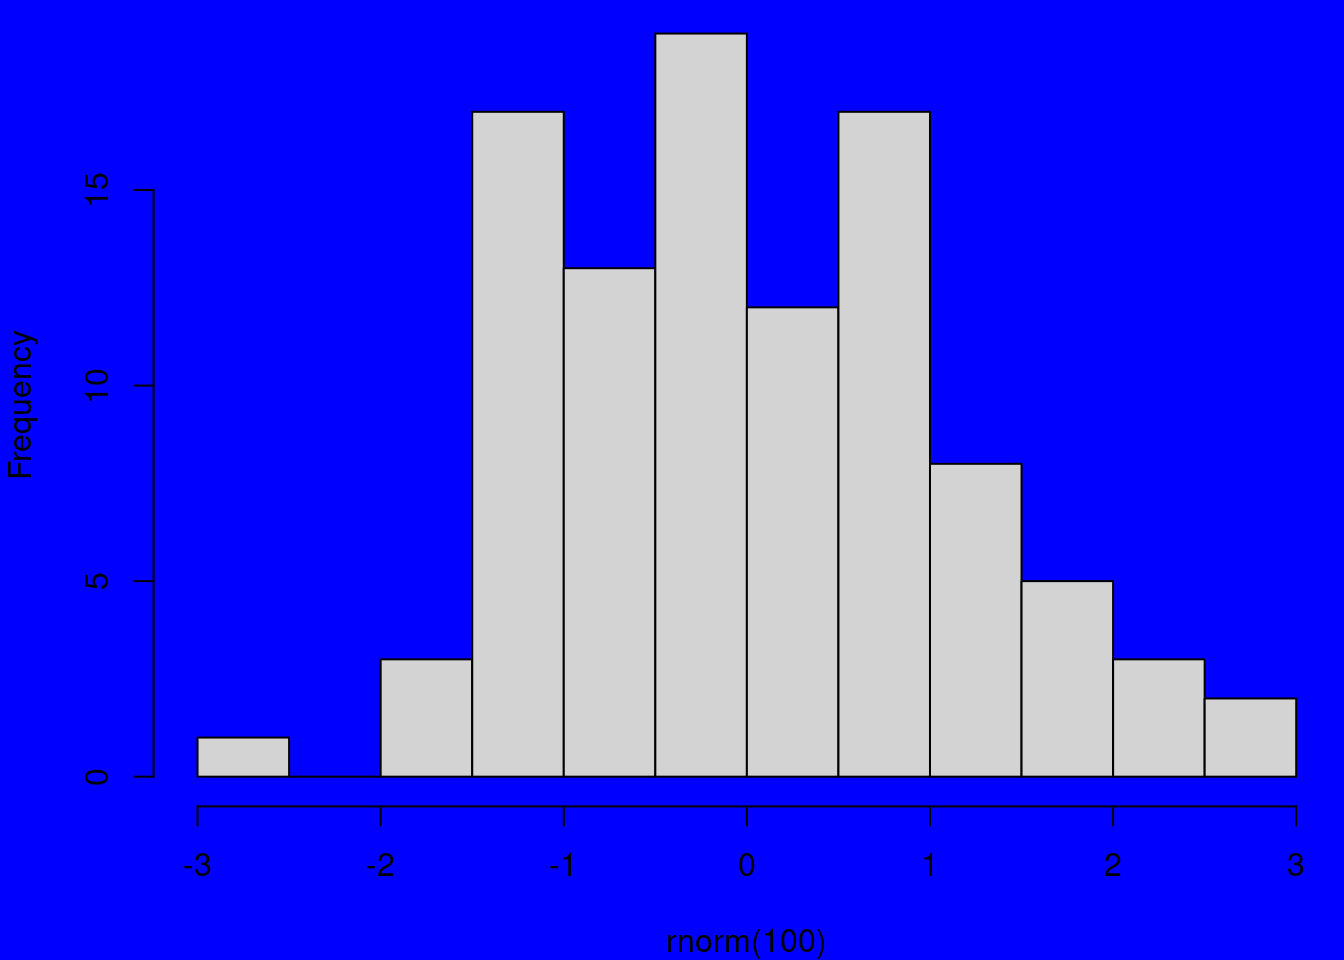
\includegraphics[width=1\linewidth,height=1\textheight,keepaspectratio]{knitr_files/figure-latex/myplot-1} \end{center}

\textbf{knitr} のフックは出力にテキストを挿入することにも使えます.
そのため, このタイプのフック関数は文字列を返す必要があります.
この機能はフックの能力を大いに広げます. \textbf{\texttt{rgl}}
パッケージを例に取りましょう. \textbf{rgl} によって生成された 3D
グラフを Markdown または HTML 文書に挿入したい時,
このタイプのフック関数を考える事になるでしょう (この例よりも洗練された
\texttt{hook\_rgl()} 関数が \textbf{\texttt{rgl}}
パッケージにあるので参照してください).

\begin{Shaded}
\begin{Highlighting}[numbers=left,,]
\NormalTok{knit\_hooks}\SpecialCharTok{$}\FunctionTok{set}\NormalTok{(}\AttributeTok{rgl =} \ControlFlowTok{function}\NormalTok{(before, options, envir) \{}
  \ControlFlowTok{if}\NormalTok{ (}\SpecialCharTok{!}\NormalTok{before) \{}
    \DocumentationTok{\#\# チャンクコードが評価された後の処理}
    \ControlFlowTok{if}\NormalTok{ (}\FunctionTok{rgl.cur}\NormalTok{() }\SpecialCharTok{==} \DecValTok{0}\NormalTok{) \{}
      \FunctionTok{return}\NormalTok{()}
\NormalTok{    \} }\CommentTok{\# アクティブなデバイスがないかどうか}
\NormalTok{    name }\OtherTok{\textless{}{-}} \FunctionTok{paste0}\NormalTok{(options}\SpecialCharTok{$}\NormalTok{fig.path, options}\SpecialCharTok{$}\NormalTok{label, }\StringTok{".png"}\NormalTok{)}
    \FunctionTok{rgl.snapshot}\NormalTok{(name, }\AttributeTok{fmt =} \StringTok{"png"}\NormalTok{)}
    \FunctionTok{return}\NormalTok{(}\FunctionTok{paste0}\NormalTok{(}\StringTok{"![rgl plot]("}\NormalTok{, name, }\StringTok{")}\SpecialCharTok{\textbackslash{}n}\StringTok{"}\NormalTok{))}
\NormalTok{  \}}
\NormalTok{\})}
\end{Highlighting}
\end{Shaded}

そしてコードチャンクはこのようになります.

\begin{verbatim}
```{r, fancy-rgl, rgl=TRUE}
library(rgl)  # 用例は ?plot3d から
open3d()
x = sort(rnorm(1000)); y = rnorm(1000); z = rnorm(1000) + atan2(x,y)
plot3d(x, y, z, col = rainbow(1000))
```
\end{verbatim}

Markdown の場合 \texttt{!{[}rgl\ plot{]}(fancy-rgl.png)}
と出力されているでしょう.

要約すると:

\begin{enumerate}
\def\labelenumi{\arabic{enumi}.}
\tightlist
\item
  フックは \texttt{knit\_hooks} で,
  \texttt{knit\_hooks\$set(foo\ =\ FUN)} という構文で設定されます
\item
  あるチャンクで \texttt{foo} というチャンクオプションが \texttt{NULL}
  以外の値をとる場合, このフック関数 \texttt{FUN} が実行されます.
\item
  フックはチャンクの直前と直後に実行できます
\item
  フックによって返される文字列は修正が加えられることなく出力ブロックに書き出されます.
\end{enumerate}

さらなる用例は
\href{https://github.com/yihui/knitr-examples/blob/master/045-chunk-hook.md}{045-chunk-hook.md}
(\href{https://github.com/yihui/knitr-examples/blob/master/045-chunk-hook.Rmd}{source})
を参照してください.

\hypertarget{ux51faux529bux30d5ux30c3ux30af}{%
\section{出力フック}\label{ux51faux529bux30d5ux30c3ux30af}}

出力フックはチャンクからの\textbf{生の}出力をカスタマイズし洗練するために使います.
様々な種類の出力に対処するための 8つの出力フック関数が存在します.

\begin{itemize}
\tightlist
\item
  \textbf{\texttt{source}}: ソースコード
\item
  \textbf{\texttt{output}}: 通常の R の出力で, 警告文, メッセージ文,
  エラー文を除くもの (つまり, 通常の R
  ターミナルで出力されていたものです)
\item
  \textbf{\texttt{warning}}: \texttt{warning()} による警告文
\item
  \textbf{\texttt{message}}: \texttt{message()} によるメッセージ文
\item
  \textbf{\texttt{error}}: \texttt{stop()} によるエラー文
  (コードチャンクとインライン R コードの両方に適用されます)
\item
  \textbf{\texttt{plot}}: 出力されるグラフ
\item
  \textbf{\texttt{inline}}: インライン R コードの出力
\item
  \textbf{\texttt{chunk}}: チャンクの全ての出力
  (つまりその前のフックにも生み出されたもの)
\item
  \textbf{\texttt{document}}: 文書全体の出力 (デフォルトでは
  \texttt{base::identity} が適用されます)
\end{itemize}

これらのフックは全て \texttt{function(x,\ options)} という形式をとります
(例外として, \texttt{inline} と \texttt{document} のフックのみ引数は
\texttt{x} の1つです), \texttt{x} が出力の文字列で, \texttt{options}
が現在のチャンクのオプションのリストです.
出力フックに関する情報と用例をさらに詳しく知りたい場合は
\href{https://bookdown.org/yihui/rmarkdown-cookbook/output-hooks.html}{\emph{R
Markdown Cookbook}} を参考にしてください.

以下は \texttt{error} フックの用例になります.
\href{https://rmarkdown.rstudio.com}{R Markdown} 上で,
エラー文に対して追加で整形処理をするフックです.

\begin{Shaded}
\begin{Highlighting}[numbers=left,,]
\NormalTok{knitr}\SpecialCharTok{::}\NormalTok{knit\_hooks}\SpecialCharTok{$}\FunctionTok{set}\NormalTok{(}\AttributeTok{error =} \ControlFlowTok{function}\NormalTok{(x, options) \{}
  \FunctionTok{paste}\NormalTok{(}\FunctionTok{c}\NormalTok{(}
    \StringTok{\textquotesingle{}}\SpecialCharTok{\textbackslash{}n\textbackslash{}n}\StringTok{:::\{style="color:Crimson; background{-}color: SeaShell;"\}\textquotesingle{}}\NormalTok{,}
    \FunctionTok{gsub}\NormalTok{(}\StringTok{"\^{}\#\# Error"}\NormalTok{, }\StringTok{"**Error**"}\NormalTok{, x),}
    \StringTok{":::"}
\NormalTok{  ), }\AttributeTok{collapse =} \StringTok{"}\SpecialCharTok{\textbackslash{}n}\StringTok{"}\NormalTok{)}
\NormalTok{\})}
\end{Highlighting}
\end{Shaded}

このようなチャンクでフックの動作をテストします

\begin{verbatim}
```{r, error=TRUE}
1 + "a"
```
\end{verbatim}

\textbf{Error} in 1 + ``a'': 二項演算子の引数が数値ではありません

デフォルトではチャンクフックは空ですが,
出力フックはデフォルト設定があり, 以下のようにしてリセットできます.

\begin{Shaded}
\begin{Highlighting}[numbers=left,,]
\NormalTok{knitr}\SpecialCharTok{::}\NormalTok{knit\_hooks}\SpecialCharTok{$}\FunctionTok{restore}\NormalTok{()}
\end{Highlighting}
\end{Shaded}

\begin{infobox}{caution}
\textbf{訳注}

R Markdown の場合,
基本的な出力フォーマットにもデフォルトでフックが定義されており,
処理内容によっては予期せぬ結果になることがあるため, 単純な上書きや
\texttt{\$restore()} は意図しない動作につながることがあります. 詳細は
``R Markdown Cookboox''
\href{https://bookdown.org/yihui/rmarkdown-cookbook/output-hooks.html}{Ch.
12}\footnote{翻訳版:
  \url{https://gedevan-aleksizde.github.io/rmarkdown-cookbook/output-hooks.html}}
を確認ください.

\end{infobox}

本パッケージは出力を異なる部品にわけてそれぞれにデフォルトのフックを設定し,
さらに LaTeX, HTML, Jekyll
といった異なる出力フォーマットごとに用意しています. \texttt{render\_*()}
という一連の関数群は, 例えば \texttt{render\_latex()},
\texttt{redner\_html()}, など出力フォーマットごとにそれぞれ異なる,
組み込みの出力フックを提供するためにあります.
出力フックはドキュメント内で設定すべきですが, \texttt{knitr::knit()}
が文書を処理する前にフックを設定したなら \texttt{render\_*()}, たとえば
\texttt{render\_markdown()}, \texttt{render\_html()}
を最初に呼び出さなければなりません. \texttt{hooks\_markdown()} などの
\texttt{hooks\_*()} 関数で,
設定を変えることなくこれらの出力フックにアクセスすることができます.

以降は各フォーマットでの詳細を記します.

\hypertarget{latex-render_latex}{%
\subsection{\texorpdfstring{LaTeX:
\texttt{render\_latex()}}{LaTeX: render\_latex()}}\label{latex-render_latex}}

出力ファイルタイプが LaTeX の場合,
デフォルトのフックはほとんどのチャンク出力を \texttt{verbatim}
環境で囲んで出力し, \texttt{inline}
出力における数値を指数表記で出力します (詳細は
\protect\hyperlink{output}{チャンク出力の制御}のデモを参照してください).
\texttt{plot}, \texttt{chunk} フックはより複雑な処理をしています.

\begin{itemize}
\tightlist
\item
  デフォルトでは \texttt{plot}
  フックは出力の信頼性を維持するため多くの要因に影響されます.

  \begin{itemize}
  \tightlist
  \item
    たとえばグラフィックデバイスが \texttt{tikz} ならば,
    \texttt{\textbackslash{}input\{\}}
    コマンドが使われますし\footnote{訳注: tikz の画像は LaTeX
      ソースコードで記述されるため, \texttt{\textbackslash{}input\{\}}
      でテキストファイルとして読み込む必要があります.},
    それ以外では通常は \texttt{\textbackslash{}includegraphics\{\}}
    コマンドが使われます.
  \item
    \texttt{out.width}, \texttt{out.height} オプションに依存して,
    フックはグラフのサイズをリセットします (たとえば
    \texttt{\textbackslash{}includegraphics{[}width=.8\textbackslash{}textwidth{]}\{file\}}
    のように). 1つのチャンクに複数のグラフがある場合,
    \texttt{fig.show=\textquotesingle{}hold\textquotesingle{}}
    を設定するとともに,
    複数の画像を適切なサイズで横に並べて表示できるように設定できます
    (たとえば \texttt{.45\textbackslash{}textwidth}\footnote{訳注:
      本文幅の45\%} とすれば横に2つのグラフを並べられます).
  \item
    tikz のグラフは \texttt{\textbackslash{}input\{\}} で挿入するため,
    このやり方は正しくありませんが, チャンクオプション
    \texttt{resize.width} と \texttt{resize.height} は複数の tikz
    グラフを横に並べることができます
    (\texttt{\textbackslash{}resizebox\{resize.width\}\{resize.height\}\{file.tikz\}}
    という書き方によって. もしいずれかのオプションが \texttt{NULL} なら
    \texttt{!} で置き換えられます. 詳細は LaTeX パッケージの
    \texttt{graphicx} のドキュメントを参照してください).
    このフック関数によってユーザーは自動レポート生成の全能力を使いこなせます
    ---
    単一チャンクの複数グラフとグラフのサイズの設定が可能になるだけでなく,
    base R のグラフィックスや grid 系のグラフィックス (例:
    \textbf{ggplot2}),
    あるいはグリッド系のグラフを並べて表示することもできます ---
    この機能がなかったら, R
    で1つのウィンドウにこういった複数のグラフを1つにまとめるのがどんなに難しいことか考えても見てください\footnote{訳注:
      現在は \texttt{patchwork} や \texttt{cowplot}
      パッケージなどの登場により,
      そこまで難しいことではなくなりつつあります}.
  \item
    グラフのアラインを決めるために \texttt{fig.align}
    には4つの値が用意され (\texttt{default}, \texttt{left},
    \texttt{right}, \texttt{center}), 簡単に画像を中央揃えにできます
    (\texttt{fig.align=\textquotesingle{}center\textquotesingle{}}
    によって).
  \end{itemize}
\item
  デフォルトの \texttt{chunk}
  フックは主にチャンクの装飾に使われています.

  \begin{itemize}
  \tightlist
  \item
    LaTeX の \texttt{framed} パッケージがユーザーの TeX
    ソフトウェアパッケージ (TeXLive か MikTeX か他の何か\footnote{訳注:
      あるいは Yihui 氏による TinyTeX とか})
    にインストールされているなら, \texttt{chunk}
    フックはカスタマイズした背景色 (デフォルトでは薄灰色) にした
    \texttt{kframe} 環境に全ての出力を挿入することで,
    チャンクの視認性を向上させます (他の地の文よりも強調されますが,
    とても目立つというほどでもないはずです).
  \item
    最後に, 全ての出力が \texttt{knitrout} 環境で囲まれます.
    この環境はユーザーが LaTeX で再定義できます.
  \end{itemize}
\end{itemize}

\hypertarget{sweave-render_sweave}{%
\subsection{\texorpdfstring{Sweave:
\texttt{render\_sweave()}}{Sweave: render\_sweave()}}\label{sweave-render_sweave}}

ソースコードを \texttt{Sinput} 環境に挿入し, その出力を
\texttt{Sioutput} 環境に挿入し, そしてチャンク全体を \texttt{Schunk}
環境に挿入します. このテーマの使用にはスタイルファイル
\texttt{Sweave.sty} か,
少なくともこれら3つの環境を定義することが必要です.

\hypertarget{listings-render_listings}{%
\subsection{\texorpdfstring{Listings:
\texttt{render\_listings()}}{Listings: render\_listings()}}\label{listings-render_listings}}

Sweave 同様に,
\href{https://github.com/yihui/knitr/blob/master/inst/misc/Sweavel.sty}{\texttt{Sweavel.sty}}
が使用されます.

\hypertarget{html-render_html}{%
\subsection{\texorpdfstring{HTML:
\texttt{render\_html()}}{HTML: render\_html()}}\label{html-render_html}}

HTML ファイルに書き出すにあたって, フックは出力を自動で調整します.
基本的にチャンクによる出力はクラス付きの \texttt{div}
レイヤーに挿入されます. たとえば, ソースコードは
\texttt{\textless{}div\ class="knitr\ source"\textgreater{}\textless{}/div\textgreater{}},
チャンク全体は
\texttt{\textless{}pre\textgreater{}\textless{}/pre\textgreater{}} に,
インラインの出力は
\texttt{\textless{}code\ class="knitr\ inline"\textgreater{}\textless{}/code\textgreater{}}
に書き出されます\footnote{訳注: R Markdown
  では最終的に出力されるHTMLはさらに pandoc
  などの処理を経由しているため, これとは異なります}.

\hypertarget{markdown-render_markdown}{%
\subsection{\texorpdfstring{Markdown:
\texttt{render\_markdown()}}{Markdown: render\_markdown()}}\label{markdown-render_markdown}}

ソースコードとその出力はスペース4つでインデントされます. GitHub Flavored
Markdown のため, ソースコードは
\texttt{\textasciigrave{}\textasciigrave{}\textasciigrave{}r} と
\texttt{\textasciigrave{}\textasciigrave{}\textasciigrave{}}
の間に挿入され, 出力部分は
\texttt{\textasciigrave{}\textasciigrave{}\textasciigrave{}} と
\texttt{\textasciigrave{}\textasciigrave{}\textasciigrave{}}
の間に挿入されます.

\hypertarget{jekyll-render_jekyll}{%
\subsection{\texorpdfstring{Jekyll:
\texttt{render\_jekyll()}}{Jekyll: render\_jekyll()}}\label{jekyll-render_jekyll}}

このサイト\footnote{訳注: オリジナルが掲載されている Yihui
  氏のサイトのこと}を構築するために, Jykell
用に特別にいくつかのフックを用意する必要がありました.
これらは実際かなり単純なものです. R
ソースコードはハイライト環境に挿入し言語を \texttt{r} に設定する,
残りの出力部分は \texttt{text} 言語に設定したハイライト環境
(ほとんど何もハイライトしない) に挿入するだけです. 現在, グラフは
Markdown の構文に従って書き出されます.

\hypertarget{restructuredtext-render_rst}{%
\subsection{\texorpdfstring{reStructuredText:
\texttt{render\_rst()}}{reStructuredText: render\_rst()}}\label{restructuredtext-render_rst}}

コードは \texttt{::} の後に挿入され, スペース4個でインデントされるか,
\texttt{sourcecode} ディレクティブに挿入されます.

\hypertarget{ux30aaux30d7ux30b7ux30e7ux30f3ux30d5ux30c3ux30af}{%
\section{オプションフック}\label{ux30aaux30d7ux30b7ux30e7ux30f3ux30d5ux30c3ux30af}}

他のチャンクオプションの値に応じて別のチャンクオプションの値を変えたいとき,
\texttt{opts\_hooks} をつかってそれを実行することがあるかもしれません.
オプションフックは対応するチャンクオプションの値が \texttt{NULL}
以外であるときに実行されます. たとえば \texttt{fig.width} を常に
\texttt{fig.height} 以上の値に調整することができます.

\begin{Shaded}
\begin{Highlighting}[numbers=left,,]
\NormalTok{knitr}\SpecialCharTok{::}\NormalTok{opts\_hooks}\SpecialCharTok{$}\FunctionTok{set}\NormalTok{(}\AttributeTok{fig.width =} \ControlFlowTok{function}\NormalTok{(options) \{}
  \ControlFlowTok{if}\NormalTok{ (options}\SpecialCharTok{$}\NormalTok{fig.width }\SpecialCharTok{\textless{}}\NormalTok{ options}\SpecialCharTok{$}\NormalTok{fig.height) \{}
\NormalTok{    options}\SpecialCharTok{$}\NormalTok{fig.width }\OtherTok{\textless{}{-}}\NormalTok{ options}\SpecialCharTok{$}\NormalTok{fig.height}
\NormalTok{  \}}
\NormalTok{  options}
\NormalTok{\})}
\end{Highlighting}
\end{Shaded}

\texttt{fig.width} は \texttt{NULL} になることがないため,
このフック関数は常にチャンクの直前の,
チャンクオプションが確認される前に実行されます.
以下のコードチャンクは上記のフックを設定することで, \texttt{fig.width}
の実際の値は初期値の \texttt{5} の代わりに \texttt{6} が適用されます.

\begin{Shaded}
\begin{Highlighting}[]
\StringTok{\textasciigrave{}\textasciigrave{}\textasciigrave{}}\AttributeTok{\{r fig.width = 5, fig.height = 6\}}
\AttributeTok{plot(1:10)}
\StringTok{\textasciigrave{}\textasciigrave{}\textasciigrave{}}
\end{Highlighting}
\end{Shaded}

\begin{center}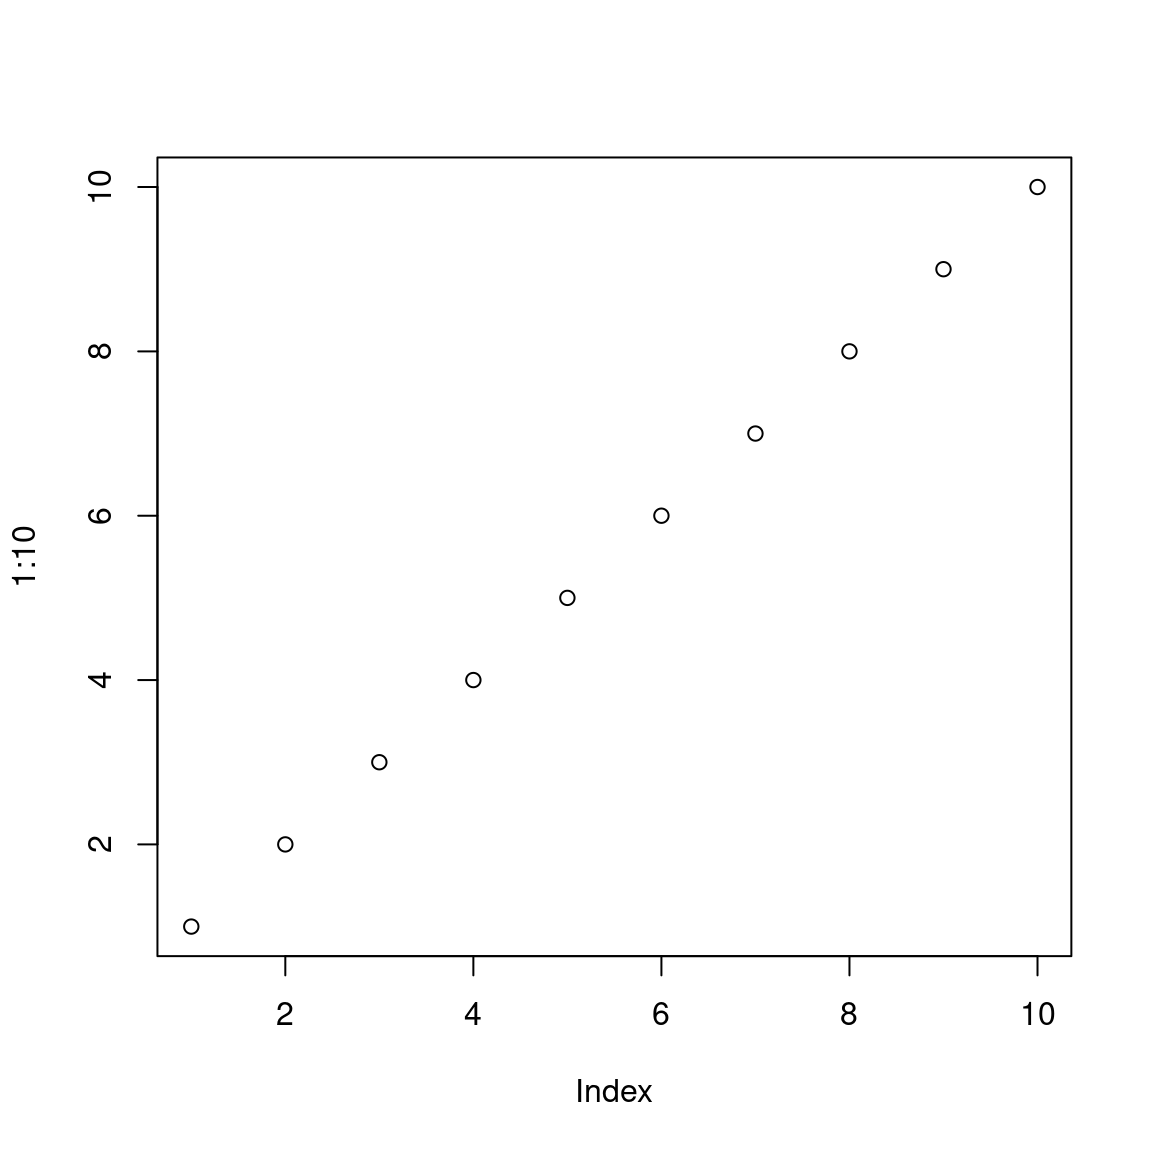
\includegraphics[width=1\linewidth,height=1\textheight,keepaspectratio]{knitr_files/figure-latex/unnamed-chunk-2-1} \end{center}

訳注: \texttt{knit\_hooks} 同様に, \texttt{opts\_hooks} にも
\texttt{restore()} メソッドが用意されています.

\hypertarget{examples}{%
\chapter{使用例}\label{examples}}

ソースと出力のデモ

オリジナルのページ: \url{https://yihui.org/knitr/demos/}

オリジナルの更新日: 2017-02-03

\begin{center}\rule{0.5\linewidth}{0.5pt}\end{center}

\begin{infobox}{memo}
\textbf{訳注}: 現在は knitr の主な利用場面は R Markdown
との併用だと思うので, それらと関係の薄いページは翻訳していません. また,
編集上の問題から,
ここで挙げられているページのうち翻訳済みのものは全てナビゲーションバーの「用例」パートでもリンクされています.

\end{infobox}

Github の \href{https://github.com/yihui/knitr-examples}{knitr-examples}
はより豊富なコレクションになっています.
このページはむしろドキュメント用途として作られています.
他のユーザーによる
\protect\hyperlink{showcase}{\textbf{knitr}のショーケース}
を見ることもできます.

\begin{itemize}
\tightlist
\item
  2011-12-03 \href{https://yihui.org/knitr/demo/minimal}{(未翻訳)
  Minimal examples - Examples for Rnw, Markdown, HTML and LaTeX}
\item
  2011-12-04 \protect\hyperlink{cache}{キャッシュ -
  キャッシュ機能の使用例について}
\item
  2011-12-05 \protect\hyperlink{manual}{マニュアル -
  パッケージマニュアルについて}
\item
  2011-12-06 \href{https://yihui.org/knitr/demo/lyx}{(未翻訳) LyX -
  Using knitr with LyX}
\item
  2011-12-07
  \href{https://yihui.org/knitr/demo/externalization}{(未翻訳) Code
  Externalization - Use an external R script with your document}
\item
  2011-12-08 \href{https://yihui.org/knitr/demo/beamer}{(未翻訳) Beamer
  - Using knitr in beamer slides}
\item
  2011-12-09 \protect\hyperlink{graphics}{グラフィックス -
  \textbf{knitr} におけるグラフィックスの力について}
\item
  2011-12-10 \protect\hyperlink{listings}{\texttt{Listings} -
  \texttt{listings} と \texttt{knitr} の併用}
\item
  2012-01-14 \protect\hyperlink{reference}{チャンク参照/マクロ -
  チャンクの再利用方法}
\item
  2012-01-18 \href{https://yihui.org/knitr/demo/child}{(未翻訳) Child
  documents - Input child files into the main document}
\item
  2012-01-22 \href{https://yihui.org/knitr/demo/vignette}{(未翻訳)
  Package vignettes - How to build package vignettes with knitr}
\item
  2012-01-25 \protect\hyperlink{output}{チャンク出力の制御 -
  チャンクの6種類の出力とインライン出力を操作する}
\item
  2012-01-26 \href{https://yihui.org/knitr/demo/stitch}{(未翻訳) Quick
  reporting - Build a report based on an R script}
\item
  2012-02-01 \href{https://yihui.org/knitr/demo/org}{(未翻訳) Org-mode -
  Use knitr in Org-mode}
\item
  2012-02-02 \href{https://yihui.org/knitr/demo/rstudio}{(未翻訳)
  RStudio - knitr support in RStudio}
\item
  2012-02-11 \href{https://yihui.org/knitr/demo/pretty}{(未翻訳) Pretty
  printing - Print highlighted source code of a function}
\item
  2012-02-12 \href{https://yihui.org/knitr/demo/upload}{(未翻訳) Upload
  images - Publish images from chunks in the web}
\item
  2012-02-24 \href{https://yihui.org/knitr/demo/sweave}{(未翻訳) Sweave
  - Transition from Sweave to knitr}
\item
  2012-02-27 \href{https://yihui.org/knitr/demo/eclipse}{(未翻訳)
  Eclipse - Configure Eclipse to work with knitr}
\item
  2012-02-29 \protect\hyperlink{framed}{\texttt{framed} パッケージ -
  \textbf{knitr} における LaTeX のデフォルトスタイル}
\item
  2012-03-16 \protect\hyperlink{editors}{\texttt{knitr} のエディタ -
  Emacs, TeX Maker, TeXShop, WinEdt, そして TextMate などについて}
\item
  2012-05-01 \href{https://yihui.org/knitr/demo/slides}{(未翻訳) HTML5
  slides - making HTML5 slides with pandoc and knitr}
\item
  2012-05-04 \href{https://yihui.org/knitr/demo/engines}{(未翻訳)
  Language engines - Use other languages in knitr}
\item
  2012-11-09 \href{https://yihui.org/knitr/demo/javascript}{(未翻訳)
  JavaScript - Combine R and JS applications like D3}
\item
  2013-02-10 \href{https://yihui.org/knitr/demo/wordpress}{(未翻訳)
  WordPress - Publish blog posts from R + knitr to WordPress}
\item
  2013-03-06 \href{https://yihui.org/knitr/demo/pandoc}{(未翻訳) Pandoc
  - Convert Markdown to other formats via Pandoc}
\item
  2013-03-11 \protect\hyperlink{showcase}{\texttt{knitr} のショーケース
  - ユーザーたちによる使用例}
\end{itemize}

\hypertarget{FAQs}{%
\chapter{よくある質問 (FAQ)}\label{FAQs}}

オリジナルのページ: \url{https://yihui.org/knitr/faq/}

オリジナルの更新日: 2017-02-17

\begin{center}\rule{0.5\linewidth}{0.5pt}\end{center}

この FAQ は \href{https://github.com/yihui/knitr/issues}{issues} や私
(Yihui) のブログやEメールに届いた質問などを蓄積したものです.
個人的な考えとして, 私は FAQ という概念の大ファンでもありませんし, FAQ
はときとしてほとんどバグのようなものであると思っています.
ソフトウェアパッケージの作者は,
ユーザーがそんな質問を頻繁にする理由を考えるべきです
(ユーザーが全員愚かであるから, という考えには賛成できません).
少なくとも私は, 128件もの質問を1つ1つ読み返すほど忍耐強くありませんし,
これを読んでいるあなたにも同様のことをさせるつもりはありません.

\begin{enumerate}
\def\labelenumi{\arabic{enumi}.}
\tightlist
\item
  「\textbf{knitr}が動かないんだけど\ldots」

  \begin{itemize}
  \tightlist
  \item
    まず最初に, あなたの R パッケージ (\texttt{update.packages()}
    を使います) とたぶん R 本体も (ところで,
    現在のあなたの\href{https://cran.rstudio.com}{Rのバージョン}は何ですか?)
    更新してください. それから動くかどうかを確認してください.
    もしそれでも動かなかったら,「必要最低限の再現例 (minimal
    reprex)」のファイルと \texttt{library(knitr);\ sessionInfo()}
    の実行結果を \href{https://github.com/yihui/knitr/issues}{issue}
    に投稿してください.
  \end{itemize}
\item
  「パッケージのサイトの説明が役に立たないときはどこで質問するのがいいですか?」

  \begin{itemize}
  \tightlist
  \item
    何を質問したいかにもよりますが,
    以下のような選択肢があります\footnote{訳注: 英語が苦手な場合は,
      \href{https://ja.stackoverflow.com/}{Stack Oveflow 日本語版},
      または
      \href{https://r-wakalang.slack.com/messages/general/}{R-wakalang}
      などのコミュニティがあります}
    (特に最初の2つは私もよく巡回しています).

    \begin{itemize}
    \tightlist
    \item
      (推奨)
      \textbf{\href{http://stackoverflow.com/questions/tagged/knitr}{Stack
      Overflow}}: 一般的な質問 (より専門的で早い回答がつきます).
      \texttt{r} と \texttt{knitr} タグを忘れずにつけてください.
    \item
      \textbf{\href{https://github.com/yihui/knitr/issues}{Github
      issues}}: バグ報告と機能追加の要望のみにしてください.
    \item
      \textbf{\href{https://groups.google.com/group/knitr}{knitr mailing
      list}} または
      \textbf{\href{http://www.r-project.org/mail.html}{R-help}}
      のメーリングリスト: 一般的な質問とその回答が,
      一般公開されるEメールによってやりとりされます.
    \item
      \textbf{私の個人的なEメール}:
      本当にプライベートな問題でない限り\href{https://yihui.org/en/2017/08/so-gh-email/}{非推奨}です\footnote{訳注:
        リンク先の投稿を要約すると,
        Yihui氏個人で次から次へと来る質問をさばくのは限界があるし,
        オープンコミュニティは多くの回答者がいて既出の質問に対する答えも共有でき効率的だ,
        ということです}.
    \item
      \textbf{Twitter} (\href{http://twitter.com/xieyihui}{@xieyihui}):
      本当に簡単な問題だと確信があるなら.
    \end{itemize}
  \end{itemize}
\item
  「\textbf{knitr}
  のソースドキュメントを書くのに最適のエディタソフトは何ですか?」

  \begin{itemize}
  \tightlist
  \item
    初心者にとってはたぶん \href{https://www.rstudio.com}{RStudio}
    が良いです. \textbf{knitr} は \href{/knitr/demo/lyx/}{LyX},
    \href{http://ess.r-project.org/}{Emacs/ESS}, WinEdt, Tinn-R and
    や\protect\hyperlink{editors}{その他多くのエディタ}でサポートされています.
  \end{itemize}
\item
  「\texttt{\textgreater{}} とか \texttt{+}
  とかのプロンプト記号はどこへいったんですか?
  出力にこれがないと落ち着きません」

  \begin{itemize}
  \tightlist
  \item
    \href{https://yihui.org/en/2013/01/code-pollution-with-command-prompts/}{私はこれらが意味をなさないと考えている}ので,
    デフォルトではこれらは除去されています. R の本に
    \texttt{\textgreater{}} や \texttt{+}
    を載せるのを嫌う理由はこのようなものです: 本に書かれた R
    コードを読む際に,
    \textbf{こいつらは私の精神をめちゃくちゃにひねりちぎろうとし,
    私の両眼に流血を欲してきます}. マジで \texttt{1\ +\ 1} ではなく
    \texttt{\textgreater{}\ 1+1} という表記を読むのがお好みな奇特な方は,
    \protect\hyperlink{options}{チャンクオプション} の章にあるように
    \texttt{prompt} オプションで設定できます\footnote{訳注: Yihui
      氏がこれを嫌う理由はここでも簡潔に書かれています. R Markdown
      においては, それ以外の方法でもコードの装飾をカスタマイズできます.
      たとえばこの翻訳版でなされているようにコピーボタンや行番号をつけたりできます.}.
  \end{itemize}
\item
  「ワーキングディレクトリとはなんですか?
  コードチャンク内でワーキングディレクトリを変更できますか?」

  \begin{itemize}
  \tightlist
  \item
    あなたはそういうことをしないほうがよいです.
    ワーキングディレクトリは常に \texttt{getwd()} で分かります
    (出力ファイルは全てここに書き出されます) が,
    コードチャンクは入力ファイルがあった場所で評価しています. R
    コード実行中のワーキングディレクトリ変更は一般的に, よくない使い方
    (バッドプラクティス) です. 詳しくは issue
    \href{https://github.com/yihui/knitr/issues/38}{\#38}
    での議論をご覧ください. また, できることなら常に,
    絶対パスによるディレクトリ指定も回避するべきです.
    代わりに相対パス指定を使ってください.
    そのようなコードは再現性を損なうからです.
    ここまで言ってもまだコードチャンク内で \texttt{setwd}
    を使おうというのなら,
    新しく設定したワーキングディレクトリは指定したチャンクにのみ適用され,
    以降のコードチャンクでは本来のワーキングディレクトリに差し戻されることを留意してください.
  \end{itemize}
\item
  「出力された灰色の背景色ボックスが狭すぎます.」

  \begin{itemize}
  \tightlist
  \item
    それはボックスが狭すぎるからではありません.
    ボックス幅は現在行の幅が適用されます.
    つまりあなたの出力のほうが広すぎるのです.
    ページのマージンを超えるような出力を避けるため, もっと小さな
    \texttt{width} オプションを設定してください (例:
    \texttt{options(width\ =\ 60)},
    詳細は\href{https://github.com/yihui/knitr-examples/blob/master/038-output-width.Rnw}{example
    038} を参照してください.)
  \end{itemize}
\item
  「コードチャンクにリテラルや生のコードを書く方法は?
  たとえばパースせずにコードチャンクを書きたいです.
  チュートリアルに便利だと思います.」

  \begin{itemize}
  \tightlist
  \item
    チャンクヘッダを破壊する必要があります. たとえば
    \texttt{\textasciigrave{}\textasciigrave{}\textasciigrave{}\{r\}\textasciigrave{}r\textquotesingle{}\textquotesingle{}\textasciigrave{}\ \textasciigrave{}\textasciigrave{}\textasciigrave{}}
    のように, チャンクヘッダの前後に空の文字列を加えます(issues
    \href{https://github.com/yihui/knitr/issues/443}{\#443}).
    あるいはチャンクヘッダに\href{https://ja.wikipedia.org/w/index.php?title=\%E3\%82\%BC\%E3\%83\%AD\%E5\%B9\%85\%E3\%82\%B9\%E3\%83\%9A\%E3\%83\%BC\%E3\%82\%B9\&oldid=78849992}{ゼロ幅スペース}を追加します.
    詳細は \href{https://github.com/yihui/knitr-examples}{example 065}
    を見てください.
  \item
    インラインの R コードでは \texttt{knitr::inline\_expr()}
    を使うことになるでしょう (\textbf{knitr} ver. 1.8
    以降で使用できます). R Markdown で書いている場合は,
    あるトリックを使えます. \texttt{\textasciigrave{}r}
    \textbf{直後に}改行を入れ
    (実際にやるときは直後にスペースを入れないでください),
    二重のバッククオート (バックティック)
    のペアでインラインの評価式全体を囲みます.
    例えば以下のようになります. この挙動の説明に興味があるなら
    \href{https://yihui.org/en/2017/11/knitr-verbatim-code-chunk/}{このページ}
    を見てください (訳注: 未翻訳).
  \end{itemize}
\end{enumerate}

\textbf{訳注}: ソースコードでの記述

\begin{verbatim}
````
```{r, eval=TRUE}`r ''`
1 + 1
```
````
\end{verbatim}

実際に表示されるもの

\begin{verbatim}
```{r, eval=TRUE}
1 + 1
```
\end{verbatim}

インライン式では以下のようになります

\begin{verbatim}
ここに生のインラインR評価式を出力: `` `r
1+1` ``.
\end{verbatim}

ここに生のインラインR評価式を出力:
\texttt{\textasciigrave{}r\ 1+1\textasciigrave{}}.

\begin{enumerate}
\def\labelenumi{\arabic{enumi}.}
\setcounter{enumi}{7}
\tightlist
\item
  「何かお役に立てることはありますか?」

  \begin{itemize}
  \tightlist
  \item
    \href{https://paypal.me/YihuiXie}{paypal} でドネートできますし,
    たのしい GIF
    アニメを私に\href{https://twitter.com/xieyihui}{ツイート}したり,
    Github で \textbf{knitr}
    のリポジトリをフォークしたりコードの改善に貢献したりできます.
  \item
    パッケージや \href{http://amzn.com/1498716962}{knitr book}
    を引用してください. R で
    \texttt{citation(\textquotesingle{}knitr\textquotesingle{})}
    をしてみてください.
  \end{itemize}
\item
  「このドキュメントの修正や小さな変更を投稿するにはどうすればいいですか?」

  \begin{itemize}
  \tightlist
  \item
    R パッケージを修正したい場合は
    \href{https://github.com/yihui/knitr}{リポジトリ} へ移動し,
    ツールバー右上の Edit ボタンを押します. それから必要な修正をします.
    投稿の概要を書いて, \textbf{Propose file change} をクリックして,
    プルリクエストを投稿してください.
  \item
    このウエブサイト (\url{https://yihui.org/knitr})
    上の修正や変更提案は, ページ左側の \texttt{Edit\ this\ page}
    を押して, あとは Github の手順に従ってください\footnote{訳注:
      原典ではなくこの翻訳版に対する修正提案は
      \url{https://github.com/Gedevan-Aleksizde/knitr-doc-ja}
      で受け付けています}.
  \end{itemize}
\end{enumerate}

\hypertarget{part-ux7528ux4f8b}{%
\part{用例}\label{part-ux7528ux4f8b}}

\hypertarget{editors}{%
\chapter*{\texorpdfstring{\texttt{knitr}
のエディタ}{knitr のエディタ}}\label{editors}}
\addcontentsline{toc}{chapter}{\texttt{knitr} のエディタ}

Emacs, TeX Maker, TeXShop, WinEdt, そして TextMate などについて

オリジナルの記事: \url{https://yihui.org/knitr/demo/editors/}

オリジナルの更新日: 2012-03-16

\begin{center}\rule{0.5\linewidth}{0.5pt}\end{center}

\begin{infobox}{tip}
\textbf{訳注}: このページは R Markdown ではなく, Rnw を想定した説明です.
R Markdown は基本的に RStudio での編集が最も使いやすいと思われます.

\end{infobox}

私は以前 \href{$lyx}{Lyx} (未翻訳), \href{$RStudio}{RStudio} (未翻訳)
\href{$org}{Emacs Org-mode} (未翻訳), \href{$ecripse}{Ecripse} (未翻訳)
について書きました. その他にも,
\href{http://www.xm1math.net/texmaker/}{Texmaker} や Windt
といったエディタで \textbf{knitr} を使うことができます. ポイントは R
を呼び出して \textbf{knitr} パッケージを読み込み, それから
\texttt{knit()}または \texttt{knit2pdf()} を呼び出すことです.

\hypertarget{texmaker}{%
\section*{Texmaker}\label{texmaker}}
\addcontentsline{toc}{section}{Texmaker}

\texttt{User\ -\/-\textgreater{}\ User\ Commands\ -\/-\textgreater{}\ Edit\ User\ Commands}
から, Rnw 文書を処理するためのカスタムコマンドを定義できます.

\begin{figure}

{\centering \includegraphics[width=1\linewidth,height=1\textheight,keepaspectratio]{ddIBH} 

}

\caption{Texmaker でユーザーコマンドを定義する}\label{fig:demo-def-user-command-texmaker}
\end{figure}

Rの実行ファイルパスが \texttt{PATH} 環境変数にない場合, 上記のコマンドに
\texttt{Rscript.exe} のフルパスを書く必要があります. こんなかんじに:

\begin{Shaded}
\begin{Highlighting}[]
\StringTok{"C:/Program Files/R/R{-}2.14.2/bin/Rscript.exe"} \AttributeTok{{-}e} \StringTok{"knitr::knit2pdf(\textquotesingle{}\%.Rnw\textquotesingle{})"}
\end{Highlighting}
\end{Shaded}

\texttt{Rscript.exe} の場所さえ知っていれば, R を開いて
\texttt{R.home(\textquotesingle{}bin\textquotesingle{})}
を実行すれば見つけられます. そうすればどんな Rnw 文書ファイルに対しても,
この \texttt{knitr} コマンドでコンパイルすることができます.

\begin{figure}

{\centering \includegraphics[width=1\linewidth,height=1\textheight,keepaspectratio]{xKoeT} 

}

\caption{Texmaker で knitr コマンドでコンパイルする}\label{fig:demo-compile-texmaker}
\end{figure}

文書をコンパイルするには左向きの矢印をクリックし, PDF
を表示するのに右矢印をクリックします. もちろん上記の設定は Windows
のものですが, 他のシステムでも同じ要領です. \texttt{Rscript.exe} を
\texttt{Rscript} に置き換えてください (実際は Windows 環境でも
\texttt{Rscript} が使えます).

\hypertarget{texstudio}{%
\section*{TeXStudio}\label{texstudio}}
\addcontentsline{toc}{section}{TeXStudio}

一例として, 基本的には Texmaker と同様に設定することができます (Henrik
Nyhus と
\href{https://twitter.com/MathBioPaul/status/691446297304272897}{Paul J.
Hurtado} に感謝)

\begin{figure}

{\centering \includegraphics[width=1\linewidth,height=1\textheight,keepaspectratio]{VFcvTUB} 

}

\caption{TeXStudio での knitr}\label{fig:demo-editor-texstudio}
\end{figure}

上級者向けオプション (左下) を解放すれば, 下部に
\texttt{Commands\ (\$PATH)} が現れるでしょう. ここに \texttt{R}
フォルダのパスを入力できます (例: 引用符なしで
\texttt{C:\textbackslash{}Program\ Files\textbackslash{}R\textbackslash{}R-3.3.2\textbackslash{}bin\textbackslash{}x64}).
それからユーザーコマンド (そして他のコマンドからも呼び出せる) に
\texttt{Rscript.exe\ -e\ "knitr::knit2pdf(\textquotesingle{}\%.Rnw\textquotesingle{})"}
とするだけです.

いつでもこのコマンドを実行できます (ホットキーは Alt-Shift-F1) し,
サイレントモードでも knitr で PDF を生成できます. F7
キーでいつでも表示されている PDF を更新できます. 代わりの方法として,
コマンドの末尾に \texttt{\textbar{}\ txs:///view-pdf}
を追加する方法があります.
これはあるコマンドの実行後に実行する別のコマンドを分けるパイプ記号です.
よって基本的に F7 を押すだけで事足りるようになります.

しかし, もし BibLaTeX のような文献引用パッケージを使うならば,
まだかなり非効率です. コンパイルの前に bib
ファイルの処理を手動で行う必要があり,
よって最低でも2回手動でコンパイルする必要があり
(そしてあなたは何回必要か正確に分からないでしょう).
その間に不要なビューアの呼び出しが発生します. TeXstudio
は文献処理ツール起動したりコンパイルしたり,
それらを繰り返すのに優れていますが, ビルドと閲覧 (F5)
を何度も押す度にこれが必要になり, そこでデフォルトのコンパイラを
\texttt{Rscript.exe\ -e\ "knitr::knit2pdf(\textquotesingle{}\%.Rnw\textquotesingle{})"}
で置き換えることで \textbf{knitr} を使用し続けられるわけです (\texttt{R}
フォルダを \texttt{\$PATH} に設定している前提です). その隣の ``Repeat
contained compilation commands''
が押されたままであることを確認してください.

もちろん, これならば少なくとも F5 (または F6) を押すだけで TeXstudio
デフォルトの標準の LaTeX コンパイラの代わりに \texttt{knitr}
が実行されます. この方法のおそらく唯一の欠点は, ほとんどの人にとって
LaTeX コードのデバッグがいっそう困難になることです.
ほとんどのエラーが「\texttt{texify.exe} ``had status
1''」という曖昧な警告に置き換わってしまうことです
(ユーザーコマンド経由で \textbf{knitr}
を実行するのではこれは改善できません).
そのような状況でもログファイルも時には有用ですが, ログファイルは
\texttt{.Rnw} ファイルではなく \textbf{knitr} の生成した \texttt{.tex}
を参照するので,
このファイルを開いてどこがおかしいのかを見つけようとする必要があります.

しかし物事の全体で見れば, TeXstudio ならば 他のあらゆる LaTeX
書き込み機能の恩恵を得つつ \texttt{knitr} を使うことができます. その上,
不便な回避策が必要な RStudio と比較すれば, \texttt{BibLaTeX-Chicago}
のような \texttt{Biber}
ベースの文献引用パッケージの使用もはるかに簡単になります.

\hypertarget{winedt}{%
\section*{WinEdt}\label{winedt}}
\addcontentsline{toc}{section}{WinEdt}

WinEdt
の\href{http://www.winedt.org/Config/modes/R-Sweave.php}{R-Sweave}
モードは現在 \textbf{knitr} をサポートしています. 自分自身で WinEdt
の設定をしたいなら, よくお読みください.

以下の手引書は \href{https://github.com/philchalmers}{Phil Chalmers}
によるものです. 私は全てを確認していませんが,
おおよそ良さそうだと思います.

\begin{enumerate}
\def\labelenumi{\arabic{enumi}.}
\tightlist
\item
  \texttt{Options\ -\textgreater{}\ Execution\ Modes\ -\textgreater{}\ PDFTeXify}
  へ移動する. それから実行可能な \texttt{Rscript.exe} (例:
  \texttt{C:\textbackslash{}Program\ Files\textbackslash{}R\textbackslash{}R-2.14.2\textbackslash{}bin\textbackslash{}Rscript.exe})
  を探し, それを選択する
\item
  \texttt{Switches} で \texttt{-e} を入力し, \texttt{Parameters} で
  \texttt{"knitr::knit2pdf(\textquotesingle{}\%n\%t\textquotesingle{})"}
  を入力する.
\end{enumerate}

そして \texttt{F9} をタイプすれば, PDF
を開くのを含めて全てが一度に実行されます.

Phil に感謝.

\hypertarget{emacsess}{%
\section*{Emacs/ESS}\label{emacsess}}
\addcontentsline{toc}{section}{Emacs/ESS}

12/9 以降, \textbf{knitr} は公式に \href{http://ess.r-project.org}{ESS}
にサポートされています. Debian/Ubuntu をお使いの場合,
以下のようにしてインストールできます.

\begin{Shaded}
\begin{Highlighting}[]
\FunctionTok{sudo}\NormalTok{ apt{-}get install ess}
\end{Highlighting}
\end{Shaded}

ESS で \textbf{knitr}
を使う方法に関する\href{https://web.archive.org/web/20161225094148im_/http://cdn.screenr.com/video/d43075}{短い動画}があります.

(歴史的背景に興味がある人向け)
\href{http://sjp.co.nz/posts/emacs-ess-knitr/}{Simon Potter} と
\href{https://constantmindmapping.wordpress.com/2012/06/12/knitr-and-emacs/}{lucialam}
の両氏が Emacs/\textbf{knitr} についてブログに書いています.

\hypertarget{gedit}{%
\section*{Gedit}\label{gedit}}
\addcontentsline{toc}{section}{Gedit}

\href{https://en.wikipedia.org/wiki/Gedit}{gedit}
で外部ツールとして定義することができます. 以下は David Allen
による方法です. 感謝.

\begin{Shaded}
\begin{Highlighting}[]
\ExtensionTok{Rscript} \AttributeTok{{-}e} \StringTok{"library(knitr); knit(\textquotesingle{}}\VariableTok{$GEDIT\_CURRENT\_DOCUMENT\_NAME}\StringTok{\textquotesingle{})"}
\end{Highlighting}
\end{Shaded}

\hypertarget{sublime}{%
\section*{Sublime}\label{sublime}}
\addcontentsline{toc}{section}{Sublime}

Andrew Heiss による
\href{https://github.com/andrewheiss/KnitrSublime}{KnitrSublime}
パッケージは Sublime Text 2 で LaTeX で \textbf{knitr}
を使用する基本的な機能をサポートしています.

\hypertarget{vim}{%
\section*{Vim}\label{vim}}
\addcontentsline{toc}{section}{Vim}

Jakson Aquino のおかげで
\href{http://www.vim.org/scripts/script.php?script_id=2628}{Vim-R-Plugin}
\textbf{knitr} の包括的なサポートをしています.

\hypertarget{textmate}{%
\section*{TextMate}\label{textmate}}
\addcontentsline{toc}{section}{TextMate}

Applescript for TextMate 2 で使用するアプローチとして
\href{https://github.com/yihui/knitr/issues/252\#issuecomment-6034068}{\#252}
や Chris Fonnesbeck のリポジトリ
\href{https://github.com/fonnesbeck/knitr.tmbundle}{knitr.tmbundle}
を参照してください.

\hypertarget{texshop}{%
\section*{TeXShop}\label{texshop}}
\addcontentsline{toc}{section}{TeXShop}

\href{http://pages.uoregon.edu/koch/texshop/}{TeXShop} で \textbf{knitr}
を動作させる設定は簡単です. TeXShop の \texttt{Engines} ディレクトリ
(大抵の場合は \texttt{\textasciitilde{}/Library/TeXShop/Engines/}) の
\texttt{Knitr.engine} ファイルに以下を書き込むだけです.

\begin{Shaded}
\begin{Highlighting}[]
\CommentTok{\#!/bin/bash}
\BuiltInTok{export} \VariableTok{PATH}\OperatorTok{=}\VariableTok{$PATH}\NormalTok{:/usr/texbin:/usr/local/bin}
\ExtensionTok{Rscript} \AttributeTok{{-}e} \StringTok{"library(knitr); knit(\textquotesingle{}}\VariableTok{$1}\StringTok{\textquotesingle{})"}
\ExtensionTok{latexmk} \AttributeTok{{-}pdf} \StringTok{"}\VariableTok{$\{1}\OperatorTok{\%}\NormalTok{.}\PreprocessorTok{*}\VariableTok{\}}\StringTok{"}
\end{Highlighting}
\end{Shaded}

\href{http://cameron.bracken.bz/sweave-for-texshop}{Cameron Bracken} と
\href{http://yihui.org/en/2012/06/enjoyable-reproducible-research/\#comment-601032753}{Fabian
Greimel} の厚情に感謝.

\hypertarget{texworks}{%
\section*{TeXworks}\label{texworks}}
\addcontentsline{toc}{section}{TeXworks}

追加ツールの設定に関して TeXworks も Texmaker と似ています. 以下は
Ubuntu でのスクリーショットです. StackExchange 回答してくれた
\href{http://tex.stackexchange.com/a/85165/9128}{Speravir} に感謝.
(Windows/Mac OS も \texttt{Rscript} が \texttt{PATH}
にある限り同様にできるはずです).



\begin{figure}

{\centering \includegraphics[width=1\linewidth,height=1\textheight,keepaspectratio]{d6tE6} 

}

\caption{TeXworks で \textbf{knitr} を使う}\label{fig:demo-editors-texworks}
\end{figure}

\hypertarget{kile}{%
\section*{Kile}\label{kile}}
\addcontentsline{toc}{section}{Kile}

tirip01 が以下のような方法を指摘しています.

\begin{enumerate}
\def\labelenumi{\arabic{enumi}.}
\item
  \texttt{Build} タブを開き, \texttt{New..} を選んで, \texttt{knitr}
  とタイプし \texttt{Finish} を押します. \texttt{General} タブから
  \texttt{Comannd} タブで \texttt{Rscript} と入力し, その下の
  \texttt{Options} フィールドで
  \texttt{-e\ "knitr::knit2pdf(\textquotesingle{}\%source\textquotesingle{})"}
  とタイプします.

  \includegraphics{./d51d8711a1a70fca5eb9b028aaae6a4001fe1cbf.jpg}
\item
  \texttt{Advanced} タブへ移動し, Rnw を \texttt{Source\ extension}
  に設定し, pdf を \texttt{Target\ extension} に設定します.

  \includegraphics{./6acc74dc3501c89592e8625c153db75c6a811ac0.jpg}
\item
  メニューから \texttt{Compile} を選択します.
\end{enumerate}

Dr Marek Gągolewski も
\href{http://www.rexamine.com/2013/04/configure-kile-for-knitr/}{Configure
Kile for knitr under GNU/Linux}
というブログ投稿でもっと複雑なアプローチを解説しています.

\hypertarget{tinn-r}{%
\section*{Tinn-R}\label{tinn-r}}
\addcontentsline{toc}{section}{Tinn-R}

Tinn-R は \textbf{knitr} v2.3.7.3 以降からサポートを開始しました.

\hypertarget{framed}{%
\chapter*{\texorpdfstring{\texttt{framed}
パッケージ}{framed パッケージ}}\label{framed}}
\addcontentsline{toc}{chapter}{\texttt{framed} パッケージ}

\textbf{knitr} における LaTeX のデフォルトスタイル

オリジナルのページ: \url{https://yihui.org/knitr/demo/framed/}

オリジナルの更新日: 2012/2/29

\begin{center}\rule{0.5\linewidth}{0.5pt}\end{center}

\begin{infobox}{tip}
このページは \texttt{knitr} 単体の場合を解説しています. R Markdown
の場合, \texttt{framed}
が関わるのは基本的にコードチャンクの表示スタイルのみです.

\end{infobox}

デフォルトでは \textbf{knitr} はタイプセットに
\href{http://www.ctan.org/pkg/framed}{framed} という LaTeX
パッケージを使用しています. 代表的な特徴として,
薄灰色の影がつけられます.
このページではいくつかのトリックと既知の問題を紹介します.

\protect\hyperlink{FAQs}{よくある質問}で挙げたように,
影付きボックスからはみ出ることがあるかもしれません. その際は
\texttt{options(\textquotesingle{}width\textquotesingle{})}
でより小さい値を設定してください.

\hypertarget{ux8981ux7d20ux306eux6982ux8981}{%
\section*{要素の概要}\label{ux8981ux7d20ux306eux6982ux8981}}
\addcontentsline{toc}{section}{要素の概要}

テキストのはみ出しはさておき,
図もまた影付きの余白を超えるかもしれません. 図の幅が広すぎる場合, LaTeX
は \texttt{kframe} 環境で問題が合った旨を警告します. \texttt{kframe} は
\textbf{knitr} チャンク出力を包むために使用します. 既知の問題では, issue
\href{https://github.com/yihui/knitr/issues/154}{\#154} で PNG
を使った場合があります. 確実にページ余白を超えないようにするため,
\textbf{knitr} は以下のコマンドを LaTeX プリアンブルで使用します.

\begin{Shaded}
\begin{Highlighting}[]
\CommentTok{\%\% maxwidth is the original width if it\textquotesingle{}s less than linewidth}
\CommentTok{\%\% otherwise use linewidth (to make sure the graphics do not exceed the margin)}
\FunctionTok{\textbackslash{}makeatletter}
\FunctionTok{\textbackslash{}def\textbackslash{}maxwidth}\NormalTok{\{ }\CommentTok{\%}
  \FunctionTok{\textbackslash{}ifdim\textbackslash{}Gin@nat@width}\NormalTok{\textgreater{}}\FunctionTok{\textbackslash{}linewidth}
    \FunctionTok{\textbackslash{}linewidth}
  \FunctionTok{\textbackslash{}else}
    \FunctionTok{\textbackslash{}Gin@nat@width}
  \FunctionTok{\textbackslash{}fi}
\NormalTok{\}}
\FunctionTok{\textbackslash{}makeatother}
\end{Highlighting}
\end{Shaded}

出力が LaTeX の場合, チャンクオプション \texttt{out.width}
はデフォルトで
\texttt{\textquotesingle{}\textbackslash{}\textbackslash{}maxwidth\textquotesingle{}}
設定されます.

\hypertarget{ux5f71ux4ed8ux304dux30dcux30c3ux30afux30b9ux306eux30d1ux30c7ux30a3ux30f3ux30b0}{%
\section*{影付きボックスのパディング}\label{ux5f71ux4ed8ux304dux30dcux30c3ux30afux30b9ux306eux30d1ux30c7ux30a3ux30f3ux30b0}}
\addcontentsline{toc}{section}{影付きボックスのパディング}

もしデフォルトのレイアウト
(パディングがまったくない)が倹約しすぎると感じた場合, この LaTeX
コマンドでパディングを 5mm に設定します.

\begin{Shaded}
\begin{Highlighting}[]
\FunctionTok{\textbackslash{}setlength\textbackslash{}fboxsep}\NormalTok{\{5mm\}}
\end{Highlighting}
\end{Shaded}

\textbf{framed} パッケージのデフォルトのスタイルが気に入らない場合,
\protect\hyperlink{listings}{listings}
や自分自身で定義した出力\protect\hyperlink{hooks}{フック}
に切り替えられます.

\hypertarget{framed-ux3068ux4e92ux63dbux6027ux306eux306aux3044ux74b0ux5883}{%
\section*{\texorpdfstring{\textbf{framed}
と互換性のない環境}{framed と互換性のない環境}}\label{framed-ux3068ux4e92ux63dbux6027ux306eux306aux3044ux74b0ux5883}}
\addcontentsline{toc}{section}{\textbf{framed} と互換性のない環境}

二段組の文書内での \texttt{figure*} とは相性がよくありません.
この状況に対処するアプローチに1つとして,
\href{https://github.com/yihui/knitr/releases/download/doc/knitr-twocolumn.pdf}{knitr-twocolumn.pdf}
を参照してください.

Tufte handout/book クラスを使う場合, \texttt{fullwidth} 環境と
\textbf{framed} パッケージは併用できません. 可能性のある解決策として,
issue \href{https://github.com/yihui/knitr/issues/222}{\#222}
の議論を参照してください.

\textbf{lineno} パッケージとも併用できません.
\href{http://groups.google.com/group/knitr/browse_thread/thread/b0d6723386371139}{Michael's
の投稿}を参照してください.

\hypertarget{listings}{%
\chapter*{\texorpdfstring{\texttt{Listings}}{Listings}}\label{listings}}
\addcontentsline{toc}{chapter}{\texttt{Listings}}

\texttt{listings} と \texttt{knitr} の併用

オリジナルのページ: \url{https://yihui.org/knitr/demo/listings/}

オリジナルの更新日: 2011/12/10

\begin{center}\rule{0.5\linewidth}{0.5pt}\end{center}

\begin{infobox}{tip}
このページは主に R Markdown ではなく Rnw
を想定していることに注意してください.

\end{infobox}

\textbf{knitr} では, LaTeX の \texttt{listings}
パッケージで結果を装飾するためにの出力\protect\hyperlink{hooks}{フック}を簡単に定義することができます.
以下のようなスニペットを使うことになるでしょう.

\begin{Shaded}
\begin{Highlighting}[numbers=left,,]
\DocumentationTok{\#\# a common hook for messages, warnings and errors}
\NormalTok{hook\_lst\_bf }\OtherTok{\textless{}{-}} \ControlFlowTok{function}\NormalTok{(x, options) \{}
  \FunctionTok{paste}\NormalTok{(}\StringTok{"}\SpecialCharTok{\textbackslash{}\textbackslash{}}\StringTok{begin\{lstlisting\}[basicstyle=\{}\SpecialCharTok{\textbackslash{}\textbackslash{}}\StringTok{bfseries\}]}\SpecialCharTok{\textbackslash{}n}\StringTok{"}\NormalTok{, x,}
    \StringTok{"}\SpecialCharTok{\textbackslash{}\textbackslash{}}\StringTok{end\{lstlisting\}}\SpecialCharTok{\textbackslash{}n}\StringTok{"}\NormalTok{,}
    \AttributeTok{sep =} \StringTok{""}
\NormalTok{  )}
\NormalTok{\}}
\NormalTok{knit\_hooks}\SpecialCharTok{$}\FunctionTok{set}\NormalTok{(}\AttributeTok{source =} \ControlFlowTok{function}\NormalTok{(x, options) \{}
  \FunctionTok{paste}\NormalTok{(}\StringTok{"}\SpecialCharTok{\textbackslash{}\textbackslash{}}\StringTok{begin\{lstlisting\}[language=R,numbers=left,stepnumber=2]}\SpecialCharTok{\textbackslash{}n}\StringTok{"}\NormalTok{, x,}
    \StringTok{"}\SpecialCharTok{\textbackslash{}\textbackslash{}}\StringTok{end\{lstlisting\}}\SpecialCharTok{\textbackslash{}n}\StringTok{"}\NormalTok{,}
    \AttributeTok{sep =} \StringTok{""}
\NormalTok{  )}
\NormalTok{\}, }\AttributeTok{output =} \ControlFlowTok{function}\NormalTok{(x, options) \{}
  \FunctionTok{paste}\NormalTok{(}\StringTok{"}\SpecialCharTok{\textbackslash{}\textbackslash{}}\StringTok{begin\{lstlisting\}[basicstyle=\{}\SpecialCharTok{\textbackslash{}\textbackslash{}}\StringTok{ttfamily\}]}\SpecialCharTok{\textbackslash{}n}\StringTok{"}\NormalTok{, x,}
    \StringTok{"}\SpecialCharTok{\textbackslash{}\textbackslash{}}\StringTok{end\{lstlisting\}}\SpecialCharTok{\textbackslash{}n}\StringTok{"}\NormalTok{,}
    \AttributeTok{sep =} \StringTok{""}
\NormalTok{  )}
\NormalTok{\}, }\AttributeTok{warning =}\NormalTok{ hook\_lst\_bf, }\AttributeTok{message =}\NormalTok{ hook\_lst\_bf, }\AttributeTok{error =}\NormalTok{ hook\_lst\_bf)}

\DocumentationTok{\#\# empty highlight header since it is not useful any more}
\FunctionTok{set\_header}\NormalTok{(}\AttributeTok{highlight =} \StringTok{""}\NormalTok{)}
\end{Highlighting}
\end{Shaded}

見て分かるように, \textbf{knitr} は全てをユーザーに公開してます.
必要なのはこれらの R コードの部品と出力を適切な環境で包むことです.

\textbf{ちょっと待ってください}, 上記のコードをコピペしないでください.
これはすでに少々の機能を追加した上で \texttt{render\_listings()}
関数として \textbf{knitr} に組み込まれています. これが使用例になります.

\begin{itemize}
\tightlist
\item
  \textbf{knitr} で \texttt{listings} をつかう

  \begin{itemize}
  \tightlist
  \item
    Rnw ソース:
    \href{https://github.com/yihui/knitr/blob/master/inst/examples/knitr-listings.Rnw}{knitr-listings.Rnw}
  \item
    LyX ソース:
    \href{https://github.com/yihui/knitr/blob/master/inst/examples/knitr-listings.lyx}{knitr-listings.lyx}
  \item
    PDF 出力:
    \href{https://github.com/yihui/knitr/releases/download/doc/knitr-listings.pdf}{knitr-listings.pdf}
  \end{itemize}
\end{itemize}

PDFの出力のスクリーショットを1つお見せします:

\begin{figure}

{\centering \includegraphics[width=1\linewidth,height=1\textheight,keepaspectratio]{PKupQ} 

}

\caption{knitr での listings の使用}\label{fig:demo-listings-knitr}
\end{figure}

LaTeX のスタイルファイル \texttt{Sweavel.sty} を提供してくれた Frank
Harrell に感謝します.

\hypertarget{ux3055ux3089ux306aux308b-listings-ux30aaux30d7ux30b7ux30e7ux30f3.}{%
\section{さらなる listings
オプション.}\label{ux3055ux3089ux306aux308b-listings-ux30aaux30d7ux30b7ux30e7ux30f3.}}

\textbf{listings}
パッケージには膨大な数の使用可能なオプションがあるので,
その全性能を引き出すにはマニュアルを読み込んでください.
以下はエラーメッセージで開業する方法の例を提示しています.
この\href{https://gist.github.com/2209775}{Rnw
ソース}をダウンロードすることができます. ポイントは
\texttt{breaklines=true} オプションです.

\begin{figure}

{\centering \includegraphics[width=1\linewidth,height=1\textheight,keepaspectratio]{3313T} 

}

\caption{listings の出力の改行}\label{fig:demo-listings-knitr-break-line}
\end{figure}

\hypertarget{output}{%
\chapter*{チャンク出力の制御}\label{output}}
\addcontentsline{toc}{chapter}{チャンク出力の制御}

チャンクの6種類の出力とインライン出力を操作する

オリジナルのページ:

オリジナルの更新日: 2012-01-25

\begin{center}\rule{0.5\linewidth}{0.5pt}\end{center}

\href{https://github.com/yihui/knitr/releases/download/doc/knitr-manual.pdf}{main
manual} の導入の通り, \textbf{knitr} は R コードチャンクの評価のために
\textbf{\texttt{evaluate}} パッケージを使用し, その出力は6種類あります.
\textbf{ソースコード}, \textbf{通常テキスト出力}, \textbf{メッセージ文},
\textbf{警告文}, \textbf{エラー文}, そして\textbf{グラフ}です.
以降ではこれらをうまく制御する方法を要約します.

\begin{enumerate}
\def\labelenumi{\arabic{enumi}.}
\tightlist
\item
  \textbf{ソースコード}: チャンクオプション \texttt{echo} を使います,
  例: \texttt{echo=FALSE} は R コードを隠します
\item
  \textbf{通常テキスト出力}: \texttt{results} オプションを使います
  (\texttt{markup} はテキストをマークアップし, \texttt{asis}
  はテキストをそのまま出力し, \texttt{hide} は結果を隠します)
\item
  \textbf{メッセージ文}: \texttt{message} オプションを使います
  (\texttt{FALSE} は出力されるメッセージ文を隠します)
\item
  \textbf{警告文}: \texttt{warning} オプションを使います (\texttt{FALSE}
  は出力される警告文を隠します)
\item
  \textbf{エラー文}: \texttt{error} オプションを使います (\texttt{FALSE}
  はエラー発生時点で R の処理を停止し, \texttt{TRUE}
  は出力にエラー文を表示します)
\item
  \textbf{グラフ}: \texttt{fig.keep} オプションを使います.
  (\texttt{none} は全てのグラフを破棄し, \texttt{all}
  は全ての低水準プロットに分けて保存し, \texttt{high}
  は高水準作図として保存します)
\end{enumerate}

これらのオプションは互いに独立しており,
他のタイプの出力への影響を気にすることなく自由に切り替えることができます.

\textbf{knitr} の全ての\href{$options}{オプション}は R
の評価式から値を取ることができます. これは main manual で条件評価
(conditional evaluation) の機能として紹介したものです. 端的に言うなら
\texttt{eval=dothis} は実際の値 \texttt{value} はグローバル環境の
\texttt{dothis} とい変数から取られた値になるということです.
この変数を操作することで,
1つ1つのチャンクの評価をオン・オフ切り替えることができます.

\hypertarget{echo-ux30aaux30d7ux30b7ux30e7ux30f3ux306eux767aux5c55ux7684ux306aux4f7fux3044ux65b9}{%
\section*{\texorpdfstring{\texttt{echo}
オプションの発展的な使い方}{echo オプションの発展的な使い方}}\label{echo-ux30aaux30d7ux30b7ux30e7ux30f3ux306eux767aux5c55ux7684ux306aux4f7fux3044ux65b9}}
\addcontentsline{toc}{section}{\texttt{echo} オプションの発展的な使い方}

チャンクオプション \texttt{echo} は \texttt{TRUE/FALSE} だけでなく,
数値のベクトルを取ることで出力文を選択することができます.
このベクトルのインデックスはコードチャンクを完全な R
評価式単位でインデックスします. たとえば \texttt{echo=1}
は出力内の最初のソースコード出力のみを含めることを意味します.
以下はこの例の完全版です.

\begin{verbatim}
<<hide-par, echo=3:4>>=
## 表示させたくない「醜い」コード
par(mar = c(4, 4, 0.1, 0.1), cex.lab = 0.95, cex.axis = 0.9,
    mgp = c(2, 0.7, 0), tcl = -0.3)
plot(mtcars[, 1:2])
plot(mtcars[, 4:5])
@
\end{verbatim}

評価式 \texttt{par()} はこのコードチャンクに必須ではなく,
読み手の集中力を逸らすことすらあります.
そこで出力からこれを隠したいとなるでしょう. このケースでは, 最初の評価式
(コメントのことです) も見せたくありません. \texttt{echo=3:4} ならば3,
4番めの評価式が出力に含まれることを意味します.
評価式のインデックスが行番号と同じである必要はありません. 代わりに
1,2番めの評価式を削除するという意味で \texttt{echo=-(1:2)}
とすることもできます.

ソースコードを部分部分に分けて選択すると,
読み手は混乱するかもしれません. (相対的に) 完全な部分集合を選ぶために,
ほとんどの場合は \texttt{a:b} または \texttt{-(a:b)} を使うべきでしょう.
しかし, 誰もあなたに禁じることはできません.

\begin{verbatim}
% 3, 5 番めの評価式を選択
<<hide-par, echo=c(3, 5)>>=
## 表示させたくない「醜い」コード
par(mar = c(4, 4, 0.1, 0.1), cex.lab = 0.95, cex.axis = 0.9,
    mgp = c(2, 0.7, 0), tcl = -0.3)
plot(mtcars[, 1:2])
par(mar = c(4, 4, 1, 0.5)) # reset margins
plot(mtcars[, 4:5])
@
\end{verbatim}

\hypertarget{ux30a4ux30f3ux30e9ux30a4ux30f3ux51faux529b}{%
\section*{インライン出力}\label{ux30a4ux30f3ux30e9ux30a4ux30f3ux51faux529b}}
\addcontentsline{toc}{section}{インライン出力}

チャンクの出力とは別の出力タイプがあります. インライン R
コードの出力です (例:
\texttt{\textbackslash{}Sexpr\{t.test(x)\$p.value\}}).
数値の出力は特別な扱われ方をします.
非常に大きいか小さい数値は指数表記で書き出されます.
指数表記になるしきい値は R オプションの \texttt{scipen} (詳細は
\texttt{?options} を参照してください) によります. 基本的に \(10^4\)
より大きいか, \(10^{-4}\) より小さい場合に指数表記になります
(負の数でも絶対値が同様に評価されます). 出力フォーマット (LaTeX とか
HTML とか) に応じて, \textbf{knitr} は
\texttt{\$3.14\ \textbackslash{}times\ 10\^{}5\$} や
\texttt{3.14\ \&times;\ 10\textless{}sup\textgreater{}5\textless{}/sup\textgreater{}}
というように適切なコードで出力します.

もう1つの R オプション \texttt{digits} は,
どの桁で丸めるべきかを制御します. デフォルトの
\texttt{options(scipen\ =\ 0,\ digits\ =\ 4)} が気に入らないならば,
こんなふうに最初のチャンクで変更できます.

\begin{Shaded}
\begin{Highlighting}[numbers=left,,]
\DocumentationTok{\#\# 10\^{}5 以上ならば指数表記され, 2 桁で丸める}
\FunctionTok{options}\NormalTok{(}\AttributeTok{scipen =} \DecValTok{1}\NormalTok{, }\AttributeTok{digits =} \DecValTok{2}\NormalTok{)}
\end{Highlighting}
\end{Shaded}

R Markdown での例:

\begin{Shaded}
\begin{Highlighting}[]
\NormalTok{インラインコードでは「\textasciigrave{}\textasciigrave{}}\InformationTok{\textasciigrave{} \textasciigrave{}}\NormalTok{r\textquotesingle{}\textquotesingle{} 1+1\textasciigrave{} \textasciigrave{}\textasciigrave{}\textasciigrave{}」と表示される}
\end{Highlighting}
\end{Shaded}

インラインコードでは「2」と表示される

上記の例では他の地の文とともに \texttt{2} と表示されます.

Rnw の例 (LaTeX):

\begin{verbatim}
Inline code looks like this \Sexpr{1+1}
\end{verbatim}

R HTML の例:

\begin{Shaded}
\begin{Highlighting}[]
\KeywordTok{\textless{}p\textgreater{}}\NormalTok{Inline code looks like this }\CommentTok{\textless{}!{-}{-}rinline 1+1 {-}{-}\textgreater{}}\KeywordTok{\textless{}/p\textgreater{}}
\end{Highlighting}
\end{Shaded}

R HTML 文書では, デフォルトでは結果の文字列は
\texttt{\textless{}code\textgreater{}\textless{}/code\textgreater{}}
で囲まれます. 出力から
\texttt{\textless{}code\textgreater{}\textless{}/code\textgreater{}}
タグをなくしたいなら, R コードを \texttt{I()} で囲むだけです. 例:

\begin{Shaded}
\begin{Highlighting}[]
\KeywordTok{\textless{}p\textgreater{}}\NormalTok{Inline code looks like this }\CommentTok{\textless{}!{-}{-}rinline I(1+1) {-}{-}\textgreater{}}\KeywordTok{\textless{}/p\textgreater{}}
\end{Highlighting}
\end{Shaded}

さらに別の用例を\href{http://stackoverflow.com/q/14124022/559676}{スタックオーバーフローの投稿}で見ることができます.

\hypertarget{long-lines-of-text-output}{%
\section*{Long lines of text output}\label{long-lines-of-text-output}}
\addcontentsline{toc}{section}{Long lines of text output}

通常, R はテキスト出力時に \texttt{width} オプション
(\texttt{options(width\ =\ ??)} で設定されたもの) を尊重します. たとえば
\texttt{rnorm(100)} として見てください. \texttt{width} のデフォルト値は
\texttt{75} に設定されていますが, あなたが LaTeX
を使っているならこれより小さい値を望むかもしれません.
いくつかのケースでは,
小さな値を設定していたとしても実際の出力の幅が広すぎることがあるかもしれません.
それは大抵の場合, R がこのオプションを尊重してないためです.
私はこの問題にあまりできることはありませんが, \textbf{knitr}
側でハックする方法がいくつかあります. その例の1つは issue
\href{https://github.com/yihui/knitr/issues/421}{\#421}
で見られます\footnote{訳注: \texttt{citation()} の出力が \texttt{width}
  に対応していない場合の問題です}.

\hypertarget{ux30e1ux30c3ux30bbux30fcux30b8ux306b1ux30b3ux30e1ux30f3ux30c8ux3092}{%
\section*{1メッセージに1コメントを}\label{ux30e1ux30c3ux30bbux30fcux30b8ux306b1ux30b3ux30e1ux30f3ux30c8ux3092}}
\addcontentsline{toc}{section}{1メッセージに1コメントを}

R でメッセージ文を書き出すのに \texttt{cat()}
を使うのが好きな人がたくさんいますが, これは大変よくない使い方です.
このような形にメッセージ文は非表示にするのが大変だからです. 本当に
\textbf{メッセージ} を提示したい場合は, \texttt{message()}
関数を使うべきです. 正規のメッセージは \texttt{suppressMessages()}
で表示を抑制したり, \textbf{knitr} で補足したりすることができ便利です.
パッケージ開発者の中にはこの問題に注意を払ってない人がいます.
そのようなパッケージを読み込んだりパッケージの関数を使ったりすると,
表示を抑制できない偽物のメッセージ文を見かけます.
パッケージのスタートアップメッセージはじっさい必要ですが, それは
\texttt{packageStartupMessage()} で表示すべきです. \textbf{knitr} の
\texttt{message=FALSE} でメッセージを消せないなら,
それはパッケージ開発者に変更を要求するときです.

同様に, 警告を発したいならまさに \texttt{warning()} を使うべきです.

というわけで, あなたの \texttt{cat} の振る舞いに気をつけてください!

\hypertarget{ux305dux306eux4ed6}{%
\section*{その他}\label{ux305dux306eux4ed6}}
\addcontentsline{toc}{section}{その他}

チャンクで
\texttt{echo=FALSE,\ results=\textquotesingle{}hide\textquotesingle{}}
を使用した時, 出力に余分な空白行があるかもしれません.
空白行がいらないのなら, issue
\href{https://github.com/yihui/knitr/issues/231}{\#231}
で解決できるかもしれません.

\hypertarget{reference}{%
\chapter*{チャンク参照/マクロ}\label{reference}}
\addcontentsline{toc}{chapter}{チャンク参照/マクロ}

チャンクの再利用方法

オリジナルのページ: \url{https://yihui.org/knitr/demo/reference/}

オリジナルの更新日 2012/01/14

\begin{center}\rule{0.5\linewidth}{0.5pt}\end{center}

\begin{infobox}{tip}
\textbf{訳注}: このページは全編を通して Sweave の構文で書かれていますが,
R Markdown のチャンクでも同様のことが可能です.

\end{infobox}

Sweave には
\texttt{\textless{}\textless{}chunk-label\textgreater{}\textgreater{}}
(\texttt{\textless{}\textless{}\textgreater{}\textgreater{}=} と違い
\texttt{=} がない点に注意)
という構文でチャンクを再利用するためにチャンクを参照する機能があります.
たとえば

\begin{verbatim}
<<chunk1>>=
1 + 1
@

<<chunk2>>=
<<chunk1>>
@
\end{verbatim}

\texttt{chunk2} では \texttt{chunk1} のコードが挿入されます. この機能は
\textbf{knitr} でも有効ですが \textbf{knitr} はさらに任意の (制限なし)
階層での再帰的なチャンク参照をサポートしています (Sweave
は1段階までしかサポートしていませんでした).
つまりあるチャンクはさらに別のチャンクを参照しているチャンクを参照できるということです.

この
\texttt{\textless{}\textless{}chunk-label\textgreater{}\textgreater{}}
構文と同様のものは markdown の構文でも機能します. それ以前の,
他のチャンクを含んでいる, 名前を付けた markdown
チャンクを再利用することができます. あなたの使っている R Markdown
エディタが「予期しないトークンです」と構文に警告していたとしてもです.

\textbf{訳注}: R Markdown でもチャンク中に
\texttt{\textless{}\textless{}}, \texttt{\textgreater{}\textgreater{}}
で囲んでラベルを書くことでチャンク参照ができます.

\textbf{knitr} でチャンクを再利用するアプローチは他にもあります.

\begin{enumerate}
\def\labelenumi{\arabic{enumi}.}
\tightlist
\item
  再利用したいチャンクと同じ名前のラベルを使う
\item
  そのチャンクを参照する \texttt{ref.label} オプションを使う
\end{enumerate}

\hypertarget{ux540cux3058ux30e9ux30d9ux30ebux3092ux4f7fux7528ux3059ux308b}{%
\section*{同じラベルを使用する}\label{ux540cux3058ux30e9ux30d9ux30ebux3092ux4f7fux7528ux3059ux308b}}
\addcontentsline{toc}{section}{同じラベルを使用する}

1番目のアプローチの例です

\begin{verbatim}
<<chunk1, echo=TRUE, results='hide'>>=
1 + 1
@

<<chunk1, echo=FALSE, results='markup'>>=
@
\end{verbatim}

2番目のチャンクは空なので, \textbf{knitr} は同じ名前を持ち,
空でないチャンクを探し, そのチャンクのコードを使用します.
ポイントは他のチャンクを使用するためにはチャンクの中身を空にしておくことです.
問題は, この2つのチャンクの MD5 ハッシュ値が異なるため,
両方のキャッシュを残すことができないというものです. \textbf{knitr}
はラベル1つにつき1まとまりのキャッシュしか取ることができません.

\hypertarget{ux30c1ux30e3ux30f3ux30afux30aaux30d7ux30b7ux30e7ux30f3-ref.label}{%
\section*{\texorpdfstring{チャンクオプション
\texttt{ref.label}}{チャンクオプション ref.label}}\label{ux30c1ux30e3ux30f3ux30afux30aaux30d7ux30b7ux30e7ux30f3-ref.label}}
\addcontentsline{toc}{section}{チャンクオプション \texttt{ref.label}}

2番目のアプローチの例です.

\begin{verbatim}
<<chunk1, echo=TRUE, results='hide'>>=
1 + 1
@

<<chunk2, ref.label='chunk1', echo=FALSE, results='markup'>>=
@
\end{verbatim}

2番目のチャンクはラベルが異なるので,
キャッシュが取れない問題はなくなりました. 明らかに,
第2のアプローチはより汎用的な解決法です.

この機能は出力文書において R のコードと出力を分離することを可能とします.
簡単な例として, 論文を書く際に本文中に R コードを表示しないために
\texttt{echo=FALSE} を設定することができます. そして補遺 (Appendix)
のセクションでこの R コードを掲載するため, チャンク参照を使います
(\texttt{eval=FALSE,\ ref.label=...} オプションを使います).

\hypertarget{graphics}{%
\chapter*{グラフィックス}\label{graphics}}
\addcontentsline{toc}{chapter}{グラフィックス}

\textbf{knitr} におけるグラフィックスの力について

オリジナルの記事: \url{https://yihui.org/knitr/demos/graphics}

オリジナルの更新日: 2011/12/9

\begin{center}\rule{0.5\linewidth}{0.5pt}\end{center}

\begin{infobox}{tip}
このページは主に R Markdown ではなく Rnw
を想定していることに注意してください.

\end{infobox}

\hypertarget{ux30b0ux30e9ux30d5ux30a3ux30c3ux30afux30b9ux30deux30cbux30e5ux30a2ux30eb}{%
\section*{グラフィックスマニュアル}\label{ux30b0ux30e9ux30d5ux30a3ux30c3ux30afux30b9ux30deux30cbux30e5ux30a2ux30eb}}
\addcontentsline{toc}{section}{グラフィックスマニュアル}

グラフィックスマニュアルでは \textbf{knitr}
のグラフィックスに彩りを加えるものを紹介します.

\begin{itemize}
\tightlist
\item
  グラフィックスマニュアルのソースと出力は以下です

  \begin{itemize}
  \tightlist
  \item
    Rnw ソース:
    \href{https://github.com/yihui/knitr/blob/master/inst/examples/knitr-graphics.Rnw}{knitr-graphics.Rnw}
  \item
    LyX ソース:
    \href{https://github.com/yihui/knitr/blob/master/inst/examples/knitr-graphics.lyx}{knitr-graphics.lyx}
  \item
    PDF 出力:
    \href{https://github.com/yihui/knitr/releases/download/doc/knitr-graphics.pdf}{knitr-graphics.pdf}
  \end{itemize}
\end{itemize}

刊行にあたって R
グラフィックスの改善の余地が大いにあることに気づくかもしれません. R
があなたにもたらすものを鵜呑みにしないでください.
あなたのグラフを美しくプロフェッショナルにすることを考える時間です.

マニュアルからいくつかスクリーショットを提示します.



\begin{figure}

{\centering \includegraphics[width=1\linewidth,height=1\textheight,keepaspectratio]{HCkka} 

}

\caption{\textbf{knitr} 上の tikz グラフィックス}\label{fig:demo-graphics-tikz}
\end{figure}




\begin{figure}

{\centering \includegraphics[width=1\linewidth,height=1\textheight,keepaspectratio]{BTEiu} 

}

\caption{(ref:demo-graphics-ggplot2}\label{fig:demo-graphics-ggplot2}
\end{figure}

\href{http://code.google.com/p/tufte-latex/}{\texttt{tufte-handout}}
クラスの作者に感謝します. 上記の例はこれを利用しています. そして
\textbf{tikzDevice}
パッケージは文書クラスと一貫したフォントスタイルのグラフをもたらしてくれます
(セリフフォントを使用しています).

\hypertarget{ux30abux30b9ux30bfux30e0ux30b0ux30e9ux30d5ux30a3ux30c3ux30afux30c7ux30d0ux30a4ux30b9ux306bux3064ux3044ux3066ux306eux88dcux8db3}{%
\section*{カスタムグラフィックデバイスについての補足}\label{ux30abux30b9ux30bfux30e0ux30b0ux30e9ux30d5ux30a3ux30c3ux30afux30c7ux30d0ux30a4ux30b9ux306bux3064ux3044ux3066ux306eux88dcux8db3}}
\addcontentsline{toc}{section}{カスタムグラフィックデバイスについての補足}

\protect\hyperlink{options}{チャンクオプション} の \texttt{dev}
は3つの引数をとる R
関数として定義されたカスタムグラフィックデバイスに対応します. これは
\texttt{pointsize} 10 を使用した PDF デバイスの例です\footnote{訳注: R
  Markdown の場合, 日本語表示は後述するように \texttt{cairo\_pdf}
  のほうが簡単です.}.

\begin{Shaded}
\begin{Highlighting}[numbers=left,,]
\NormalTok{my\_pdf }\OtherTok{\textless{}{-}} \ControlFlowTok{function}\NormalTok{(file, width, height) \{}
  \FunctionTok{pdf}\NormalTok{(file, }\AttributeTok{width =}\NormalTok{ width, }\AttributeTok{height =}\NormalTok{ height, }\AttributeTok{pointsize =} \DecValTok{10}\NormalTok{)}
\NormalTok{\}}
\end{Highlighting}
\end{Shaded}

これでチャンクオプションでこのデバイスを使えるようになりますが,
1つ重要なことを覚えておいてください. \textbf{knitr}
はグラフファイルに対して適切なファイル拡張子を推測できないため,
\texttt{fig.ext} オプションも同時に指定する必要があります. 最終的に,
このカスタムデバイスはこのように使われます.

\begin{Shaded}
\begin{Highlighting}[]
\StringTok{\textasciigrave{}\textasciigrave{}\textasciigrave{}}\AttributeTok{\{r dev=\textquotesingle{}my\_pdf\textquotesingle{}, fig.ext=\textquotesingle{}pdf\textquotesingle{}\}}
\AttributeTok{plot(rnorm(100))}
\StringTok{\textasciigrave{}\textasciigrave{}\textasciigrave{}}
\end{Highlighting}
\end{Shaded}

文書全体でこのデバイスを使用したい場合は, もちろん
\texttt{\textbackslash{}SweaveOpts\{\}}
を使ってグローバルに設定することもできます.

\hypertarget{ux30c7ux30d0ux30a4ux30b9ux306bux8ffdux52a0ux306eux5f15ux6570ux3092ux4e0eux3048ux308b}{%
\section*{デバイスに追加の引数を与える}\label{ux30c7ux30d0ux30a4ux30b9ux306bux8ffdux52a0ux306eux5f15ux6570ux3092ux4e0eux3048ux308b}}
\addcontentsline{toc}{section}{デバイスに追加の引数を与える}

\texttt{dev.args}
オプションを通してグラフィカルデバイスをよく制御できます.
\texttt{pointsize\ =\ 10} とハードコーディングする代わりに, チャンクに
\texttt{dev.args\ =\ list(pointsize\ =\ 10)} を与えることができます.
これが例です.

\begin{Shaded}
\begin{Highlighting}[]
\StringTok{\textasciigrave{}\textasciigrave{}\textasciigrave{}}\AttributeTok{\{r dev=\textquotesingle{}pdf\textquotesingle{}, dev.args=list(pointsize=10)\}}
\AttributeTok{plot(rnorm(100))}
\StringTok{\textasciigrave{}\textasciigrave{}\textasciigrave{}}
\end{Highlighting}
\end{Shaded}

\texttt{dev.args} はリストなので,
デバイスの引数として可能なものを取るべきです. たとえば \texttt{pdf()}
には
\texttt{dev.args=list(pointsize=11,\ family=\textquotesingle{}serif\textquotesingle{})}.
\texttt{dev.args}
の全ての要素はチャンクのグラフィカすデバイスに与えられます.

\hypertarget{r-ux30b0ux30e9ux30d5ux30a3ux30c3ux30afux30b9ux306bux30cfux30a4ux30d1ux30fcux30eaux30f3ux30afux3092ux4ed8ux3051ux308b}{%
\section*{R
グラフィックスにハイパーリンクを付ける}\label{r-ux30b0ux30e9ux30d5ux30a3ux30c3ux30afux30b9ux306bux30cfux30a4ux30d1ux30fcux30eaux30f3ux30afux3092ux4ed8ux3051ux308b}}
\addcontentsline{toc}{section}{R グラフィックスにハイパーリンクを付ける}

\textbf{tikzDevice} パッケージのおかげで, R グラフィックスではほとんどの
LaTeX コマンドを使うことができます. ハイパーリンクを付ける例を示します:
\href{https://gist.github.com/1937313}{links.Rnw} (Jonathan Kennel
に感謝).

特記事項として, あなたは \texttt{\textbackslash{}usepackage\{hyperref\}}
を \textbf{tikzDevice}
パッケージのメトリックのリストに与える必要があります. そうでなければ
\texttt{\textbackslash{}hyperlink} や
\texttt{\textbackslash{}hypertarget} コマンドは認識されません.

\hypertarget{ux30deux30ebux30c1ux30d0ux30a4ux30c8ux6587ux5b57ux306eux30a8ux30f3ux30b3ux30fcux30c7ux30a3ux30f3ux30b0}{%
\section*{マルチバイト文字のエンコーディング}\label{ux30deux30ebux30c1ux30d0ux30a4ux30c8ux6587ux5b57ux306eux30a8ux30f3ux30b3ux30fcux30c7ux30a3ux30f3ux30b0}}
\addcontentsline{toc}{section}{マルチバイト文字のエンコーディング}

あなたのグラフにマルチバイト文字が含まれている場合, \texttt{pdf()}
デバイスの \texttt{encoding} オプションを指定する必要があります. issue
\href{https://github.com/yihui/knitr/issues/172}{\#172}
を参照してください. 可能なエンコーディングのリストは以下で確認できます.

\begin{Shaded}
\begin{Highlighting}[numbers=left,,]
\FunctionTok{list.files}\NormalTok{(}\FunctionTok{system.file}\NormalTok{(}\StringTok{"enc"}\NormalTok{, }\AttributeTok{package =} \StringTok{"grDevices"}\NormalTok{))}
\end{Highlighting}
\end{Shaded}

\begin{verbatim}
##  [1] "AdobeStd.enc"  "AdobeSym.enc"  "CP1250.enc"    "CP1251.enc"   
##  [5] "CP1253.enc"    "CP1257.enc"    "Cyrillic.enc"  "Greek.enc"    
##  [9] "ISOLatin1.enc" "ISOLatin2.enc" "ISOLatin7.enc" "ISOLatin9.enc"
## [13] "KOI8-R.enc"    "KOI8-U.enc"    "MacRoman.enc"  "PDFDoc.enc"   
## [17] "TeXtext.enc"   "WinAnsi.enc"
\end{verbatim}

\begin{Shaded}
\begin{Highlighting}[numbers=left,,]
\DocumentationTok{\#\# 例: pdf.options(encoding = \textquotesingle{}CP1250\textquotesingle{})}
\end{Highlighting}
\end{Shaded}

このような警告メッセージを目にした場合,
エンコーディングの設定が必要かもしれません.

\begin{verbatim}
Warning: conversion failure on '<var>' in 'mbcsToSbcs': dot substituted for <var>`.
\end{verbatim}

別の手段として, \texttt{pdf} の代わりに \texttt{cairo\_pdf}
を使うというものがあります. (issue
\href{https://github.com/yihui/knitr/issues/436}{\#436}
を参照してください)\footnote{訳注:
  投稿したい論文雑誌などから特別な要件がない限り, 現在は
  \texttt{cairo\_pdf} のほうが簡単だと思います.}\footnote{訳注: R
  Markdown であれば,
  \texttt{dev\ =\ \textquotesingle{}cairo\_pdf\textquotesingle{}}
  で十分です.}:

\begin{Shaded}
\begin{Highlighting}[numbers=left,,]
\FunctionTok{options}\NormalTok{(}\AttributeTok{device =} \ControlFlowTok{function}\NormalTok{(file, }\AttributeTok{width =} \DecValTok{7}\NormalTok{, }\AttributeTok{height =} \DecValTok{7}\NormalTok{, ...) \{}
  \FunctionTok{cairo\_pdf}\NormalTok{(}\FunctionTok{tempfile}\NormalTok{(), }\AttributeTok{width =}\NormalTok{ width, }\AttributeTok{height =}\NormalTok{ height, ...)}
\NormalTok{\})}
\end{Highlighting}
\end{Shaded}

もし Windows 環境でこれが失敗するのなら, issue
\href{https://github.com/yihui/knitr/issues/527}{\#527}
を確認してください.

\hypertarget{ux88c5ux98feux30d5ux30a9ux30f3ux30c8}{%
\section*{装飾フォント}\label{ux88c5ux98feux30d5ux30a9ux30f3ux30c8}}
\addcontentsline{toc}{section}{装飾フォント}

\texttt{pdf()} のドキュメントによれば, \texttt{useDingbats}
引数は小さな円を含む PDF
のファイルサイズを減らしてくれる可能性があります. RStudio 上で
\textbf{knitr} を使っている場合,
このオプションはデフォルトで無効になっています. 巨大な散布図を含む場合,
ソース文書に \texttt{pdf.options(useDingbats\ =\ TRUE)}
と書くことで有効になるでしょう. 詳細な議論は issue
\href{https://github.com/yihui/knitr/issues/311}{\#311}
を参照してください.

\hypertarget{ux30a2ux30cbux30e1ux30fcux30b7ux30e7ux30f3}{%
\section*{アニメーション}\label{ux30a2ux30cbux30e1ux30fcux30b7ux30e7ux30f3}}
\addcontentsline{toc}{section}{アニメーション}

チャンクオプション
\texttt{fig.show=\textquotesingle{}animate\textquotesingle{}}
が設定されコードチャンクで複数のグラフが生成されている場合,
全てのグラフが統合されアニメーションになります. LaTeX の出力では, LaTeX
パッケージの \textbf{animate} が使われ, HTML/Markdown の出力に対しては,
デフォルトでは \href{http://ffmpeg.org}{FFmpeg} が使われ
\href{http://www.webmproject.org}{WebM} 動画が作られます. FFmpeg
をインストールする際に \textbf{libvpx}
のサポートを有効にする必要があることに注意してください. Linux および
Windows ユーザーは FFmpeg
ウェブサイトのダウンロードリンクを確認してください (バイナリ版では
\textbf{libvpx} は有効になっています). OSX ユーザーは,
\href{http://brew.sh}{Homebrew} 経由で FFmpeg をインストールできます.

\begin{Shaded}
\begin{Highlighting}[numbers=left,,]
\ExtensionTok{brew}\NormalTok{ install ffmpeg }\AttributeTok{{-}{-}with{-}libvpx}
\end{Highlighting}
\end{Shaded}

\hypertarget{manual}{%
\chapter*{マニュアル}\label{manual}}
\addcontentsline{toc}{chapter}{マニュアル}

パッケージマニュアルについて

オリジナルのページ \url{https://yihui.org/knitr/demos/manual}

オリジナルの更新日: 2011/12/5

\begin{infobox}{tip}
訳注: このページは \textbf{knitr}
ドキュメントのトップページではありません.

\end{infobox}

パッケージのマニュアルそれ自体は \textbf{knitr}
のほとんどの機能の良い使用例となりえます. このマニュアルは LyX で書かれ
((\href{https://github.com/yihui/knitr/blob/master/inst/examples/knitr-manual.lyx}{knitr-manual.lyx})),
Rnw ソース
(\href{https://github.com/yihui/knitr/blob/master/inst/examples/knitr-manual.Rnw}{knitr-manual.Rnw})
にエクスポートして PDFファイル
\href{https://github.com/yihui/knitr/releases/download/doc/knitr-manual.pdf}{knitr-manual.pdf}
を生成できます.

マニュアルのコンパイルには3つのパッケージが追加で必要です.
\textbf{\texttt{rgl}}, \textbf{\texttt{animation}}, \textbf{tikzDevice}
です.

LyX で \textbf{knitr} を使う手順は
\href{https://yihui.org/knitr/demo/lyx/}{LyX page} を参照してください.

\hypertarget{cache}{%
\chapter*{キャッシュ}\label{cache}}
\addcontentsline{toc}{chapter}{キャッシュ}

キャッシュ機能の使用例について

オリジナルのページ: \url{https://yihui.org/knitr/demo/cache/}

オリジナルの更新日: 2011-12-04

\begin{center}\rule{0.5\linewidth}{0.5pt}\end{center}

チャンクオプションの \texttt{cache=TRUE} でキャッシュを有効にでき,
\texttt{cache.path} でキャッシュ用ディレクトリを指定できます.
\ref{options} 章『オプション』を参照してください.

\hypertarget{ux30adux30e3ux30c3ux30b7ux30e5ux306eux4f8b}{%
\section*{キャッシュの例}\label{ux30adux30e3ux30c3ux30b7ux30e5ux306eux4f8b}}
\addcontentsline{toc}{section}{キャッシュの例}

キャッシュ機能は私の文書の多くで広く使われています. たとえば
\textbf{knitr} の \protect\hyperlink{manual}{メインマニュアル} や
\protect\hyperlink{graphics}{グラフィックス} です. ここでは,
もう少しいくつかの例を挙げます.

\begin{itemize}
\tightlist
\item
  基本的な例

  \begin{itemize}
  \tightlist
  \item
    巨大なデータをキャッシュする
    \href{https://github.com/yihui/knitr-examples/raw/master/056-huge-plot.Rmd}{056-huge-plot.Rmd}
    (\href{https://github.com/yihui/knitr-examples/blob/master/056-huge-plot.md}{出力}
  \item
    Rtex の構文を使った例:
    \href{https://github.com/yihui/knitr/blob/master/inst/examples/knitr-latex.Rtex}{knitr-latex.Rtex}
  \end{itemize}
\item
  キャッシュの依存関係の自動的な構成

  \begin{itemize}
  \tightlist
  \item
    Rnw ソース:
    \href{https://github.com/yihui/knitr-examples/blob/master/017-auto-dependson.Rnw}{knitr-dependson.Rnw}
  \item
    チャンクオプション \texttt{autodep=TRUE} と関数 \texttt{dep\_auto()}
    によって, \textbf{knitr}
    チャンク間の依存関係を解決することが可能となり, \texttt{dependson}
    オプションを指定するための手作業をいくらか省くことができます.
  \end{itemize}
\end{itemize}

\hypertarget{ux91cdux8981ux306aux88dcux8db3ux4e8bux9805}{%
\section*{重要な補足事項}\label{ux91cdux8981ux306aux88dcux8db3ux4e8bux9805}}
\addcontentsline{toc}{section}{重要な補足事項}

キャッシュがいつ再構成されるかと,
キャッシュされないチャンクについてよく理解するため,
\href{https://github.com/yihui/knitr/releases/download/doc/knitr-manual.pdf}{メインマニュアル}
(英語版 PDF) のキャッシュに関するセクションを,
とても注意深く読まなければなりません.

キャッシュに影響する要素を今一度繰り返します
(いかなる変更も古いキャッシュを無効にします):

\begin{enumerate}
\def\labelenumi{\arabic{enumi}.}
\tightlist
\item
  \texttt{include} を除く全てのチャンクオプション, たとえば
  \texttt{tidy=TRUE} を \texttt{FALSE}
  に変えるだけでも古いキャッシュは破棄されますが, \texttt{include}
  は例外です.
\item
  チャンク内のR コードのわずかな変更,
  スペースや空白行の追加・削除であっても,
  古いキャッシュを削除することにつながります
\end{enumerate}

極めて重要な注意事項として,
副次的な作用をもつチャンクはキャッシュ\textbf{すべきでない}ということを挙げます.
\textbf{knitr} は \texttt{print()} による副次作用を維持しようとしますが,
さらなる別の副次作用は保存されません.
ここでチャンクをキャッシュすべきでないケースをいくつか挙げます.

\begin{enumerate}
\def\labelenumi{\arabic{enumi}.}
\tightlist
\item
  \texttt{options(\textquotesingle{}width\textquotesingle{})},
  \texttt{pdf.options()}, または \texttt{opts\_chunk\$set()},
  \texttt{opts\_knit\$set()}, \texttt{knit\_hooks\$set()}
  のような他のなんらかの \textbf{knitr} のオプションを設定する時
\item
  キャッシュされたチャンクでの \texttt{library()}
  によるパッケージの読み込みと読み込まれたパッケージはキャッシュされないチャンクによっても扱われます.
  (キャッシュされたチャンクでパッケージを読み込み, 使うのは全く OK です.
  \textbf{knitr}
  はキャッシュされたチャンクでパッケージのリストを保存するためです.
  しかし, キャッシュされないチャンクが,
  それまでのキャッシュされたチャンクでどのパッケージをロードしたかを知ることはできません.)
\end{enumerate}

さもなければ次回からはチャンクはスキップされ,
そこでの設定はすべて無視されます. このようなチャンクでは明示的に
\texttt{cache=FALSE} を使わなければなりません.

\texttt{source()} と \texttt{setGeneric()} は,
コードがローカル環境で評価された場合でもグローバル環境にオブジェクトを作成するという副次作用を持ちます.
\textbf{knitr} 0.4
より前ではこれらのグローバルオブジェクトをキャッシュすることはできませんでした
(たとえば issue \href{https://github.com/yihui/knitr/issues/138}{\#138}
を見てください). しかし ver. 0.4 以降は \textbf{knitr} が
\texttt{globalenv()} で作成されたオブジェクトを確認し,
他のオブジェクト同様に保存するようになったため,
キャッシュできるようになりました.

キャッシュされたチャンクで使われるパッケージのリストは保存されますが,
パッケージ名をキャッシュする方法としては完璧ではありません.
かりにパッケージを読み込み, あとで除外したとしても, \textbf{knitr}
はそれを知ることはできません
(新たに読み込まれたパッケージしか捕捉できません). Issue
\href{https://github.com/yihui/knitr/issues/382}{\#382}
で解説されているように, キャッシュディレクトリにある
\texttt{\_\_packages} ファイルを手動で編集しなければなりません.

\hypertarget{ux30adux30e3ux30c3ux30b7ux30e5ux306bux306fux307eux3060ux4f55ux304bux3042ux308aux307eux3059ux304b}{%
\section*{キャッシュにはまだ何かありますか?}\label{ux30adux30e3ux30c3ux30b7ux30e5ux306bux306fux307eux3060ux4f55ux304bux3042ux308aux307eux3059ux304b}}
\addcontentsline{toc}{section}{キャッシュにはまだ何かありますか?}

以上のオブジェクトがキャッシュに影響するのはいかにも納得できることですが,
再現可能性のある研究ではキャッシュは他の変更によって無効化されるという点でよりいっそう厳格になることがあります.
典型例の1つはソフトウェアのバージョンです. 2つのバージョンが異なるRに,
異なる結果を出させるのは不可能ではありません. この場合,
我々はこう設定するかもしれません.

\begin{Shaded}
\begin{Highlighting}[numbers=left,,]
\NormalTok{knitr}\SpecialCharTok{::}\NormalTok{opts\_chunk}\SpecialCharTok{$}\FunctionTok{set}\NormalTok{(}\AttributeTok{cache.extra =}\NormalTok{ R.version.string)}
\NormalTok{knitr}\SpecialCharTok{::}\NormalTok{opts\_chunk}\SpecialCharTok{$}\FunctionTok{set}\NormalTok{(}\AttributeTok{cache.extra =}\NormalTok{ R.version) }\CommentTok{\# あるいはプラットフォームの違いも考慮する}
\end{Highlighting}
\end{Shaded}

これによって, キャッシュされた結果は特定のバージョンの R
でのみ適用されます. R をアップグレードし文書を再コンパイルしたとき,
全ての結果は再計算されます.

同様に, キャッシュが特定の環境でのみ保存されるように,
このオプションに他の変数も設定したいかもしれません.
これは野心的な例です.

\begin{Shaded}
\begin{Highlighting}[numbers=left,,]
\DocumentationTok{\#\# キャッシュは特定の R のバージョンとセッションでのみ有効}
\DocumentationTok{\#\# キャッシュは最大で1ヶ月間保存される (来月は再計算される)}
\NormalTok{knitr}\SpecialCharTok{::}\NormalTok{opts\_chunk}\SpecialCharTok{$}\FunctionTok{set}\NormalTok{(}\AttributeTok{cache.extra =} \FunctionTok{list}\NormalTok{(}
\NormalTok{  R.version, }\FunctionTok{sessionInfo}\NormalTok{(), }\FunctionTok{format}\NormalTok{(}\FunctionTok{Sys.Date}\NormalTok{(), }\StringTok{"\%Y{-}\%m"}\NormalTok{)}
\NormalTok{))}
\end{Highlighting}
\end{Shaded}

この \texttt{cache.extra} オプションの別の良い使用例が issue
\href{https://github.com/yihui/knitr/issues/238}{\#238}
で示されています.
この例ではキャッシュはファイルの更新日時と関連付けられています. つまり,
データファイルが変更されれば,
キャッシュは自動的に再構成されることになります\footnote{訳注:
  ファイルの更新日時を取得するには base R の \texttt{file.mtime}
  関数が便利とのことです}.

注: キャッシュ条件にさらにオブジェクトを導入する際に,
\texttt{cache.extra} 以外の任意のオプション名を使用することができます.
たとえば \texttt{cache.validation} も呼び出せます.
全てのチャンクオプションはキャッシュの確認時に考慮されるためです.

\hypertarget{ux30adux30e3ux30c3ux30b7ux30e5ux30c7ux30a3ux30ecux30afux30c8ux30eaux3092ux5165ux529bux30d5ux30a1ux30a4ux30ebux540dux3068ux9023ux52d5ux3055ux305bux308b}{%
\section*{キャッシュディレクトリを入力ファイル名と連動させる}\label{ux30adux30e3ux30c3ux30b7ux30e5ux30c7ux30a3ux30ecux30afux30c8ux30eaux3092ux5165ux529bux30d5ux30a1ux30a4ux30ebux540dux3068ux9023ux52d5ux3055ux305bux308b}}
\addcontentsline{toc}{section}{キャッシュディレクトリを入力ファイル名と連動させる}

ときとしてデフォルトとは異なる入力ファイルに対して異なるキャッシュディレクトリを使いたいことがあるかもしれません.
解決策の1つが issue
\href{https://github.com/yihui/knitr/issues/234}{\#234}
で提示されています. しかし, 自己完結性を高めるため,
この設定はソースドキュメントの内部で行うことを推奨します
(\texttt{opts\_chunk\$set(cache.path\ =\ ...)} を使ってください.).

\hypertarget{ux3088ux308aux7d30ux304bux3044ux30adux30e3ux30c3ux30b7ux30e5ux306eux3068ux308aux65b9}{%
\section*{より細かいキャッシュのとり方}\label{ux3088ux308aux7d30ux304bux3044ux30adux30e3ux30c3ux30b7ux30e5ux306eux3068ux308aux65b9}}
\addcontentsline{toc}{section}{より細かいキャッシュのとり方}

上級者はチャンクオプション \texttt{cache} に対して \texttt{TRUE} か
\texttt{FALSE} かだけでなく,
数字で設定するなどしてもっと粒度の細かいキャッシュが欲しいと考えるかもしれません.
\texttt{cache\ =\ 0,\ 1,\ 2,\ 3} として, \texttt{0} は \texttt{FALSE},
\texttt{3} は \texttt{TRUE} と同じで, \texttt{cache\ =\ 1}
は計算の結果のみキャッシュから読み込む (\texttt{evaluate::evaluate()}
から), よってコードは再評価されませんが, 他の箇所,
出力フックや作成されたグラフの保存といった箇所は評価されます.
\texttt{cache\ =\ 2} ならば, \texttt{1} とほとんど同じですが,
唯一の違いはグラフファイルがすでに存在する場合, 再保存されない点です.
これはグラフが大きい場合, いくらか時間の削減になります.
以前のRセッションで記録されたグラフが別のRセッション,
あるいは別のバージョンで安全に再保存されるという保証はないため,
\texttt{cache\ =\ 1} よりは \texttt{cache\ =\ 2} を推奨します.

\texttt{cache\ =\ 1,\ 2}
の場合は少数のチャンクオプションだけがキャッシュに影響します.
オプション名は \texttt{knitr:::cache1.opts},
\texttt{knitr:::cache2.opts} で確認してください. 基本的に,
コード評価に影響しないチャンクオプションが変更されてもキャッシュは無効になりません.
たとえば \texttt{echo} を \texttt{TRUE} から \texttt{FALSE}
に変えるとか,
\texttt{fig.cap\ =\ \textquotesingle{}新しいキャプション\textquotesingle{}}
と設定するなどの変更です. しかし, \texttt{eval} を \texttt{TRUE} から
\texttt{FALSE} に変えた場合, あるいは
\texttt{cache.path=\textquotesingle{}foo/\textquotesingle{}} を
\texttt{\textquotesingle{}bar/\textquotesingle{}} に変えた場合,
キャッシュは再構成されます.

いくつかの例が, \href{https://github.com/yihui/knitr-examples/}{example
\#101}
(\href{https://github.com/yihui/knitr-examples/blob/master/101-cache-levels.md}{出力})
で見られます.

この方法では, 計算と文書の出力レンダリングを分離することが可能となり,
キャッシュを破棄することなく出力を調整するのに役立ちます. issue
\href{https://github.com/yihui/knitr/issues/396}{\#396},
\href{https://github.com/yihui/knitr/issues/536}{\#536}
を確認してください.

\hypertarget{ux4e71ux6570ux751fux6210ux5668-rng-ux306eux518dux73feux53efux80fdux6027}{%
\section*{乱数生成器 (RNG)
の再現可能性}\label{ux4e71ux6570ux751fux6210ux5668-rng-ux306eux518dux73feux53efux80fdux6027}}
\addcontentsline{toc}{section}{乱数生成器 (RNG) の再現可能性}

乱数生成器 (RNG) が関係するチャンクの再現性を維持するため,
\textbf{knitr} は \texttt{.Random.seed} をキャッシュし,
各チャンクの評価直前に復元します. しかし1つ問題があります. チャンク A, B
がキャッシュされていたとします. この時A, B の間に新たにチャンク C
を挿入したとします (3つのチャンクは全て内部で RNG を使用しています). RNG
が変更されたため B が更新されるはずですが, \texttt{.Random.seed}
は副次作用であるため, これに反して実際には B は更新されません.
はっきり言うと, B の再現性は偽りのものとなります.

RNG の関係する再現可能性を保証するために, \texttt{.Random.seed}
とキャッシュを関連付ける必要があります.
これが変更される度にキャッシュも更新されなければなりません. これは
\texttt{cache.extra} オプションで \textbf{評価されない} R
評価式を参照することで簡単にできます. たとえば以下のように.

\begin{Shaded}
\begin{Highlighting}[numbers=left,,]
\NormalTok{knitr}\SpecialCharTok{::}\NormalTok{opts\_chunk}\SpecialCharTok{$}\FunctionTok{set}\NormalTok{(}\AttributeTok{cache.extra =}\NormalTok{ rand\_seed)}
\end{Highlighting}
\end{Shaded}

\texttt{?rand\_seed} を確認してください (これは評価されない R
評価式です). この場合は各チャンクは最初に \texttt{.Random.seed}
が最後の実行から変更されたかどうかを確認します. \texttt{.Random.seed}
が異なるならキャッシュは再構成されます.

\hypertarget{showcase}{%
\chapter*{\texorpdfstring{\texttt{knitr}
のショーケース}{knitr のショーケース}}\label{showcase}}
\addcontentsline{toc}{chapter}{\texttt{knitr} のショーケース}

ユーザーたちによる使用例

オリジナルのページ: \url{https://yihui.org/knitr/demo/showcase/}

オリジナルの更新日: 2013-03-11

\begin{center}\rule{0.5\linewidth}{0.5pt}\end{center}

\begin{infobox}{tip}
訳注: 更新日時からも分かるように, このリストは古く,
また膨大であるため個別の翻訳はいたしません. R に限らず,
活発に利用されているオープンソースソフトウェアは頻繁に更新されるため,
非公式の解説はしばしば out-of-date になりうる,
ということに注意してください.

\end{infobox}

\begin{infobox}{memo}
以下のリンク集は外部サイトによる \texttt{knitr} の使用事例集です
(もしリンクしてほしくない, あるいはしてほしいということであれば私
(Yihui) に気軽に連絡してください)

\end{infobox}

\hypertarget{ux30a6ux30a8ux30d6ux30b5ux30a4ux30c8}{%
\section*{ウエブサイト}\label{ux30a6ux30a8ux30d6ux30b5ux30a4ux30c8}}
\addcontentsline{toc}{section}{ウエブサイト}

\begin{itemize}
\tightlist
\item
  \href{http://rpubs.com/}{RPubs}: Easy web publishing from R
\item
  \href{http://kbroman.github.io/knitr_knutshell}{knitr in a knutshell},
  a short tutorial by Karl Broman
\item
  \href{http://www.ats.ucla.edu/stat/r/}{R learning resources} at UCLA
  by Joshua Wiley et al (dynamically built with \textbf{knitr})
\item
  \href{http://www.sharelatex.com/learn/Knitr}{knitr on ShareLaTeX} (an
  online LaTeX editor)
\item
  \href{http://gallery.rcpp.org/}{Rcpp Gallery}: Articles and code
  examples for the \textbf{Rcpp} package
\item
  \href{http://slidify.org/}{Slidify}: reproducible HTML5 slides made
  easy
\item
  \href{http://onepager.togaware.com/}{One Page R} Literate Data Science
  by Graham Williams
\item
  \href{http://www.scribd.com/doc/93360631/Presentation}{Reproducible
  graphics with R and ggplot2} by Baptiste Auguié
\item
  \href{https://github.com/johnmyleswhite/MLNotes}{ML/stats notes} by
  John Myles White
\item
  \href{http://alea.fr.eu.org/pages/intro-R}{A French introduction to R}
  by Julien Barnier (also see
  \href{http://cran.r-project.org/other-docs.html}{CRAN})
\item
  Applications of R in Business Contest
  (\href{http://www.inside-r.org/howto/knitr-elegant-flexible-and-fast-dynamic-report-generation-r}{knitr's
  entry};
  \href{http://www.revolutionanalytics.com/news-events/news-room/2012/applications-of-r-in-business-competition.php}{announcement})
\end{itemize}

\hypertarget{ux66f8ux8a55}{%
\section*{書評}\label{ux66f8ux8a55}}
\addcontentsline{toc}{section}{書評}

\href{http://amzn.com/1498716962}{Dynamic Documents with R and knitr}
に対する書評のリストです.

\begin{itemize}
\tightlist
\item
  A \href{http://www.jstatsoft.org/v56/b02/}{book review} in the
  \emph{Journal of Statistical Software} by Amelia McNamara
\item
  A
  \href{http://www.maa.org/press/maa-reviews/dynamic-documents-with-r-and-knitr-0}{book
  review} in \emph{MAA Reviews} by Peter Rabinovitch
\item
  A \href{http://www.tug.org/books/reviews/tb109reviews-xie.html}{book
  review} on \href{http://www.tug.org/books/\#xie-knitr}{TUGboat} by
  Boris Veytsman
\item
  \href{http://rpubs.com/safeisrisky/knitr_booksummary}{A book review}
  on RPubs by RK
\item
  \href{http://dx.doi.org/10.1080/00031305.2015.1014676}{A book review}
  in \emph{The American Statistician} by Quan Zhang
\end{itemize}

\hypertarget{knitr-ux306bux3088ux308bux30bdux30eaux30e5ux30fcux30b7ux30e7ux30f3}{%
\section*{\texorpdfstring{\texttt{knitr}
によるソリューション}{knitr によるソリューション}}\label{knitr-ux306bux3088ux308bux30bdux30eaux30e5ux30fcux30b7ux30e7ux30f3}}
\addcontentsline{toc}{section}{\texttt{knitr} によるソリューション}

\begin{itemize}
\tightlist
\item
  \href{http://biostat.mc.vanderbilt.edu/wiki/Main/KnitrHowto}{a knitr
  Howto page} in Vanderbilt Biostatistics Wiki
\item
  \href{http://kieranhealy.org/blog/archives/2014/01/23/plain-text/}{Plain
  Text, Papers, Pandoc} by Kieran Healy
\item
  \href{https://github.com/sachsmc/tufterhandout}{R Markdown output
  formats for Tufte-style handouts} by Michael Sachs
\item
  \href{http://brendanrocks.com/blogging-with-rmarkdown-knitr-jekyll/}{Blogging
  with Rmarkdown, knitr, and Jekyll} by Brendan Rocks
\item
  \href{http://jfisher-usgs.github.com/r/2012/07/03/knitr-jekyll/}{Blog
  with Knitr and Jekyll} by Jason C Fisher
\item
  \href{http://gastonsanchez.wordpress.com/2012/11/19/creating-html5-slides-with-rstudio-knitr-and-pandoc/}{Creating
  HTML5 slides with RStudio, knitr and pandoc} by Gaston Sanchez
\item
  \href{https://github.com/jimhester/knitrBootstrap}{A framework to
  create bootstrap styled HTML reports from knitr Rmarkdown} by Jim
  Hester (a
  \href{http://htmlpreview.github.io/?https://raw.github.com/jimhester/knitrBootstrap/master/inst/examples/all.html}{preview})
\item
  \href{http://fishyoperations.com/creating-a-business-dashboards-in-r.html}{Creating
  a Business Dashboard in R} by Bart Smeets
\item
  Carl Boettiger has cool blog posts demonstrating how to publish a post
  to Wordpress.com with knitr and RWordPress purely in R, with images
  uploaded to \href{http://www.carlboettiger.info/archives/3974}{Imgur}
  and \href{http://www.carlboettiger.info/archives/3988}{Flickr}
  respectively
\item
  \href{http://geospaced.blogspot.com/2012/05/knitr-cactus-twitterbootstrap-jquery.html}{knitr
  + cactus + TwitterBootstrap + Jquery} by Barry Rowlingson (includes a
  smart use of jQuery to add links to R functions)
\item
  \href{http://lamages.blogspot.co.uk/2012/05/interactive-reports-in-r-with-knitr-and.html}{Interactive
  reports in R with knitr and RStudio} and
  \href{http://lamages.blogspot.com/2012/05/interactive-html-presentation-with-r.html}{Interactive
  HTML presentation with R, googleVis, knitr, pandoc and slidy} by
  Markus Gesmann
\item
  \href{http://tex.stackexchange.com/a/87897/9128}{Stacked bar plots
  with several descriptive nodes} by ADP
\item
  \href{http://wkmor1.wordpress.com/2012/07/01/rchievement-of-the-day-3-bloggin-from-r-14/}{Blogging
  from R to Wordpress} by William K. Morris
\item
  A demo on using \texttt{tidy=TRUE} or the listings environment so code
  chunks can stay inside page margins
  (\href{http://tex.stackexchange.com/q/41471/9128}{link to
  StackExchange})
\item
  \href{http://lincolnmullen.com/blog/how-to-use-knitr-with-a-rakefile/}{How
  to Use Knitr with a Rakefile} by Lincoln A. Mullen
\item
  \href{http://ericpgreen.com/reproducible-research-with-word/}{Reproducible
  Research with Word?} by Eric P. Green
\item
  \href{http://ramnathv.github.io/slidifyExamples/examples/popcornjs}{knitr,
  slidify, and Popcorn.js} by Ramnath Vaidyanathan
  (\href{https://github.com/yihui/knitr/issues/466}{\#466})
\item
  \href{http://chogg.name/blog/2015/03/19/nanoc_knitr/}{Transparent,
  reproducible blogging with nanoc and knitr} by Charles Hogg
\item
  \href{http://lukemiller.org/index.php/2015/11/using-knitr-and-r-to-make-instructorstudent-handout-versions/}{Using
  knitr and R to make instructor/student handout versions} by Luke
  Miller
\item
  \href{https://github.com/asardaes/R-LaTeX-Template}{Thesis template to
  generate LaTeX files using R with knitr} by Alexis Sarda
\end{itemize}

\hypertarget{r-ux30d1ux30c3ux30b1ux30fcux30b8}{%
\section*{R パッケージ}\label{r-ux30d1ux30c3ux30b1ux30fcux30b8}}
\addcontentsline{toc}{section}{R パッケージ}

\begin{itemize}
\tightlist
\item
  \href{https://github.com/baptiste/cda/wiki}{The Github Wiki of the cda
  package} by Baptiste Auguie
\item
  \href{http://tengfei.github.com/ggbio/}{website of ggbio package} by
  Tengfei Yin
\item
  \href{http://sampsurf.r-forge.r-project.org/}{The sampSurf Package} by
  Jeffrey H. Gove
\item
  \href{https://github.com/RevolutionAnalytics/RHadoop/wiki}{the RHadoop
  Wiki} by Revolution Analytics
\item
  \href{http://xavier-fim.net/packages/ggmcmc/}{The ggmcmc package
  examples} by Xavier Fernández-i-Marín
\item
  \href{http://cran.r-project.org/package=tabplot}{tabplot: Tableplot, a
  visualization of large datasets} by Martijn Tennekes and Edwin de
  Jonge (see its PDF vignette)
\item
  the
  \href{https://github.com/djmurphy420/ggplot2-transition-guide}{ggplot2
  transition guide} to version 0.9.0 by Dennis Murphy et al
\item
  a few packages on Bioconductor:
  \href{http://www.bioconductor.org/packages/2.12/bioc/vignettes/ReportingTools/inst/doc/knitr.html}{ReportingTools}
  and
  \href{http://www.bioconductor.org/packages/2.12/bioc/html/RGalaxy.html}{RGalaxy}
\item
  \href{https://github.com/talgalili/dendextend}{the dendextend package}
  by Tal Galili
\item
  \href{http://chnosz.net/vignettes/anintro.html}{An Introduction to
  CHNOSZ} vignette by Jeffrey M. Dick using Tufte style
\end{itemize}

\hypertarget{ux6559ux6750}{%
\section*{教材}\label{ux6559ux6750}}
\addcontentsline{toc}{section}{教材}

以下は Roger Peng の厚情によってシェアされた Cousera の講座
\href{https://www.coursera.org/course/compdata}{\emph{Computing for Data
Analysis}} 向けの \textbf{knitr} の講義です.

さらに以下も \textbf{knitr} と関連する講座の資料です.

\begin{itemize}
\tightlist
\item
  \href{http://kbroman.github.io/Tools4RR/}{BMI 826-003} (Tools for
  Reproducible Research) by Karl Broman, University of Wisconsin-Madison
\item
  \href{https://www.coursera.org/course/repdata}{Reproducible Research}
  by Roger Peng, Coursera
\item
  \href{http://www.unomaha.edu/mahbubulmajumder/data-science/fall-2014/}{Introduction
  to data science} by Mahbubul Majumder, University of Nebraska at Omaha
\item
  \href{http://fonnesbeck.github.com/Bios301/}{BIOS 301} (Introduction
  to Statistical Computing) by Chris Fonnesbeck, Vanderbilt University
\item
  \href{http://www.calvin.edu/~rpruim/courses/m344/S12/}{Math 344}
  (Probability and Statistics) by Randall Pruim, Calvin College
\item
  \href{http://www.math.montana.edu/~jimrc/classes/stat506/}{Stat 506}
  (Advanced Regression) by Jim Robison-Cox, Montana State University
\item
  \href{http://www1.appstate.edu/~arnholta/classes/STT3820/index.htm}{STT
  3820} by Alan T. Arnholt, Appalachian State University
\item
  \href{http://www.math.mcmaster.ca/~bolker/classes/m747/}{Math 747}
  (Topics in math biology) by Ben Bolker, McMaster University
\item
  \href{http://www.personal.psu.edu/yoh5109/319spring2013/}{STAT 319}
  (Applied Statistics in Science) by Yuan Huang, Penn State University
  (also see the tutorial
  \href{https://onlinecourses.science.psu.edu/statprogram/markdown}{Create
  Dynamic R Statistical Reports Using R Markdown})
\item
  \href{http://bcb.dfci.harvard.edu/~aedin/courses/ReproducibleResearch/}{some
  notes} on reproducible research by Aedin Culhane, Harvard University
\item
  \href{http://www.stat.rice.edu/~marina/stat622.html}{STAT 622}
  (Bayesian Data Analysis) by Marina Vannucci, Rice University
\item
  \href{http://genome.duke.edu/labs/engelhardt/courses/cbb540.html}{STA613/CBB540}
  (Statistical methods in computational biology) by Barbara Engelhardt,
  Duke University
\item
  \href{http://statacumen.com/teaching/sc1/}{Stat 590} (Statistical
  Computing) by Erik Erhardt, University of New Mexico
\item
  \href{https://onlinecourses.science.psu.edu/stat497r/node/101}{STAT
  497C} (Topics in R Statistical Language) by Eric Nord, Penn State
  University
\item
  \href{http://www.stat.washington.edu/~hoff/courses/567/}{CSSS-Stat
  567} (Statistical Analysis of Social Networks) by Peter Hoff,
  University of Washington
\item
  \href{http://msemac.redwoods.edu/~darnold/math15/}{Math 15}
  (Statistics) by David Arnold, College of the Redwoods
\item
  \href{http://www.stat.ubc.ca/~jenny/STAT545A/}{STAT 545A} Exploratory
  Data Analysis by Jennifer Bryan, University of British Columbia
\item
  \href{http://www.stat.purdue.edu/~varao/STAT545/main.html}{STAT545}
  Introduction to Computational Statistics, by Vinayak Rao, Purdue
  University
\item
  \href{https://stat.duke.edu/courses/Fall14/sta101.001/}{Sta 101} Data
  Analysis and Statistical Inference, by Mine Çetinkaya-Rundel, Duke
  University
\item
  \href{http://strata.uga.edu/6370/}{GEOL 6370} Data Analysis in the
  Geosciences, by Steven M. Holland, University of Georgia
\end{itemize}

\hypertarget{ux30efux30fcux30afux30b7ux30e7ux30c3ux30d7ux30d7ux30ecux30bcux30f3ux30c6ux30fcux30b7ux30e7ux30f3}{%
\section*{ワークショップ・プレゼンテーション}\label{ux30efux30fcux30afux30b7ux30e7ux30c3ux30d7ux30d7ux30ecux30bcux30f3ux30c6ux30fcux30b7ux30e7ux30f3}}
\addcontentsline{toc}{section}{ワークショップ・プレゼンテーション}

以下は Joshua Wiley
の厚情によって作成・シェアされたチュートリアル資料です.

文字に起こされたプレゼンテーション:

\begin{itemize}
\tightlist
\item
  \href{https://speakerdeck.com/jennybc/new-tools-and-workflows-for-data-analysis}{New
  tools and workflows for data analysis} by Jennifer Bryan
  (\href{http://www.fields.utoronto.ca/video-archive/2015/02/318-4374}{video})
\item
  \href{http://www.maths.lancs.ac.uk/~rowlings/Teaching/UseR2012/}{Geospatial
  Data in R and Beyond} by Barry Rowlingson
\item
  \href{http://davenportspatialanalytics.squarespace.com/blog/2012/6/19/notes-from-a-recent-spatial-r-class-i-gave.html}{Broom
  Spatial R Class} by Frank Davenport
  (\href{https://dl.dropbox.com/u/9577903/broomspatial.pdf}{PDF})
\item
  \href{http://euclid.psych.yorku.ca/datavis.ca/courses/VCD/R/output/}{Visualizing
  Categorical Data} by Michael Friendly
\item
  \href{http://www.ling.upenn.edu/~joseff/avml2012/}{ggplot2 workshop
  notes} by Josef Fruehwald for AVML 2012
\item
  \href{http://www.homepages.ucl.ac.uk/~uctpfos/files/introPHD.html}{R
  Introduction for UCL PhDs} by Florian Oswald at University College
  London
\item
  \href{http://zfazekas.github.com/teaching/2013/02/17/ecpr-intro-to-R/}{Introduction
  to R lectures for ECPR Winter School 2013} by Zoltán Fazekas,
  University of Southern Denmark
\item
  \href{https://dl.dropbox.com/u/4149392/R_for_the_brave.pdf}{R for the
  brave} by Will Pearse
\item
  \href{http://lcolladotor.github.com/Rmd-intro/}{Introduction to knitr:
  The R Markdown (Rmd) format} by L. Collado Torres for JHSPH Biostat
  computing club
\item
  \href{http://mwfrost.com/r_slides/r_slides.html}{Stop Clicking, Start
  typing} by Matt Frost
\item
  \href{http://www.slideshare.net/wdkz/rstudio-13866958}{そろそろRStudioの話でもしてみようと思う}
  by 和田 計也
\item
  \href{https://speakerdeck.com/vinayakh/introduction-to-data-analysis-and-visualization-using-r}{Introduction
  to Data Analysis and Visualization using R} by Vinayak Hedge
\item
  \href{http://metvurst.wordpress.com/2013/07/15/creating-publication-quality-graphics-using-r-3/}{Creating
  publication quality graphics using R} by Tim Salabim
\item
  \href{https://github.com/umd-byob/byob/tree/master/presentations/2013/0903-knitr_reproducible_research}{Reproducible
  Research Using Knitr/R} by Keith Hughitt
\end{itemize}

\hypertarget{ux66f8ux7c4d}{%
\section*{書籍}\label{ux66f8ux7c4d}}
\addcontentsline{toc}{section}{書籍}

\begin{itemize}
\tightlist
\item
  \href{http://theanalysisofdata.com/}{The Analysis of Data} by Guy
  Lebanon (written with R Markdown)
\item
  \href{http://www.crcpress.com/product/isbn/9781482203530}{Dynamic
  Report Generation with R and knitr} by Yihui Xie (written with LyX +
  the \texttt{knitr} module)

  \begin{itemize}
  \tightlist
  \item
    \href{https://www.crcpress.com/product/isbn/9781498716963}{Dynamic
    Report Generation with R and knitr, Second Edition}
  \end{itemize}
\item
  \href{http://www.matthewjockers.net/2013/09/03/tawr/}{Text Analysis
  with R for Students of Literature} by Matthew L. Jockers
\item
  \href{https://leanpub.com/dataanalysisforthelifesciences}{Data
  Analysis for the Life Sciences} by Rafael Irizarry and Michael Love
\item
  \href{http://www.crcpress.com/product/isbn/9781466590731}{Using R for
  Introductory Statistics, Second Edition} by John Verzani
\item
  \href{http://shop.oreilly.com/product/0636920028352.do}{Learning R: A
  Step-by-Step Function Guide to Data Analysis} by Richard Cotton
  (written with AsciiDoc + \texttt{knitr})
\item
  \href{http://derekogle.com/IFAR/}{Introductory Fisheries Analysis with
  R} by Derek H. Ogle
\item
  \href{http://www.math.smith.edu/~nhorton/sleuth/}{The Statistical
  Sleuth In R} by Nicholas Horton, Kate Aloisio, and Ruobing Zhang
  (\texttt{knitr} + LaTeX)
\item
  \href{https://groups.google.com/forum/?hl=en\&fromgroups\#!topic/knitr/bYj3Zn11hjE}{Regression
  Modeling Strategies} (\texttt{knitr} + LaTeX)
\item
  \href{http://blogs.baylor.edu/rlatentvariable/}{Latent Variable
  Modeling using R: A Step-By-Step Guide}
\item
  \href{http://yihui.org/en/guestbook/\#comment-456270476}{Biolostatistical
  Design and Analysis using R}
\item
  \href{http://www.experimentalecon.com/papers/estats.pdf}{Statistics
  for Experimental Economists: Elegant Analysis with R} by Mark A. Olson
\item
  \href{http://ksbapp.com/}{R과 Knitr를 활용한 데이터 연동형 문서
  만들기}
\item
  \href{http://www.imta.gob.mx/biblioteca/libros_html/el-arte-de-programar-en-r/}{El
  arte de programar en R: un lenguaje para la estadística} by Julio
  Sergio Santana and Efraín Mateos Farfán
\item
  \href{http://genomicsclass.github.io/book/}{PH525x series - Biomedical
  Data Science} by Rafael Irizarry and Michael Love
\item
  \href{http://a.co/0axoWr6}{Data Science for Fundraising: Build
  Data-Driven Solutions Using R} by Ashutosh Nandeshwar and Rodger
  Devine
\end{itemize}

\hypertarget{ux8ad6ux6587ux30ecux30ddux30fcux30c8}{%
\section*{論文・レポート}\label{ux8ad6ux6587ux30ecux30ddux30fcux30c8}}
\addcontentsline{toc}{section}{論文・レポート}

\begin{itemize}
\tightlist
\item
  \href{https://www.nature.com/articles/s41559-017-0160}{Our path to
  better science in less time using open data science tools} by Julia S.
  Stewart Lowndes \emph{et al}, Nature Ecology \& Evolution \textbf{1},
  Article number: 0160 (2017)
\item
  Eglen, SJ; Weeks, M; Jessop, M; Simonotto, J; Jackson, T; Sernagor, E.
  A data repository and analysis framework for spontaneous neural
  activity recordings in developing retina. GigaScience 2014, 3:3
  \url{http://dx.doi.org/10.1186/2047-217X-3-3}

  \begin{itemize}
  \tightlist
  \item
    plus
    \href{http://blogs.biomedcentral.com/gigablog/2014/03/26/carmen-reproducible-research-and-push-button-papers/}{an
    interview} to the first author
  \item
    \href{http://blogs.biomedcentral.com/gigablog/2014/04/16/qa-on-dynamic-documents/}{Q\&A
    on dynamic documents}
  \end{itemize}
\item
  \href{http://www.nature.com/news/programming-tools-adventures-with-r-1.16609}{Programming
  tools: Adventures with R} by Sylvia Tippmann, \emph{Nature}
  \textbf{517}, 109--110 (01 January 2015) \url{doi:10.1038/517109a}
\item
  \href{http://dx.doi.org/10.1038/nbt.3202}{Rebooting review},
  \emph{Nature Biotechnology} \textbf{33}, 319 (2015)
\item
  \href{http://dx.doi.org/10.1038/520276a}{Rule rewrite aims to clean up
  scientific software}, \emph{Nature} \textbf{520}, 276--277 (2015)
\item
  \href{http://www.britishecologicalsociety.org/publications/guides-to/}{A
  Guide to Reproducible Code} (Guides to Better Science), by the British
  Ecological Society
\item
  \href{http://www.kff.org/health-costs/report/2017-employer-health-benefits-survey/}{2017
  Employer Health Benefits Survey} by Kaiser Family Foundation (2017)

  \begin{itemize}
  \tightlist
  \item
    Referenced by the New York Times article
    ``\href{https://www.nytimes.com/2017/09/19/health/health-insurance-premiums-employer.html}{While
    Premiums Soar Under Obamacare, Costs of Employer-Based Plans Are
    Stable}''
  \end{itemize}
\item
  \href{http://stanford.edu/~dbroock/broockman_kalla_aronow_lg_irregularities.pdf}{Irregularities
  in LaCour (2014)} by David Broockman, Joshua Kalla, and Peter Aronow,
  a rebuttal paper with retraction letter from Donald P. Green

  \begin{itemize}
  \tightlist
  \item
    LaCour, Michael J. \& Donald P. Green. 2014. ``When contact changes
    minds: An experiment on transmission of support for gay
    equality{[}2{]}.'' Science 346(6215): 1366.
  \end{itemize}
\item
  \href{https://twitter.com/Margarita_RH/status/1090590323406000129}{Granger-causality
  analysis of integrated-model outputs, a tool to assess external
  drivers in fishery} by Margarita Rincón, Rachele Corti, Bjarki
  Elvarsson, Fernando Ramos, and Javier Ruiz.
\item
  \href{https://twitter.com/alharry/status/1088323057230405633}{Harry
  Alastair V.}, Butcher Paul A., Macbeth William G., Morgan Jess A. T.,
  Taylor Stephen M., Geraghty Pascal T. (2019) Life history of the
  common blacktip shark, Carcharhinus limbatus, from central eastern
  Australia and comparative demography of a cryptic shark complex.
  Marine and Freshwater Research. \url{https://doi.org/10.1071/MF18141}
\item
  Piwowar HA, Vision TJ. (2013) Data reuse and the open data citation
  advantage. PeerJ 1:e175 \url{http://dx.doi.org/10.7717/peerj.175}
\item
  \href{http://www3.nd.edu/~mclark19/projects.html}{Some great short
  courses} on R, generalized additive models, and machine learning, etc,
  by Michael Clark, Center for Social Research, Notre Dame
\item
  \href{https://github.com/JWiley/mediation}{An Introduction to
  Mediation Analysis} by Joshua F. Wiley
\item
  ORANGE REPORT:
  \href{http://secure.pensionsmyndigheten.se/download/18.76cf683d13f231c03cd1bc/Orange+Report+2012.pdf}{Annual
  Report of the Swedish Pension System} by the Swedish Pensions Agency
\item
  \href{http://www.alex-singleton.com/2011-census-open-atlas-project/}{2011
  Census Open Atlas Project} by Alex Singleton
\item
  \href{http://arxiv.org/abs/1312.7158}{openWAR}: An Open Source System
  for Evaluating Overall Player Performance in Major League Baseball
\item
  \href{http://www.g3journal.org/content/early/2013/10/30/g3.113.008565/suppl/DC1}{Design
  and Analysis of Bar-seq Experiments} by Robinson et al., 2014
\item
  \href{https://github.com/timchurches/meta-analyses}{Data and program
  code for meta-analyses of population health and health services
  research questions} by Tim Churches
\item
  \href{https://github.com/EBI-predocs/knitr-example}{Genomic analysis
  using R and knitr} by Konrad Rudolph
\item
  \href{https://github.com/grattaninstitute/Assessing-2016-Super-tax-reforms}{Assessing
  the 2016 Budget reforms} by John Daley and Brendan Coates
\item
  \href{https://s3.amazonaws.com/files.consumerfinance.gov/f/documents/BecomingCreditVisible_Data_Point_Final.pdf}{CFPB
  Data Point: Becoming Credit Visible} by the CFPB Office of Research
\item
  \href{https://github.com/tomwallis/cnn_texture_appearance}{A
  parametric texture model based on deep convolutional features closely
  matches texture appearance for humans} by Wallis et al.
\item
  \href{http://www.biorxiv.org/content/biorxiv/suppl/2016/11/21/086710.DC1/086710-1.pdf}{Revisiting
  the effect of red on competition in humans (supplementary
  information)} by Laura Fortunato and Aaron Clauset
\item
  \href{https://f1000research.com/articles/7-1096/v1}{Epiviz Web
  Components: reusable and extensible component library to visualize
  functional genomic datasets} by Jayaram Kancherla, Alexander Zhang,
  Brian Gottfried, and Hector Corrada Bravo
\end{itemize}

\hypertarget{ux591aux8a00ux8a9eux3067ux306eux30e9ux30c3ux30d1ux30fc}{%
\section*{多言語でのラッパー}\label{ux591aux8a00ux8a9eux3067ux306eux30e9ux30c3ux30d1ux30fc}}
\addcontentsline{toc}{section}{多言語でのラッパー}

\begin{itemize}
\tightlist
\item
  \href{https://github.com/ropensci/knitr-ruby}{knitr-ruby}: a Ruby
  wrapper
\item
  \href{https://github.com/fhirschmann/Flask-FlatPages-Knitr}{Flask-FlatPages-Knitr}:
  Knitr preprocessing for Flask-FlatPages
\end{itemize}

\hypertarget{ux30d6ux30edux30b0ux306eux6295ux7a3f}{%
\section*{ブログの投稿}\label{ux30d6ux30edux30b0ux306eux6295ux7a3f}}
\addcontentsline{toc}{section}{ブログの投稿}

\begin{itemize}
\tightlist
\item
  \href{http://galahad.well.ox.ac.uk/repro/}{Using knitr and pandoc to
  create reproducible scientific reports} by Peter Humburg
\item
  \href{http://civilstat.com/?p=1521}{Reproducible research, training
  wheels, and knitr} by Jerzy Wieczorek
\item
  \href{http://www.noamross.net/blog/2013/1/7/collaborating-with-r.html}{Don't
  R alone!} A guide to tools for collaboration with R by Noam Ross
\item
  \href{http://jeromyanglim.blogspot.com.au/2012/05/getting-started-with-r-markdown-knitr.html}{Getting
  Started with R Markdown, knitr, and Rstudio 0.96},
  \href{http://jeromyanglim.blogspot.com/2012/06/how-to-convert-sweave-latex-to-knitr-r.html}{How
  to Convert Sweave LaTeX to knitr R Markdown} and
  \href{http://jeromyanglim.blogspot.com/2012/06/converting-sweave-latex-to-knitr-latex.html}{Converting
  Sweave LaTeX to knitr LaTeX: A case study} by Jeromy Anglim
\item
  \href{http://conjugateprior.org/2013/03/tools-for-making-a-paper/}{Tools
  for making a paper} by Will Lowe
\item
  \href{http://blog.revolutionanalytics.com/2012/09/data-reporting-knitr.html}{Integrate
  data and reporting on the Web with knitr} by me as a guest blog post
  on Revolution Analytics
\item
  \href{http://rpubs.com/JoFrhwld/UseR_Sept}{knitr: A flexible R
  authoring tool} (HTML5 slides) by Josef Fruehwald
\item
  \href{http://citizen-statistician.org/2012/10/08/planting-seeds-of-reproducibility-with-knitr-and-markdown/}{Planting
  seeds of reproducibility with knitr and markdown} by Mine
  Çetinkaya-Rundel (the Citizen-Statistician blog)
\item
  \href{http://biostat.mc.vanderbilt.edu/wiki/Main/GradStudentsHelpfulExamples}{A
  closer look at ``How economists get tripped up by statistics''} by
  Laurie Samuels
\item
  \href{http://timelyportfolio.blogspot.com/2012/04/latex-allergy-cured-by-knitr.html}{Latex
  Allergy Cured by knitr}
\item
  \href{http://timelyportfolio.blogspot.com/2012/04/knitr-performance-report-attempt-1.html}{knitr
  Performance Report-Attempt 1}
\item
  \href{http://aliquote.org/memos/2012/04/02/easier-literate-programming-with-r}{Easier
  literate programming with R} by Christophe Lalanne
\item
  \href{http://www.blogofolio.de/2012/05/knitr-eine-alternative-zu-sweave/}{knitR
  - eine Alternative zu Sweave?} by Christian B.
\item
  \href{http://blog.felixriedel.com/2012/05/better-r-support-in-pygments-by-monkey-patching-slexer/}{Better
  R support in pygments by monkey patching SLexer} by f3lix
\item
  \href{http://xccds1977.blogspot.com/2012/05/knitr.html}{被knitr包给震撼到了}
  by \href{https://twitter.com/xccds}{@xccds}
\item
  \href{http://torsneyt.wordpress.com/2012/05/19/reproducible-research/}{Reproducible
  Research} by Tom Torsney-Weir (on Vim and Marked)
\item
  \href{http://www.yangzhiping.com/tech/r-markdown-knitr.html}{为什么Markdown+R有较大概率成为科技写作主流?}
  by 阳志平
\item
  \href{http://www.russellshepherd.com/d/?q=blog/governance-indicators}{Governance
  Indicators} by Russell Shepherd
\item
  \href{http://mcfromnz.wordpress.com/2012/07/28/petrol-prices-adjusted-for-inflation/}{Petrol
  prices adjusted for inflation} by Matt Cooper
\item
  \href{http://blog.revolutionanalytics.com/2012/08/creating-beautiful-reports-from-r-with-knitr.html}{Creating
  beautiful reports from R with knitr} by David Smith
\item
  \href{http://www.tomtorsneyweir.com/research-notebook/}{An R-based
  Research Notebook} by Tom Torsney-Weir
\item
  \href{http://learningdata.wordpress.com/2012/09/30/knitr-markdown-and-your-homework/}{knitR,
  Markdown, and Your Homework} by Jarrett Byrnes
\item
  \href{http://www.trestletechnology.net/2012/10/color-palettes-in-hcl-space/}{Color
  Palettes in HCL Space} by Trestle Technology, LLC
\item
  \href{http://fellgernon.tumblr.com/post/35587597245/introduction-to-r-and-biostatistics-2012-version}{Introduction
  to R and Biostatistics} by Leonardo Collado Torres
\item
  \href{http://onertipaday.blogspot.com/2012/12/italian-bio-r-day-2012-slides-on.html}{Reproducible
  Research using R and Bioconductor} by Paolo Sonego
\item
  \href{http://reasoniamhere.com/bioinformaticians-need-lab-notebooks-too/}{Bioinformaticians
  Need Lab Notebooks Too} by Nacho Caballero
\item
  \href{http://machine-master.blogspot.com/2013/03/from-openoffice-noob-to-control-freak.html}{From
  OpenOffice noob to control freak: A love story with R, LaTeX and
  knitr} by Christoph Molnar
\item
  \href{http://stla.overblog.com/including-an-interactive-3d-rgl-graphic-with-knitr}{Including
  an interactive 3D rgl graphic in a html report with knitr} by Stéphane
  Laurent
\item
  \href{http://rprogramming.net/create-html-or-pdf-files-with-r-knitr-miktex-and-pandoc/}{Create
  HTML or PDF Files with R, Knitr, MiKTeX, and Pandoc} by Justin Meyer
\item
  \href{http://quantifyingmemory.blogspot.com/2013/02/reproducible-research-with-r-knitr.html}{Reproducible
  research with R, Knitr, Pandoc and Word} by Rolf Fredheim
\item
  \href{http://dataillumination.blogspot.com/2013/03/visualizing-farmers-markets-geo-data_19.html}{Visualizing
  Farmers' Markets Geo Data using googleVis, plyr, knitr and Markdown
  using R} by Peter Chen
\item
  \href{http://www.scribd.com/doc/132971631/NSFstats2013}{2013 NSF
  Graduate Research Fellowship statistics} by Elson Liu
\item
  \href{http://stevencarlislewalker.wordpress.com/2013/07/12/ben-bolkers-notes-on-workflows-pipelines-reproducible-research-etc/}{Ben
  Bolker's notes on workflows, pipelines, reproducible research, etc.}
  by Steve C Walker
\item
  \href{http://www.complementarytraining.blogspot.se/2013/10/playing-with-r-ggplot2-and-knitr.html}{Playing
  with R, ggplot2 and knitr} by Mladen Jovanović
\item
  \href{http://watson.nci.nih.gov/~sdavis/blog/a_simple_bootstrap-based_knitr_template/}{A
  simple bootstrap-based knitr template} by Sean Davis
\item
  \href{http://blog.r-enthusiasts.com/2013/12/04/automated-blogging.html}{Automated
  Blogging} by Romain François
\item
  \href{http://www.mango-solutions.com/wp/2014/01/how-to-avoid-scandals-using-knitr/}{How
  to avoid scandals using knitr} by Mango Solutions
\item
  Fast-track publishing using knitr: \href{http://gforge.se/?p=928}{Part
  I}, \href{http://gforge.se/?p=960}{Part II},
  \href{http://gforge.se/?p=1005}{Part III} by Max Gordon
\item
  \href{http://therostrumblog.wordpress.com/2014/01/29/basic-data-frame-manipulations-in-r/}{Basic
  data-frame manipulations in R} by THE ROSTRUM
\item
  \href{http://www.dataschool.io/reproducibility-is-not-just-for-researchers/}{Reproducibility
  is not just for researchers} by Kevin Markham
\item
  \href{http://theincidentaleconomist.com/wordpress/tools-for-statistical-writing-and-reproducible-research/}{Tools
  for statistical writing and reproducible research} by Bill Gardner
\item
  \href{http://qiita.com/hereticreader/items/a3000cb7d5b17ad71731}{knitr
  ではじめるデータ分析レポート作成
  \textasciitilde 基礎編\textasciitilde{}} by Yu ISHIKAWA
\item
  \href{http://reganmian.net/blog/2014/10/14/starting-data-analysiswrangling-with-r-things-i-wish-id-been-told/}{Starting
  data analysis/wrangling with R: Things I wish I'd been told} by Stian
  Håklev
\item
  \href{http://deanattali.com/2015/03/24/knitrs-best-hidden-gem-spin/}{Knitr's
  best hidden gem: spin} by Dean Attali
\item
  \href{http://randomlifedata.com/2015/04/why-use-knitr-for-scientific-publishing/}{Why
  use KnitR for scientific publishing?} by Rob Les Davidson
\item
  \href{http://www.predictiveanalyticsworld.com/patimes/from-code-to-reports-with-knitr-050915/}{From
  Code to Reports with knitr \& Markdown} by Andrew Brooks
\item
  \href{http://rayli.net/blog/data/top-10-data-mining-algorithms-in-plain-r/}{Top
  10 data mining algorithms in plain R} by Ray Li
\item
  \href{http://www.jonzelner.net/knitr/r/reproducibility/2016/06/02/knitr/}{Knotes
  on Knitr} by Jon Zelner
\item
  \href{http://blog.revolutionanalytics.com/2016/08/a-reproducibility-horror-story.html}{A
  reproducibility horror story}
\item
  \href{https://gdsdata.blog.gov.uk/2017/03/27/reproducible-analytical-pipeline/}{Reproducible
  Analytical Pipeline} by Matt Upson
\item
  \href{https://elifesciences.org/elife-news/composing-reproducible-manuscripts-using-r-markdown}{Composing
  reproducible manuscripts using R Markdown} by Chris Hartgerink,
  Tilburg University
\end{itemize}

\hypertarget{appendix-ux88dcux907a}{%
\appendix}


\hypertarget{objects}{%
\chapter{オブジェクト}\label{objects}}

オプションを操作するオブジェクト, パターン, そしてフックについて

オリジナルのページ: \url{https://yihui.org/knitr/objects/}

オリジナルの更新日: 2017-02-03

\begin{center}\rule{0.5\linewidth}{0.5pt}\end{center}

\textbf{knitr} パッケージはオプションと設定を制御する特別なオブジェクト
(以下では \texttt{obj} と表記) を使用します.
このオブジェクトは次のようなメソッドを持ちます.

\begin{itemize}
\tightlist
\item
  \textbf{\texttt{obj\$get(name)}}: \texttt{name}
  という名前のオプションを返します. または, \texttt{name}
  が2以上の長さの名前つきベクトルである場合はリストを返します. そして
  \texttt{name}
  が与えられなかった場合は全てのオプションのリストを返します
\item
  \textbf{\texttt{obj\$set(...)}}: オプションを永続的に変更します. 引数
  \texttt{...} には \texttt{tag\ =\ value} の形式, または
  \texttt{list(opt1\ =\ value1,\ opt2\ =\ value2)}
  のようなオプションのリストとして与えられます
\item
  \textbf{\texttt{obj\$merge(values)}}:
  新しいオプションリストを現在のリストに一時的にマージして,
  そのリストを返します (もとのリストは変更されません)
\item
  \textbf{\texttt{obj\$restore()}}: オブジェクトを元に戻します
\end{itemize}

\textbf{knitr} のこれらのオブジェクトはユーザーから見ることができます.

\begin{itemize}
\tightlist
\item
  \textbf{\texttt{opts\_chunk}}, \textbf{\texttt{opts\_current}}:
  \protect\hyperlink{chunk-options}{チャンクオプション}を管理します
\item
  \textbf{\texttt{opts\_knit}}: \textbf{knitr}
  \protect\hyperlink{package-options}{パッケージ全体のオプション}を管理します
\item
  \textbf{\texttt{knit\_hooks}}:
  \protect\hyperlink{hooks}{フック関数}を管理します
\item
  \textbf{\protect\hyperlink{patterns}{\texttt{knit\_patterns}}}:
  入力ドキュメントから R コードを取りだすための正規表現を管理します
\item
  \textbf{\texttt{knit\_engines}}: R
  以外の他の言語の処理に対する関数を管理します
\end{itemize}

\texttt{knit\_patterns}
以外の他の全てのオブジェクトはデフォルトの初期値が設定されており,
\texttt{knit\_paterns}
は特に指定がない場合は入力ファイルのタイプに基づいて自動的に決定されます.
\texttt{knit\_hooks} オブジェクトは1番よく使うことになるでしょう.
そして残りの3つは直接使用する機会は少ないと思います. たとえば
\texttt{opts\_chunk}
はたいていはコマンドラインで直接実行するよりも入力ファイル内で設定します.

各チャンクが依存している \textbf{knitr} の設定は,
そのチャンクが実行されるまえに設定\textbf{されなければなりません}.
スクリプトの一番最初の,
他のどのチャンクよりも先に実行される位置に「\texttt{knit}
の設定用チャンク」を書き, その中で \texttt{cache\ =\ FALSE},
\texttt{include\ =\ FALSE} オプションを設定することをおすすめします.
設定用チャンクには,
このチャンク自身の実行時に有効化される設定を想定する命令文は含めては\textbf{いけません}\footnote{訳注:
  チャンクオプションの評価はそのチャンクの実行直前になるため,
  ここでの変更は次のチャンクまで有効にならない, という意味です}.
設定用チャンクはこのようになるでしょう\footnote{訳注: この例は
  \texttt{.Rnw} のものであり,
  \texttt{\textless{}\textless{}\ ...\ \textgreater{}\textgreater{}=}
  というヘッダの記法も\texttt{.Rnw} で使われることに注意してください. R
  Markdown では \texttt{\{r,\ ...\}} を使います (参考:
  \ref{chunk-options} 章)}.

\begin{Shaded}
\begin{Highlighting}[]
\StringTok{\textasciigrave{}\textasciigrave{}\textasciigrave{}}\AttributeTok{\textless{}\textless{}setup, cache=FALSE, include=FALSE\textgreater{}\textgreater{}=}
\AttributeTok{library(knitr)}
\AttributeTok{opts\_knit$set(upload.fun = imgur\_upload, self.contained = FALSE,}
\AttributeTok{              root.dir = \textquotesingle{}\textasciitilde{}/R/project\textquotesingle{})}
\AttributeTok{@}
\StringTok{\textasciigrave{}\textasciigrave{}\textasciigrave{}}
\end{Highlighting}
\end{Shaded}

技術的な注意点として,
これらのオブジェクトはクロージャに近い性質であることを挙げます.
これらは関数によって返される, 関数リストです. 詳細は,
エクスポートされてない \texttt{knitr:::new\_defaults}
関数を確認してください.
チャンクオプションはクロージャによっても管理されています.

\hypertarget{patterns}{%
\chapter{パターン}\label{patterns}}

入力文書から
Rコードとチャンクオプションを取得するための正規表現のリストについて

オリジナルのページ: \url{https://yihui.org/knitr/patterns/}

オリジナルの更新日: 2017-02-03

\begin{center}\rule{0.5\linewidth}{0.5pt}\end{center}

\protect\hyperlink{objects}{オブジェクト} の \texttt{knit\_patterns} は
\textbf{knitr} のパターンを管理します.
たとえば現在の正規表現パターンのリストを取得するには
\texttt{knit\_patterns\$get()} が使えます.
パターンリストには以下のコンポネントが含まれています.

\begin{itemize}
\tightlist
\item
  \textbf{\texttt{chunk.begin}}: コードチャンクの開始時点のパターンです.
  チャンクオプションを取りだすための, \texttt{()}
  で定義されたグループが含まれていなければなりません.
\item
  \textbf{\texttt{chunk.end}}: チャンクの終了時点のパターンです
  (文芸的プログラミングにおける本来の意味とは異なります.
  本来は通常のテキストの開始時点を意味していました. 詳細は \ref{options}
  章の \texttt{filter.chunk.end} オプションを参照してください).
\item
  \textbf{\texttt{chunk.code}}:
  このパターンにマッチする文字を除去することで, チャンクから R
  コードを取り出します.
\item
  \textbf{\texttt{inline.code}}: 地の文のなかにまぎれたインライン R
  コードを取りだすためのパターンです (つまり,
  コードチャンクの分離には使いません). \texttt{chunk.begin} 同様に,
  グループが含まれていなければなりません.
\item
  \textbf{\texttt{inline.comment}}: インラインコメントのパターンです
  (このパターンにマッチするインライン R コードのトークンは,
  各行から除去されます)
\item
  \textbf{\texttt{header.begin}}:
  文書のヘッダの開始点を見つけるためのパターンです.
  出力文書にヘッダ情報を挿入する際に使われます (例: LaTeX
  のプリアンブルコマンド, HTML のCSS スタイル)
\item
  \textbf{\texttt{document.begin}}:
  文書の本文開始点を見つけるためのパターンです (たとえば LaTeX
  プリアンブルを取りだすのに使うとして, tikz
  のグラフィックスを外部化したり,
  シンタックスハイライトのためにコードを挿入したりすることができます)
\end{itemize}

パターンが \texttt{NULL} である場合, 何もマッチしません.

Sweave のように, \textbf{knitr} には2種類の R コードがあります.
パラグラフのようなまとまりである「コードチャンクと」,
地の文の中にあって実行される「インライン R コード」です.
文書内のチャンクのオプションは
\texttt{label,\ opt1=TRUE,\ opt2=FALSE,\ opt3=\textquotesingle{}character.string\textquotesingle{}}
という形式になります (オプションは \texttt{,} と \texttt{=} で繋げられ,
ラベルのみが \texttt{label} が暗黙に \texttt{value} とみなされるため,
ラベルのみが \texttt{value} を必要としません).

\hypertarget{ux30d3ux30ebux30c8ux30a4ux30f3ux30d1ux30bfux30fcux30f3}{%
\section{ビルトインパターン}\label{ux30d3ux30ebux30c8ux30a4ux30f3ux30d1ux30bfux30fcux30f3}}

\textbf{knitr} には \texttt{all\_patterns}
を保存するいくつかのビルトインパターンがあります.

\begin{Shaded}
\begin{Highlighting}[numbers=left,,]
\FunctionTok{library}\NormalTok{(knitr)}
\FunctionTok{str}\NormalTok{(all\_patterns)}
\end{Highlighting}
\end{Shaded}

\textbf{\texttt{Knitr}}
は最初に適切なパターンのセットを決定するために入力文書の中身を探索します.
もしこの自動検出が失敗したら, 入力文書のファイル拡張子名から判定し,
\textbf{knitr} は自動で上記のリストから適切な形式を選び出します.
たとえば入力ファイルが \texttt{file.Rnw} ならは
\texttt{all\_patterns\$rnw} を, \texttt{file.html} ならば
\texttt{all\_patterns\$html} を, というふうに使用します.

\texttt{pat\_rnw()}, \texttt{pat\_html()}, \texttt{pat\_md()},
\texttt{pat\_tex()}, \texttt{pat\_brew()}
という一連の便利な関数はビルトインパターンを設定するために使われます.


\end{document}
